%---------------------------------------------------------------------------%
%								   Preamble									%
%---------------------------------------------------------------------------%
% declare document class, 12pt, lettersize and article 
% could also be report, however section headers turn into chapters
\documentclass[12pt, lettersize]{article}

% import preamble.sty for packages
% import refextdoc.sty for subfile crossreferencing
% note the relative import. Because subfiles (e.g. abstract, introduction, etc.)
% are located in separate files, for all files to be obtainable by main and subfiles,
% need to tranverse up to the root directory (../) then back to the appropriate files in /main
\usepackage{preamble}
\usepackage{mymacros}
% \doublespacing

% relative imports of images
% note that graphics path should be encased in {}, ends with / to define directory, 
% and finally separated by , without any lead or lag spaces.
% therefore graphicsspath should look like \graphiscpath{{abc/},{xyz/},{123/}}
% spaces in directory names are not recommended, however the the \usepackage[space]{grffile}
% will attempt to work with directories with spaces
\graphicspath{{./images/}}

%---------------------------------------------------------------------------%
%								Begin Document								%
%---------------------------------------------------------------------------%
\begin{document}

%------------------
% Table of Contents
%------------------
%!TEX root = ./main.tex

\begin{center}
	%-------------%
	% Institution %
	%-------------%
	{\LARGE\bf Massachusetts Institute of Technology \\
	\vspace{0.25\baselineskip}
	Department of Aeronautics and Astronautics}
	\vspace{\baselineskip}

	%----------%
	% Proposal %
	%----------%
	{\Large\bf Thesis Proposal \\
	\vspace{0.25\baselineskip}
	Doctor of Philosophy}
	\vspace{4\baselineskip}

	%--------------%
	% Thesis Title %
	%--------------%
	% {\Large\bf\underline{Title}:} \\
	\vspace{2\baselineskip}
	{\LARGE\bf An automated framework for robot design optimization and certification}
	\vspace{3\baselineskip}

	%--------------------%
	% Date of Submission %
	%--------------------%
	Date of Submission: \\
	\vspace{0.5\baselineskip}
	\today
	% September 13\textsuperscript{th}, 2016

	\vspace{8\baselineskip}

	\begin{tabular}{rlc}
		{\small \sc Author:}
	        	                    & Charles Dawson  & \\
	        	                    & PhD Candidate & \\
		\\ %space
		{\small \sc Committee:}
	        	                    & Chuchu Fan (Chair)  & \\
	            	                & TODO1 & \\
	            	                & TODO2 & \\
	            	                & TODO3 & \\
		\\ %space
		{\small \sc External Evaluator:}
	            	                & TODO4 & \\
	\end{tabular}
\end{center}


\newpage

%------------------
% Table of Contents
%------------------
\tableofcontents
% some thesis documents wil also want a table of contents for figures and tables
% uncomment the commands below to create a table of contents for figures and tables
%\listoffigures 
%\listoftables

\newpage

% page numbering can be roman (e.g. i, ii, iii, iv), alpha (a, b, c, d)
% or arabic (1,2,3,4). Change the below option to roman for front matter text
% such as preface pages, alph for alpha lettering (e.g. Appendix maybe)
% or arabic for standard page numbering. If you want to restart the page 
% counter because you are using a new numbering format, you can use 
% \setcounter{page}{X} where X is the new number you want to count on.
\pagenumbering{arabic}

%!TEX root = ./main.tex

\begin{abstract}

    \noindent Before robots can be deployed in safety-critical environments, we must be able to verify they they will perform safely, ideally without the risk or expense of real-world testing. A wide variety of formal methods and simulation-driven techniques have been developed to conduct this verification, but they typically rely on difficult-to-construct mathematical models or else use sample-inneficient black-box optimization methods. In this thesis, I propose to develop a suite of tools that use program analysis tools like automatic differentiation to automatically construct mathematical models of the system under test and accelerate verification of robots and other autonomous systems. These tools rely on two technical innovations: first, the use of general-purpose automatic differentiation and probabilistic programming methods to introspect simulators of complex autonomous systems, and second: reframing the verification problem as a Bayesian inference problem (rather than an optimization problem) to make use of high-performance gradient-based inference algorithms. In addition to these technical innovations to solve verification problems, my thesis will also contribute a novel capability in the form of verification-guided design. Existing verification methods provide little insight to system designers about how to improve their systems to make them safer. In my thesis, I propose a novel adversarial inference algorithm to close the loop between verification and design, allowing the system designer to automatically generate and preemtively repair adversarial test cases to improve the safety of the system under test.

    % \noindent State the significance of the proposed research. Include long-term objectives and specific aims. Describe concisely the research design and methods for achieving these objectives. Highlight the specific
    % hypotheses to be tested, goals to be reached, or technology to be developed, which are intended to be
    % your original contributions. Avoid summaries of past accomplishments.

\end{abstract}

%!TEX root = ./main.tex

\section{Introduction}

% Introduce the need to manage complexity in designing/testing robot systems.

% Give a few of motivating examples where this might be helpful.

% Zoom in on design-analysis cycle

% Design tasks: exploring the design space. Fine-tuning designs.

% Analysis tasks: local adversarial testing, but also exploring diverse failure modes

% Closing the design/analysis gap: feeding failure modes back into the design process.

%!TEX root = ./main.tex

\section{Thesis Objectives}

This thesis aims to do X. In support of this goal, I will:

\begin{enumerate}
    \item Goal 1
    \item Goal 2
    \item Goal 3
    \item Goal 4
\end{enumerate}
  % what do I want to do
%!TEX root = ./main.tex

\section{Literature Review}
Background \& Significance section should be \textbf{3-5 pages}.

Sketch the background leading to the present research, critically evaluate existing knowledge, and
specifically identify the gaps that your research is intended to fill. State concisely the importance of the
research described in this proposal by relating the specific aims to the broad, long-term objectives.

% ADD YOUR TEXT HERE!!!!

%!TEX root = ./main.tex

\section{Local methods for design \& verification}\label{section:local_methods}

To design complex systems, engineers in many fields use computer-aided tools to boost their productivity. Mechanical engineers can use a suite of 3D CAD (computer-aided design) and FEA (finite-element analysis) tools to design structures and understand their performance. Likewise, electrical engineers use electronic design automation tools, including hardware description languages like Verilog, to design and analyze large-scale, reliable, and yet highly complex integrated circuits. Sadly, when it comes to designing autonomous systems and robots, engineers often take an ad-hoc approach, relying heavily on experience and tedious parameter tuning.

Two factors have made it difficult to develop automated design tools for robotics. The first is complexity: most robots are composed of many interacting subsystems. Although some tools may aid in designing certain subsystems (e.g. Simulink for controllers, SolidWorks or CATIA for hardware, custom software for training perception systems), these tools cover only a small part of the overall robotics design problem, which includes sensing, actuation, perception, navigation, control, and decision-making subsystems. In addition to being interconnected, these subsystems often have a large number of parameters that require tuning to achieve good performance (neural network-based perception is an extreme example of this trend). Moreover, since few robotic systems are exactly alike, an effective design tool must allow the user to select an appropriate level of abstraction for the problem at hand. As a result, there is a need for flexible computational tools that can help designers optimize complex robotic systems.

The second difficulty is uncertainty. Robots operate in dynamic environments that cannot be fully specified \textit{a priori}, and nonlinear interactions between the robot and its environment can make this uncertainty difficult to quantify. Nevertheless, we must account for this uncertainty during the design process and ensure that our designs perform robustly. The nature of this uncertainty can vary from problem to problem, reiterating the requirement that an automated design tool must be flexible enough to adapt to different robot design problems.

To be successful, an automated robot design tool must address these two challenges (complexity and uncertainty). In addition, just as mechanical and electrical engineers use automated tools to both \textit{design} and \textit{verify} their designs, a robot design tool must enable its user to both design autonomous systems and test the robustness of those designs. In addition, we would also like the ability to close the loop between design and verification, feeding the results of verification back into the design process to make the system more robust (i.e. \textit{verification-guided design}).

In this section, we frame these three tasks as optimization problems in order to develop local optimization-based solution methods. In doing so, we introduce terminology and notation that will be used in the rest of this proposal. Approaching these problems through the lens of optimization is a natural first step, and we will show empirically that it can lead to good results in a number of robotics settings; however, a purely optimization-based mindset has several limitations, which we will discuss at the end of this chapter with an eye towards resolving in the next.

\subsection{Problem statement}

% Math-ify the setting: free parameters, exogenous parameters, simulator, cost function. Maybe a table to summarize the notation.

% Show how that works for the motivating example

At the heart of any design process is the tension between the factors a designer can control and those she cannot. For instance, a designer might be able to choose the locations of sensors and tune controller gains, but she cannot choose the sensor noise or disturbances (e.g. wind) encountered during operation.
Robot design is therefore the process of choosing feasible values for the controllable factors (here referred to as \textit{design parameters}) that achieve good performance despite the influence of uncontrollable factors (\textit{exogenous parameters}).

Of course, this is a deliberately narrow view of engineering design, since it focuses on parameter optimization and ignores important steps like problem formulation and system architecture selection. Our focus on parameter optimization is intentional, as it allows the designer to focus her creative abilities and engineering judgment on the architecture problem, using computational aids as interactive tools in a larger design process \cite{sharpe_thesis,cascaval2021differentiable}. This focus is common in design optimization (e.g. aircraft design in~\cite{sharpe_thesis} and 3D CAD optimization in~\cite{cascaval2021differentiable}). Formally, we can model the design process as having four components, as illustrated in Fig.~\ref{ch5:fig:block_diagram}.

\paragraph{Design parameters} The system designer has the ability to tune certain continuous free parameters $x \in \cX \subseteq \R^n$; e.g., control gains or the positions of nodes in a sensor network. We assume that constraints on the design parameters are captured in the structure of $\cX$.

\paragraph{Exogenous parameters} Some factors are beyond the designer's control, such as wind speeds or sensor noise. We model these effects as continuous paramaters $y \in \cY \subseteq \R^m$, which we assume follow some prior likelihood $p_{0, y}$ supported on $\cY$. In this section, we assume no knowledge of $p_{0, y}$ other than the ability to sample from it, but we will revisit this assumption in subsequent chapters to see what insights can be gained from the structure of $p_{0, y}$.

\paragraph{Simulator} Given particular choices for $x$ and $y$, the system's state $s \in \mathcal{S}$ evolves in discrete time according to a known simulator $S : \cX \times \cY \mapsto \mathcal{S}^T$. This simulator describes the system's behavior over a finite horizon $T$ as a trace of states $s_1, \ldots, s_T$. We assume that $S$ is deterministic; randomness must be ``imported'' via the exogenous parameters.

\paragraph{Cost} We assume access to a function $J: \mathcal{S}^T \mapsto \mathbb{R}$ mapping system behaviors (i.e. a trace of states) to a scalar performance metric that the designer seeks to minimize.

\ \\

\begin{figure}[tb]
    \centering
    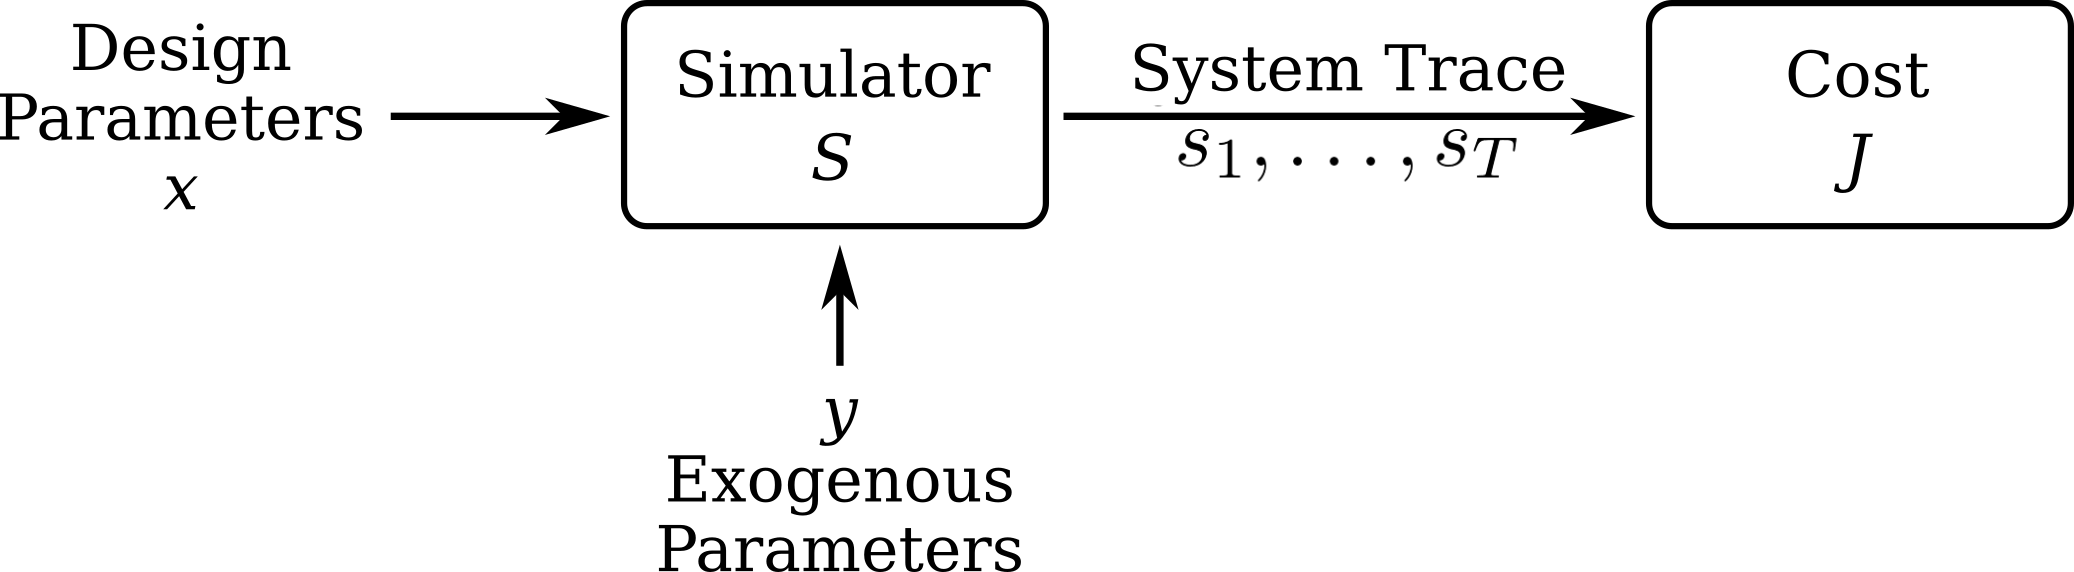
\includegraphics[width=0.6\linewidth]{images/ch5/block_diagram.png}
    \caption{A high-level model of the design and verification problem for an autonomous system. Design optimization involves finding a set of design parameters so that the simulated cost is minimized, while verification involves understanding how changes in the exogenous parameters affect the simulated cost.}
    \label{ch5:fig:block_diagram}
\end{figure}

In this context, we can formalize the design, verification, and verification-guided design tasks as optimization problems. For the time being, we take a worst-case approach to verification, but we will revisit this in Section~\ref{section:global_methods}.

\begin{align}
    \textit{Design: }                     & x = \argmin_{x \in \cX} \expectation_{y \sim \cY}\left[ J(S(x, y)) \right] \label{ch5:eq:design}     \\
    \textit{Verification: }               & y = \argmin_{y \in \cY} J(S(x, y))    \label{ch5:eq:verification}                                    \\
    \textit{Verification-guided design: } & x = \argmin_{x \in \cX} \max_{y \in \cY} J(S(x, y)) \label{ch5:eq:verification_guided_design_minmax}
\end{align}

These problems have been studied in various forms throughout the prior literature, but previous works tend to either use sample-inneficient black-box optimization techniques~\cite{corsoAdaptiveStressTesting2019,corsoSurveyAlgorithmsBlackBox2021a,dingLearningCollideAdaptive2020a,wangAdvSimGeneratingSafetyCritical2021a} or focus on developing application-specific algorithms for certain cases where gradients can be derived~\cite{Schulz_robogami,du2016computational,du2021underwater,ma2021diffaqua,xu_uav_controllers}. The first contribution in this chapter is to expand on these application-specific works to demonstrate how automatic differentiation enables us to easily apply gradient-based optimization methods to solve the design and verification problems.

Unfortunately, while simply feeding AD-derived gradients into off-the-shelf optimizers is a natural (and often effective) first step, it provides few assurances of that our optimized designs will be robust, and does little to connect the results of verification back into the design process. The second contribution in this chapter is to close this gap by developing a framework that uses AD-derived gradients to accelerate adversarial testing.

This chapter presents work published in RSS 2022~\cite{dawsonCertifiableRobotDesign2022a} and IROS 2022~\cite{dawsonRobustCounterexampleguidedOptimization2022}. In the interest of brevity, we defer implementation details to the appendix and focus here on the key ideas, results, and limitations.

\subsection{Efficient design optimization using differentiable simulation}

A natural first instinct when presented with gradients from an automatic differentiation system is to apply a gradient-based optimizer to find low-cost design parameters. This approach is simple (relying on pre-existing optimization methods), flexible (using general-purpose AD libraries to model subsystems with varying levels of abstraction), and efficient (making use of gradients to accelerate the search for high-performing designs).

Although it is possible to directly optimize the objective in~\eqref{ch5:eq:design} to find low-cost design parameters, in many practical use-cases we are interested in designs that are not only low-cost but robust to variation in $y$, which we can encode by regularizing the objective with respect to the variance of the cost:
%
\begin{subequations}\label{ch5:eq:design_optimization_nlp_generic}
    \begin{align}
        \min_{x \in \cX} & \quad \expectation_{y \sim \cY} \Big[ J\circ S\pn{x, y} \Big] + \lambda \rm{Var}_{y\sim\cY}\Big[ J\circ S\pn{x, y} \Big] \label{ch5:eq:design_optimization_objective_generic}
    \end{align}
\end{subequations}
%
To yield a tractable problem, we replace the expectation and variance with unbiased estimates over $N$ samples $y_i \sim \cY, i=1,\ldots,N$.
%
\begin{subequations}\label{ch5:eq:design_optimization_nlp}
    \begin{align}
        \min_{x \in \cX} & \quad \frac{1}{N}\sum_{i=1}^{N} \Big[J\circ S\pn{x, y_i}\Big] + \lambda \left[ \frac{\sum_{i=1}^N \pn{J\circ S\pn{x, y_i}}^2}{N-1} - \frac{\pn{\sum_{i=1}^N J\circ S\pn{x, y_i}}^2}{(N-1)N} \right] \label{ch5:eq:design_optimization_objective}
    \end{align}
\end{subequations}

Since computing this objective requires multiple calls to the simulator $S$, approximating the gradients of~\eqref{ch5:eq:design_optimization_objective} using finite-differences or stochastic multi-sample estimators would incur a large computational cost (requiring $O(N\dim{x})$ calls to $S$). Fortunately, backwards-mode AD allows us to obtain these gradients much more cheaply, with a constant $O(N)$ simulator calls, regardless of the dimension of the search space. On high-dimensional problems, like optimizing a neural network planning system for the multi-robot collaborative manipulation system shown in Fig.~\ref{ch5:fig:mam_hw}, the improved scaling of AD is clearly apparent. In this example, where the cost measures how close the robots were able to maneuver the box to its desired pose (which varies randomly along with uncertain coefficients of friction in the environment), $\dim{x} = 454$ and $N = 512$, so AD requires two orders of magnitude fewer simulator evaluations than a finite-difference scheme.

This improved scaling can be seen empirically if we compare the time required to run L-BFSG-B (a quasi-Newton first-order optimizer) until convergence using both AD-derived and finite-difference gradients. Fig.~\ref{ch5:fig:ablation} shows that although both methods achieve a similar optimal cost, AD-based optimization runs 20x faster (even after accounting for the additional computational overhead of backwards-mode AD).

\begin{figure}[tb]
    \centering
    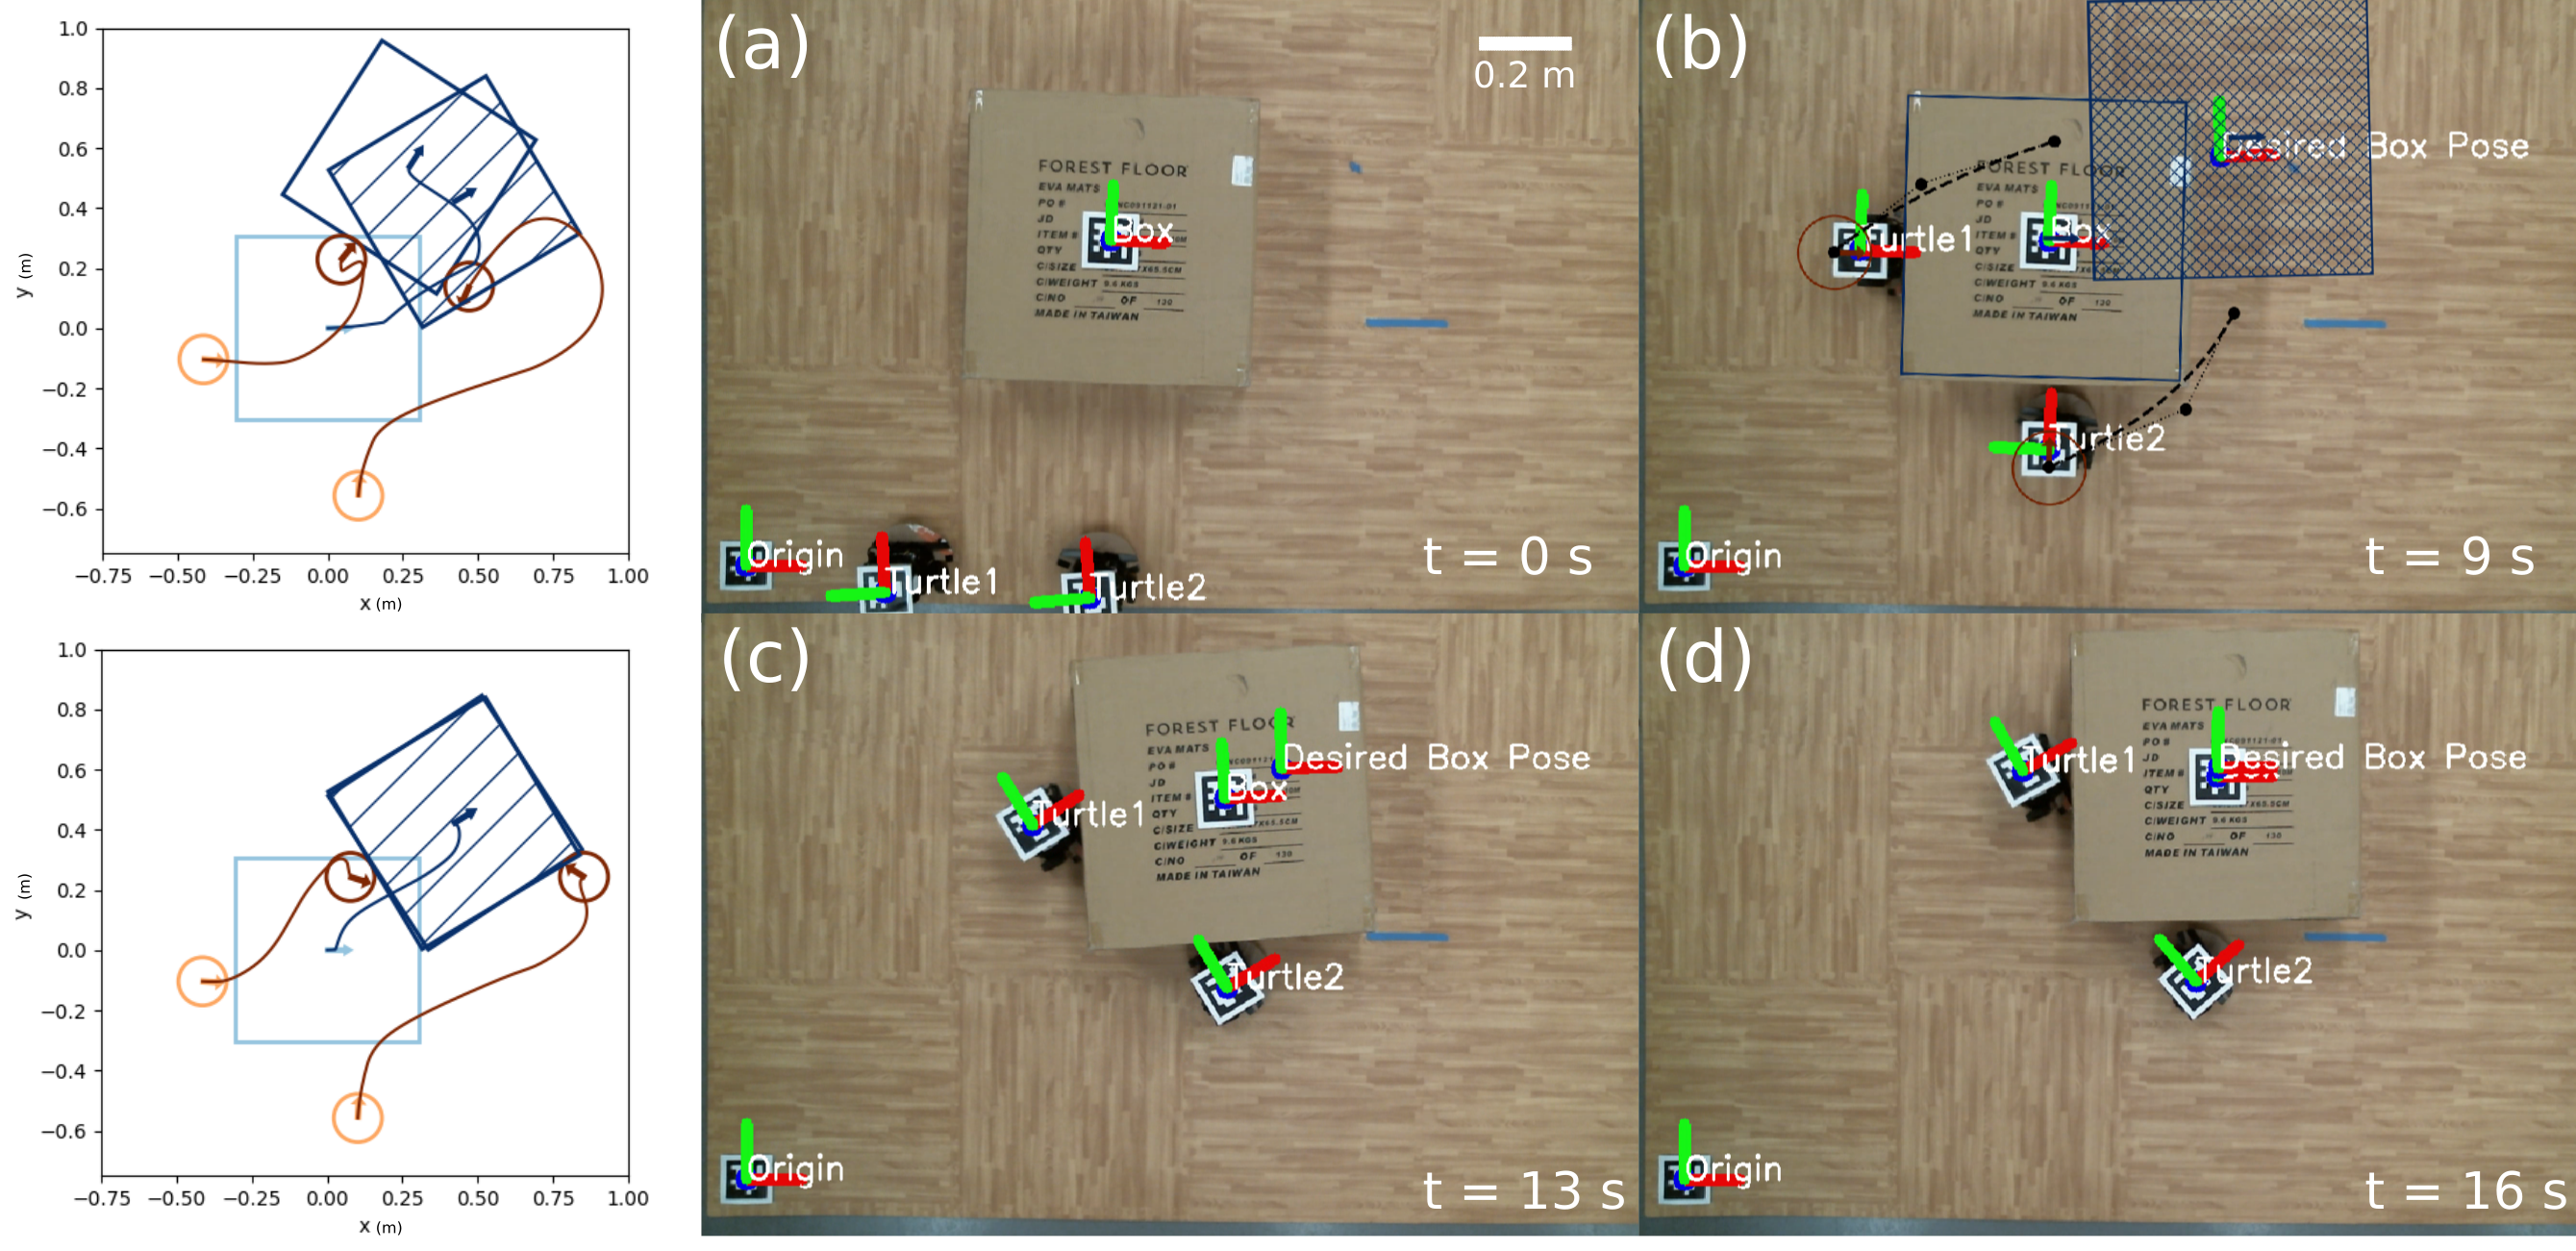
\includegraphics[width=\linewidth]{images/ch5/mam_composite_w_sim.png}
    \caption{Left: Initial (top) and optimized (bottom) manipulation strategies in simulation (light/dark colors indicate initial/final positions, stripes indicate desired position). Right: Optimized manipulation strategy deployed in hardware (video included in the supplementary materials). (a) The robots first move to positions around the box. (b) Using the optimized neural network, the robots plan a cubic spline trajectory pushing the box to its desired location. (c-d) The robots execute the plan by tracking that trajectory.}
    \label{ch5:fig:mam_hw}
\end{figure}

\begin{figure}[t]
    \centering
    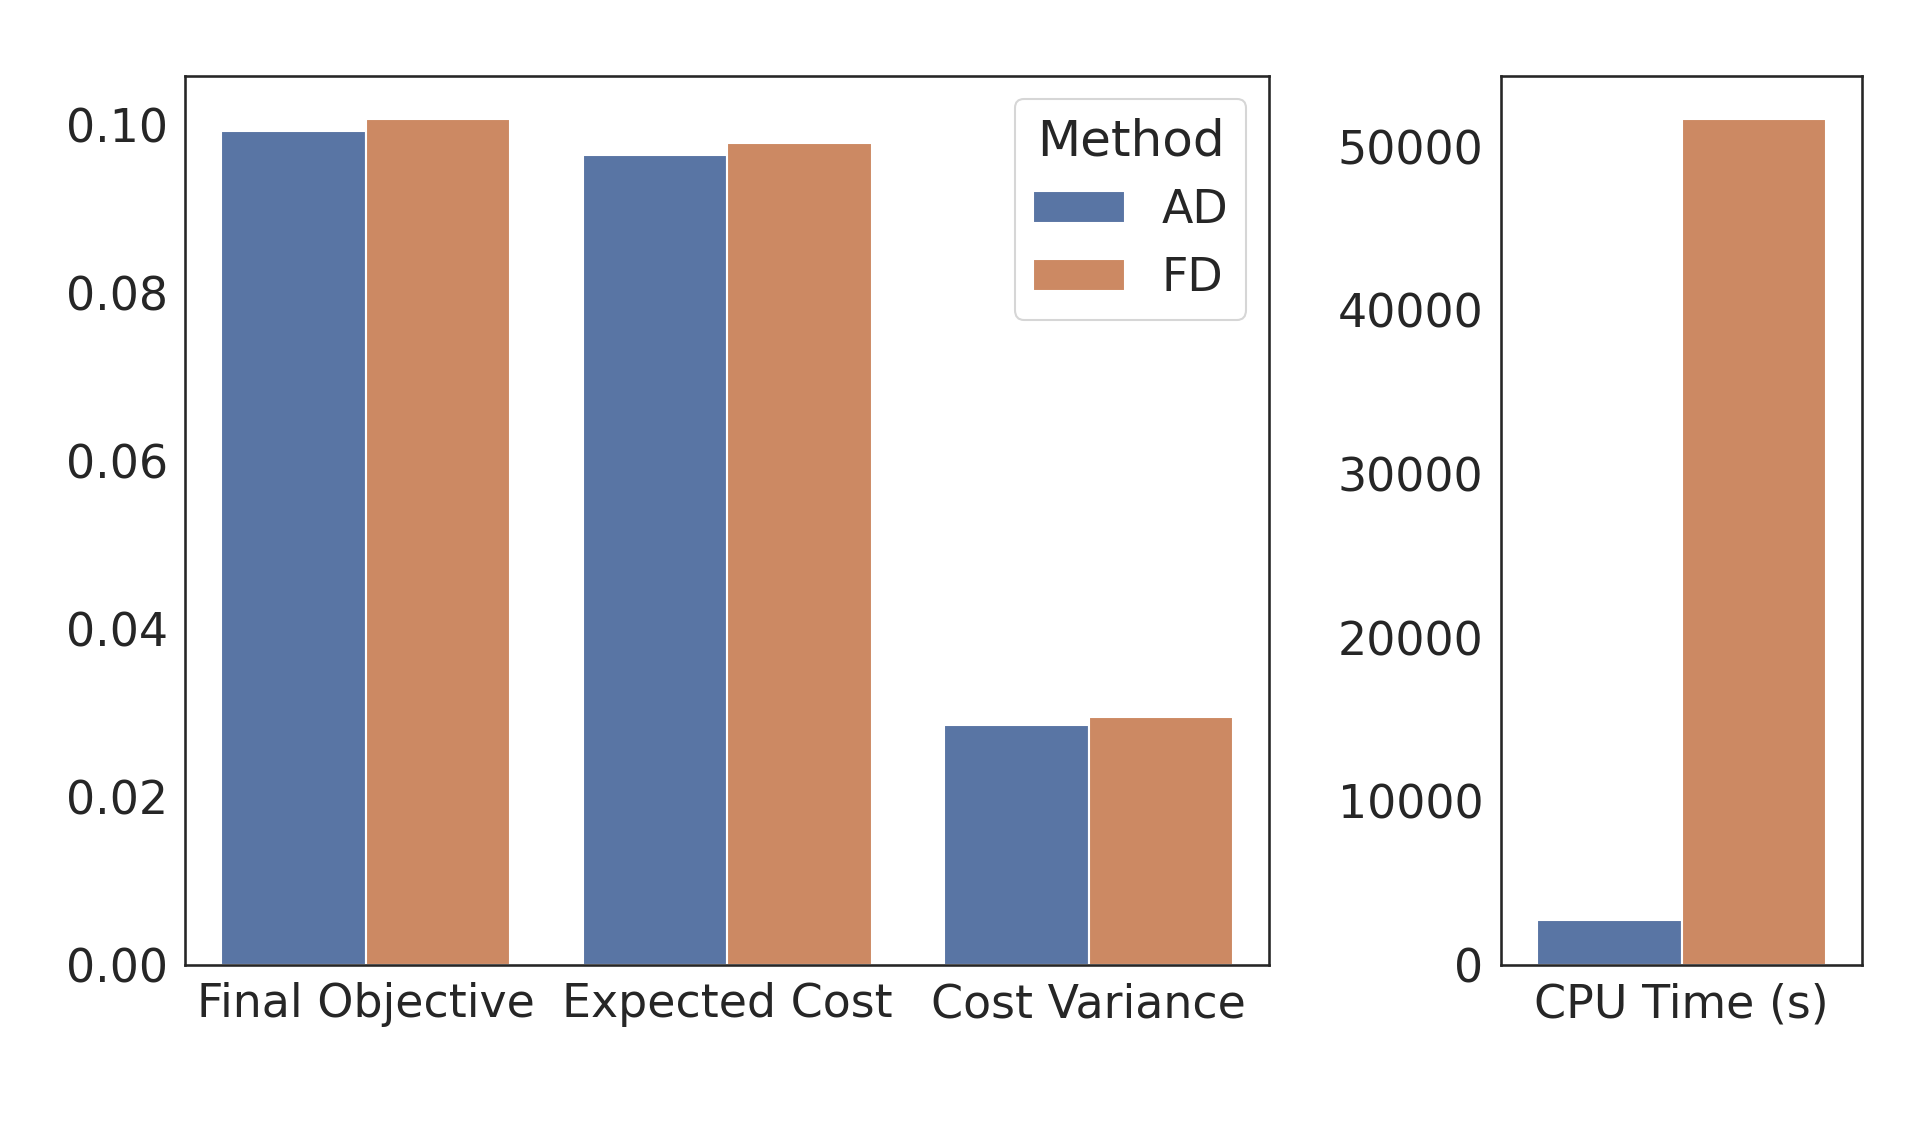
\includegraphics[width=0.7\linewidth]{images/ch5/mam_ablation_ad_fd.png}
    \caption{Improvement of automatic differentiation (AD) over finite differences (FD) on the multi-agent manipulation case study shown in Fig.~\ref{ch5:fig:mam_hw}.}
    \label{ch5:fig:ablation}
\end{figure}

\subsection{Local adversarial testing for verification-guided design}

The results in the previous section show how we can use AD for efficient and robust gradient-based optimization; however, the computational expense of averaging over exogenous parameters makes it difficult to scale to larger systems that may be more difficult to simulate. In addition, in many safety-critical contexts we are interested in verifying not only the average-case but the worst-case behavior.

These difficulties motivate the next contribution of this chapter, where we introduce an adversarial optimization approach to solving the min/max problem~\eqref{ch5:eq:verification_guided_design_minmax}. Of course, solving~\eqref{ch5:eq:verification_guided_design_minmax} to global optimality in the general nonlinear case is intractable. Instead, we take advantage of this game structure to design an iterative algorithm to find the \textit{generalized Nash equilibrium}: the design parameters $x$ and corresponding $y$ such that neither the planner nor the adversary have an incentive to change their choice~\cite{facchineiGeneralizedNashEquilibrium2007a}.

To solve for such an equilibrium, a common strategy is the family of nonlinear Gauss-Seidel-type methods. These methods solve max-min problems like~\eqref{ch5:eq:verification_guided_design_minmax} by alternating between $x$ and $y$, tuning one set of parameters while keeping the others constant; i.e. alternating between the two optimization problems:
\begin{subequations}
    \begin{align}\label{ch5:eq:gauss_seidel}
        x^* & = \argmin_x J(x, y^*) \\
        y^* & = \argmax_y J(x^*, y)
    \end{align}
\end{subequations}
Although these methods are not guaranteed to converge, it is known that if they do, then the convergence point $(x^*, y^*)$ is a Nash equilibrium~\cite{facchineiGeneralizedNashEquilibrium2007a}.

A risk of applying such a simple alternating scheme is that the nonlinear optimization for both $x$ and $y$ can easily get caught in local minima, which increases the risk of ``overfitting'' the design to a particular value of $y^*$. To mitigate the risk of overfitting and improve the robustness of our optimized design, we extend the standard Gauss-Seidel method with two ideas from the machine learning and optimization literature. First, we take inspiration from the success of domain randomization in robust machine learning~\cite{tobinDomainRandomizationTransferring2017}: instead of optimizing $x$ with respect to a single fixed $y^*$, we can maintain a dataset $\cY_N = \set{y_i}_{i=1,\ldots,N}$ and optimize the performance of $x$ across all of these samples:
\begin{subequations}
    \begin{align}\label{ch5:eq:gauss_seidel_domain_randomization}
        x^* & = \argmin_x \mathbb{E}_{\cY_N} \left[ J(x, y_i) \right] \\
        y^* & = \argmax_y J(x^*, y)
    \end{align}
\end{subequations}

This domain-randomized objective is similar to that used in the previous section and has the potential to improve the robustness of the resulting equilibria, but it is relatively sample inefficient; it may require a large number of random samples $y_i$ to cover the range of possible system behaviors. To address this sample inefficiency, we take inspiration from a second idea in the optimization and learning literature: learning from counterexamples~\cite{changNeuralLyapunovControl2019}. The key insight here is that we can do better than simply randomly sampling $y_i$; we can use the values of $y^*$ found during successive iterations of the Gauss-Seidel process as high-quality counterexamples to guide the optimization of $x$. This insight results in our counterexample-guided Gauss-Seidel optimization method, which is outlined in pseudocode in Algorithm~\ref{ch5:alg:cg_gs}.

Our algorithm proceeds as follows. We begin by initializing the dataset with $N_0$ i.i.d. examples $y_i$, then we alternate between solving the two optimization problems in~\eqref{ch5:eq:gauss_seidel_domain_randomization}. At each iteration, we add our current estimate of the adversary's best response $y^*$ to the dataset, and we stop either when the algorithm reaches a fixed point (the adversary's best response after solving~\eqref{ch5:eq:gauss_seidel_domain_randomization} is the same as the best response from the previous round) or when a maximum number of iterations is reached. As we will show in our experiments in the next section, this counterexample-guided optimization achieves a higher sample efficiency than simple domain randomization ---  it finds designs that are more robust to adversarial disturbance while considering a much smaller dataset. Although our use of nonlinear optimization means that our algorithm is not complete, we find empirically that it succeeds in finding a satisfactory design in the large majority of cases.

It is important to note that this algorithm is enabled by automatic differentiation; without access to the gradients of $J$ it would be much more difficult to solve the subproblems in lines~\ref{ch5:alg:opt_theta} and~\ref{ch5:alg:opt_chi} of Algorithm~\ref{ch5:alg:cg_gs}. We are not aware of any approaches that make use of automatically-derived gradients with respect to disturbance parameters for adversarial verification-guided optimization.

\begin{algorithm}
    \caption{Counterexample-guided Gauss-Seidel method for solving robust planning problems}\label{ch5:alg:cg_gs}
    \DontPrintSemicolon
    \KwInput{Starting dataset size $N_0$\\\phantom{Input: } Maximum number of iterations $M$}
    \KwOutput{Optimized design parameters $x^*$\\\phantom{Output: } Dataset of counterexamples $\set{y^*}$}
    $\set{y^*} \gets $ $N_0$ examples $y_i \in \cY$ sampled uniformly i.i.d.\;
    $y^*_{prev} \gets \varnothing$\;
    \For{$i \in \set{1, \ldots, M}$}
    {
        $x^* = \argmin_x \mathbb{E}_{\cY_N} \left[ J(x, y_i) \right] \label{ch5:alg:opt_theta}$ \;
        $y^* = \argmax_y J(x^*, y)$ \label{ch5:alg:opt_chi} \;
        \If{$y^* = y^*_{prev}$}{\Break}
        $y^*_{prev} \gets y^*$\;
        Append $y^*$ to $\set{y^*}$\;
    }
    \KwRet{$x^*$, $\set{y^*}$}
\end{algorithm}

To validate this approach, we can use two case studies involving planning and control for the satellite rendezvous problem posed in~\cite{jewisonSpacecraftBenchmarkProblem2016}. We define this planning problem using signal temporal logic (STL), which provide a formal language for capturing complex behavioral requirements and specifying how a robot behaves over time. For a brief introduction to the syntax and semantics of STL, see~\cite{dawsonRobustCounterexampleguidedOptimization2022}. By restricting this case study to focus on planning, we are able to benchmark against state-of-the-art planning algorithms to show the robustness and scalability benefits of our adversarial optimization-based approach. We implement a smooth differentiable version of STL following the approach in~\cite{leungBackPropagationSignalTemporal2021,pantSmoothOperatorControl2017}.

In this satellite rendezvous problem, the goal is to maneuver a chaser satellite to catch a target satellite. In this setting, we construct STL specifications for two rendezvous missions: a simple low-speed rendezvous and a more complex loiter-then-rendezvous mission, illustrated in Fig.~\ref{ch5:fig:mission_specs}. The STL specifications for each mission, $\psi_1$ and $\psi_2$, are given formally as:
\begin{align*}
    \psi_1                   & = \psi_\text{reach target} \wedge \psi_\text{speed limit}                           \\
    \psi_2                   & = \psi_\text{reach target} \wedge \psi_\text{speed limit} \wedge \psi_\text{loiter} \\
    \psi_\text{reach target} & = \eventually \pn{r \leq 0.1}                                                       \\
    \psi_\text{speed limit}  & = \pn{r \geq 2.0} \until\ \always \pn{v \leq 0.1}                                   \\
    \psi_\text{loiter}       & = \eventually \always_{[0, T_{obs}]} \pn{2.0 \leq r \wedge r \leq 3.0}
\end{align*}
where $r = \sqrt{p_x^2 + p_y^2 + p_z^2}$ and $v = \sqrt{v_x^2 + v_y^2 + v_z^2}$.

These formulae can be read as follows: $\psi_\text{reach target}$ specifies that ``the chaser eventually comes within \SI{0.1}{m} of the target'', $\psi_\text{speed limit}$ specifies that ``once the chaser is within \SI{2.0}{m} of the target, its speed cannot exceed \SI{0.1}{m/s}'', and $\psi_\text{loiter}$ specifies that ``at some point during the mission, the chaser should spend $T_{obs}$ seconds between 2--\SI{3}{m} away from the target''. The two missions are build from these three building blocks: mission 1 includes the ``reach target'' and ``speed limit'' requirement, while mission 2 includes all three requirements.

For each mission, the design parameters $x$ include both state/input waypoints along a planned trajectory and the feedback gains used to track that trajectory, and the exogenous parameters $y$ represent bounded uncertainty in the initial state of the chaser ($p_x(0), p_y(0) \in [10, 13]$, $p_z(0) \in [-3, 3]$, $v_x(0), v_y(0), v_z(0) \in [-1, 1]$). We use a \SI{200}{s}-long simulation with a \SI{2}{s} timestep for both missions, and $T_{obs} = \SI{10}{s}$.

\begin{figure}[t]
    \centering
    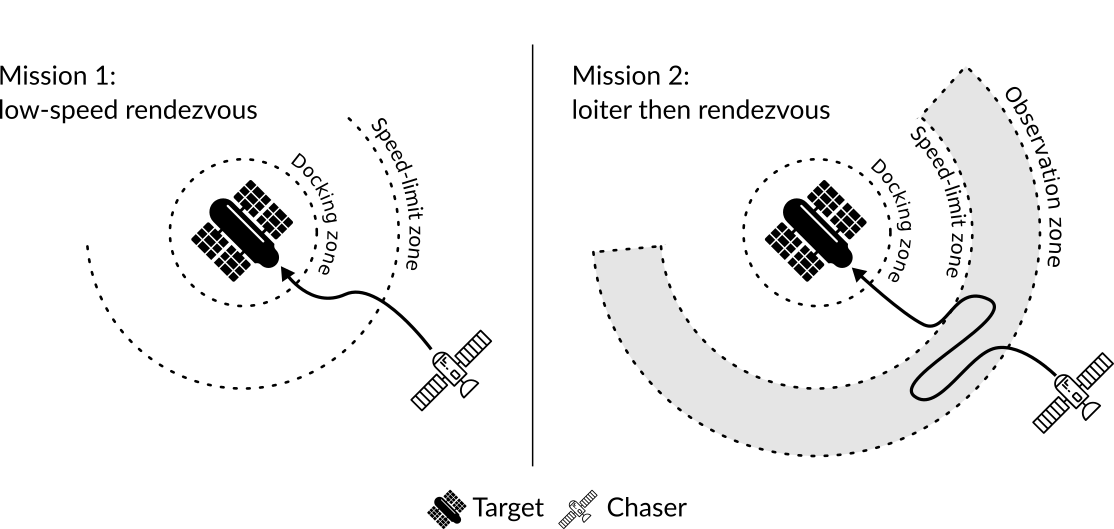
\includegraphics[width=0.7\linewidth]{images/ch5/satellite_missions.png}
    \caption{Two satellite rendezvous missions used to test our adversarial optimization framework. In the first mission, the chaser satellite must eventually reach the target while respecting a maximum speed constraint in the region immediately around the target. In the second mission, the chaser must still reach the target and obey the speed limit, but it must also loiter in an observation region for some minimum time before approaching. The first mission requires an STL formula with three predicates and three temporal operators, while the second mission requires five predicates and five temporal operators.}
    \label{ch5:fig:mission_specs}
\end{figure}

For each mission $i=1, 2$, we define a cost function as $J_i = -\rho_i + \lambda I$, where $\rho_i = \rho(\psi_i, S(x, y), 0)$ is the STL robustness margin at the start of the trajectory (i.e. how satisfied/unsatisfied the requirements are), $I$ is the total impulse required to execute the maneuver (in Newton-seconds), and $\lambda = 5\times10^{-5}$. By applying our iterative counterexample-guided optimization strategy to this problem, we find the optimized trajectories for mission 1 and 2 shown in Fig.~\ref{ch5:fig:mission_trajs} along with the worst-case $y$. In these examples, we use $N_0=8$ initial examples and $M=10$ maximum rounds, but the algorithm converges in less than 10 rounds in all trials. In both missions, our approach reliably finds a solution that remains feasible despite worst-case variation in the exogenous parameters, achieving a positive STL robustness margin in $>90\%$ of trials in each case. Our counterexample-guided approach requires an average of \SI{53.7}{s} to solve mission 1 and \SI{194.2}{s} to solve mission 2 (averaged across 50 trials).

\begin{figure}[t]
    \centering
    \begin{subfigure}[t]{0.4\linewidth}
        \centering
        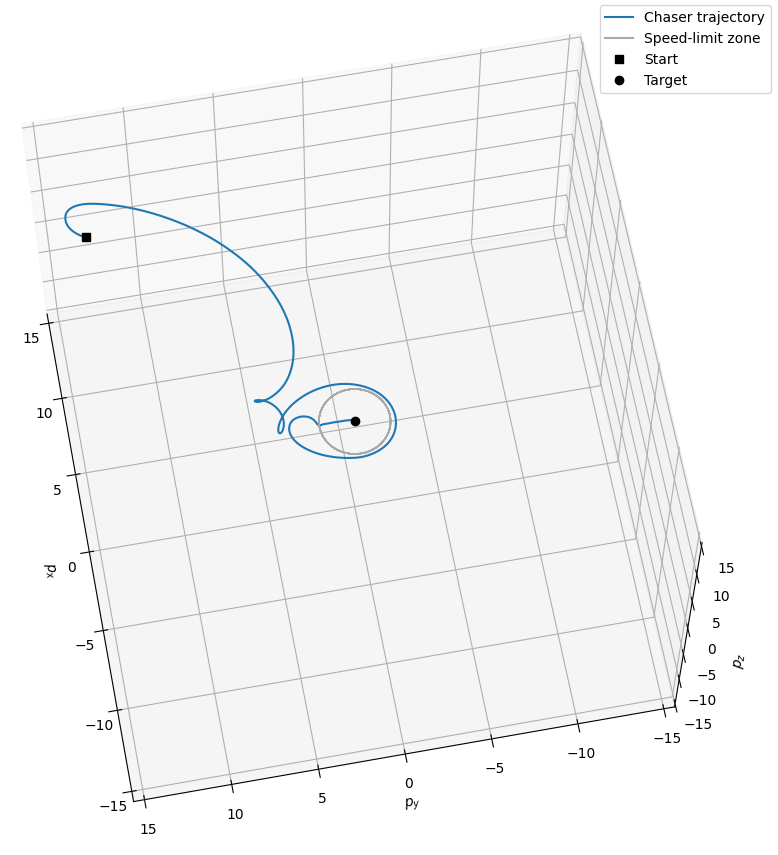
\includegraphics[width=\linewidth]{images/ch5/satellite_mission1_traj.png}
        \caption{Mission 1}
    \end{subfigure}
    \begin{subfigure}[t]{0.4\linewidth}
        \centering
        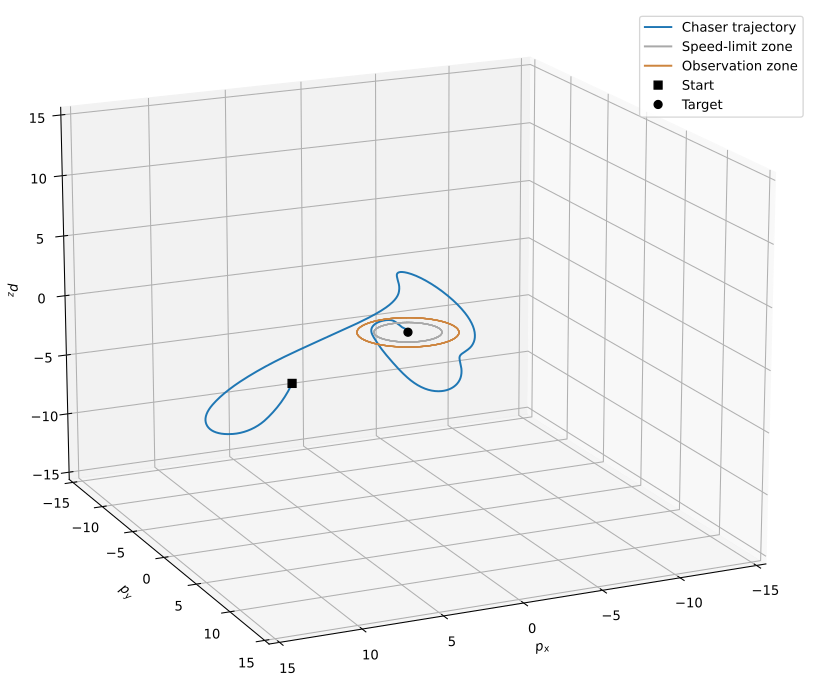
\includegraphics[width=\linewidth]{images/ch5/satellite_mission2_traj.png}
        \caption{Mission 2}
    \end{subfigure}%
    \caption{(a) The optimized trajectory found using our counterexample-guided optimization strategy for mission 1 (rendezvous with speed constraint). The chaser satellite only enters the speed-limit zone once it has slowed down sufficiently. (b) The optimized trajectory for mission 2 (loiter then rendezvous with speed constraint), satisfying the additional mission requirement of spending time in the observation region before approaching the target.}
    \label{ch5:fig:mission_trajs}
\end{figure}

To quantify the advantage of our AD-enabled adversarial optimization method relative to the state-of-the-art, there are two salient comparisons. First, what advantage does adversarial optimization have relative to domain randomization? Second, since we are solving a specialized motion planning problem, how does our method compare against application-specific solvers for this STL planning problem?

To answer the first question, we compare our adversarial method with non-adversarial optimization with domain randomization with 64 and 32 samples, as well as non-adversarial optimization without any domain randomization (1 sample). To answer the second question, we compare with a mixed-integer programming (MIP) approach to solving STL planning problems~\cite{sunMultiagentMotionPlanning2022}. The results of this comparison are shown in~\ref{ch5:fig:stl_comparisons}. All experiments were run on a laptop computer with \SI{8}{GB} RAM and a \SI{1.8}{GHz} 8-core processor, with no GPU, and results are averaged over 50 random seeds.

We find that our method is consistently more robust than prior methods; in the first mission, it satisfies the STL specification in all but 3 trials, despite adversarial disturbances. For comparison, the next-best method (domain randomization with 64 samples) failed to solve the first mission in 14 out of 50 trials and took more than twice as long on average to find a plan (\SI{114.3}{s} as opposed to \SI{53.7}{s} for our method). This advantage is due to the quality of the examples used during optimization; instead of 64 random samples, our method uses 8 initial random samples and between 1 and 4 counterexamples (median 2) representing worst-case variation in $y$, making our method much more sample-efficient. This pattern also holds on the second mission, where 64-sample domain randomization takes more than twice as long as our method and fails to satisfy the STL specification in 17 out of 50 trials (compared to only 4 failures for our method). Our method required a median of 2 counterexamples in addition to the 8 initial examples to solve the second mission (the slowest trial required 7 additional examples).

We also find that our method finds more robust solutions than the MIP method, since MIP cannot tractably consider variation in $y$ (the MIP method is also unable to find a feasible solution within \SI{500}{s} in 16 out of 50 trials). MIP's performance also suffers due to discretization error, since we were forced to discretize the continuous-time dynamics with relatively few knot points (one every \SI{2}{s}) to yield a tractable MIP optimization problem.


\begin{figure}[t]
    \centering
    \begin{subfigure}[t]{0.45\linewidth}
        \centering
        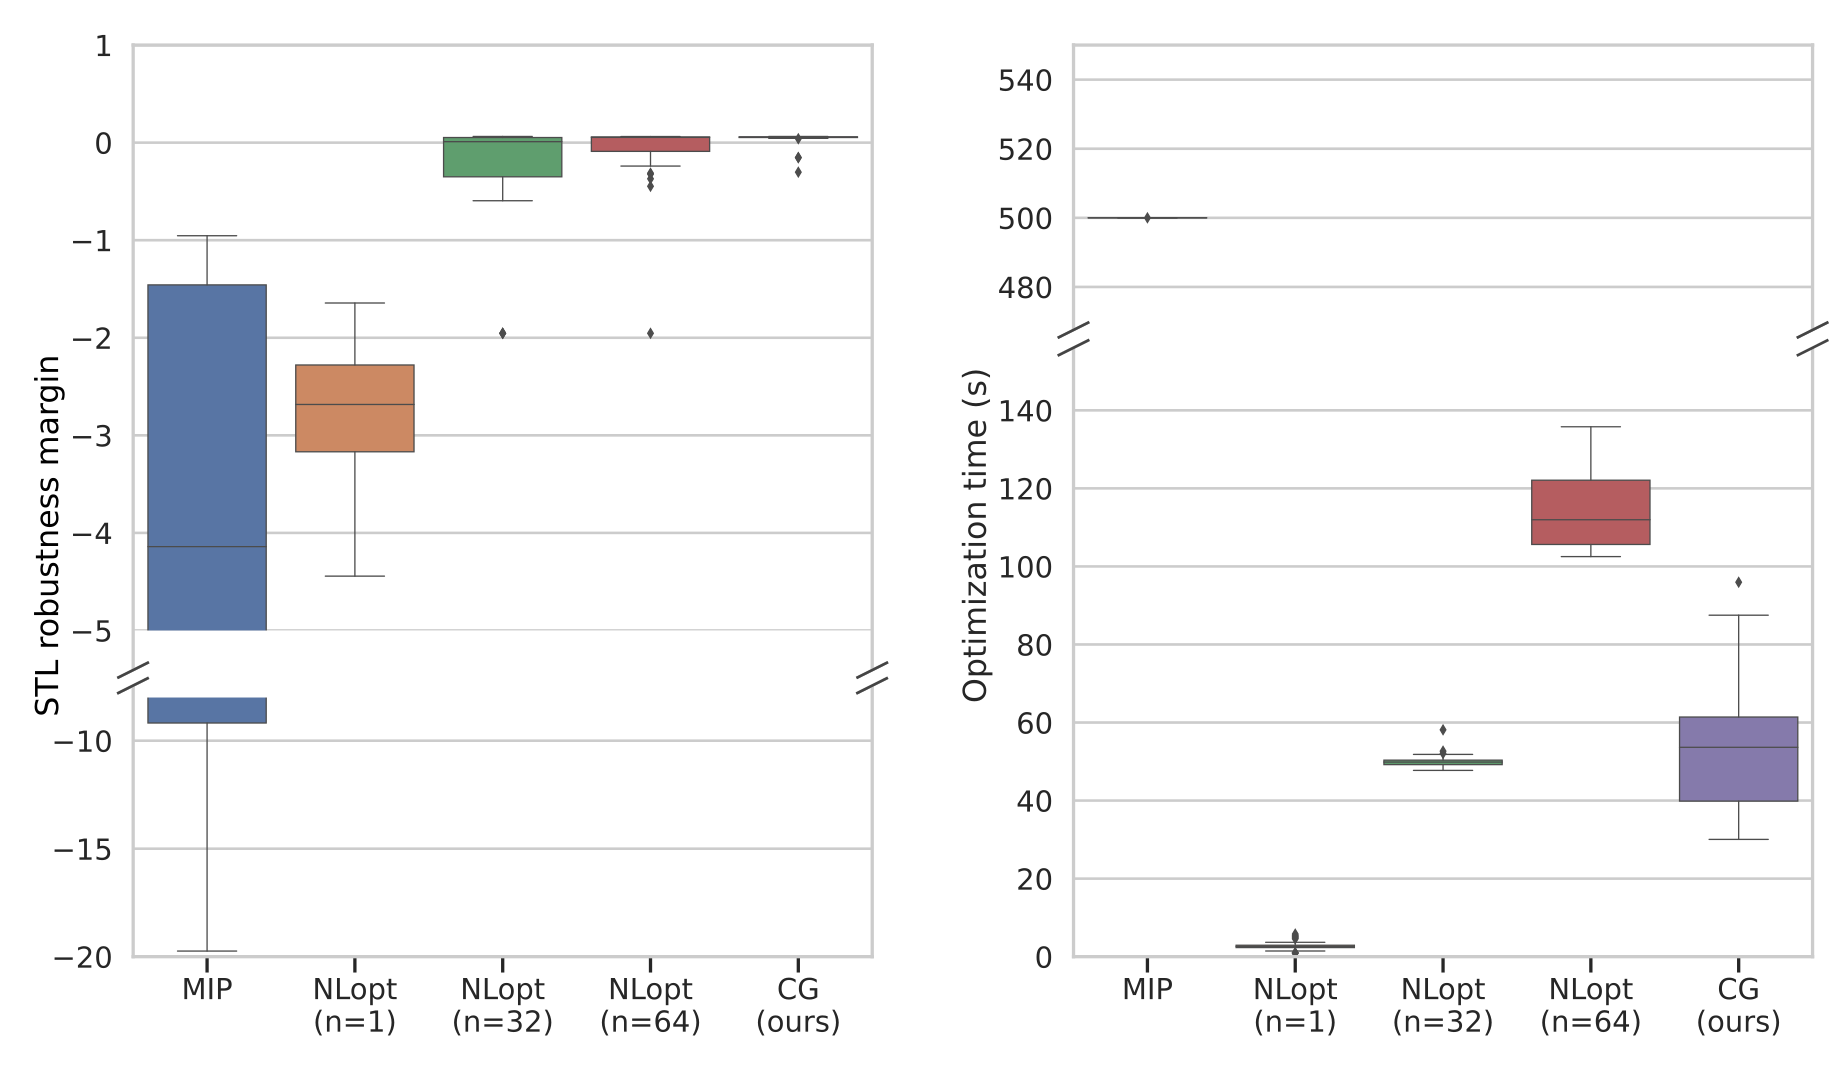
\includegraphics[width=\linewidth]{images/ch5/mission_1_comparison.png}
        \caption{Mission 1}
    \end{subfigure}
    \begin{subfigure}[t]{0.45\linewidth}
        \centering
        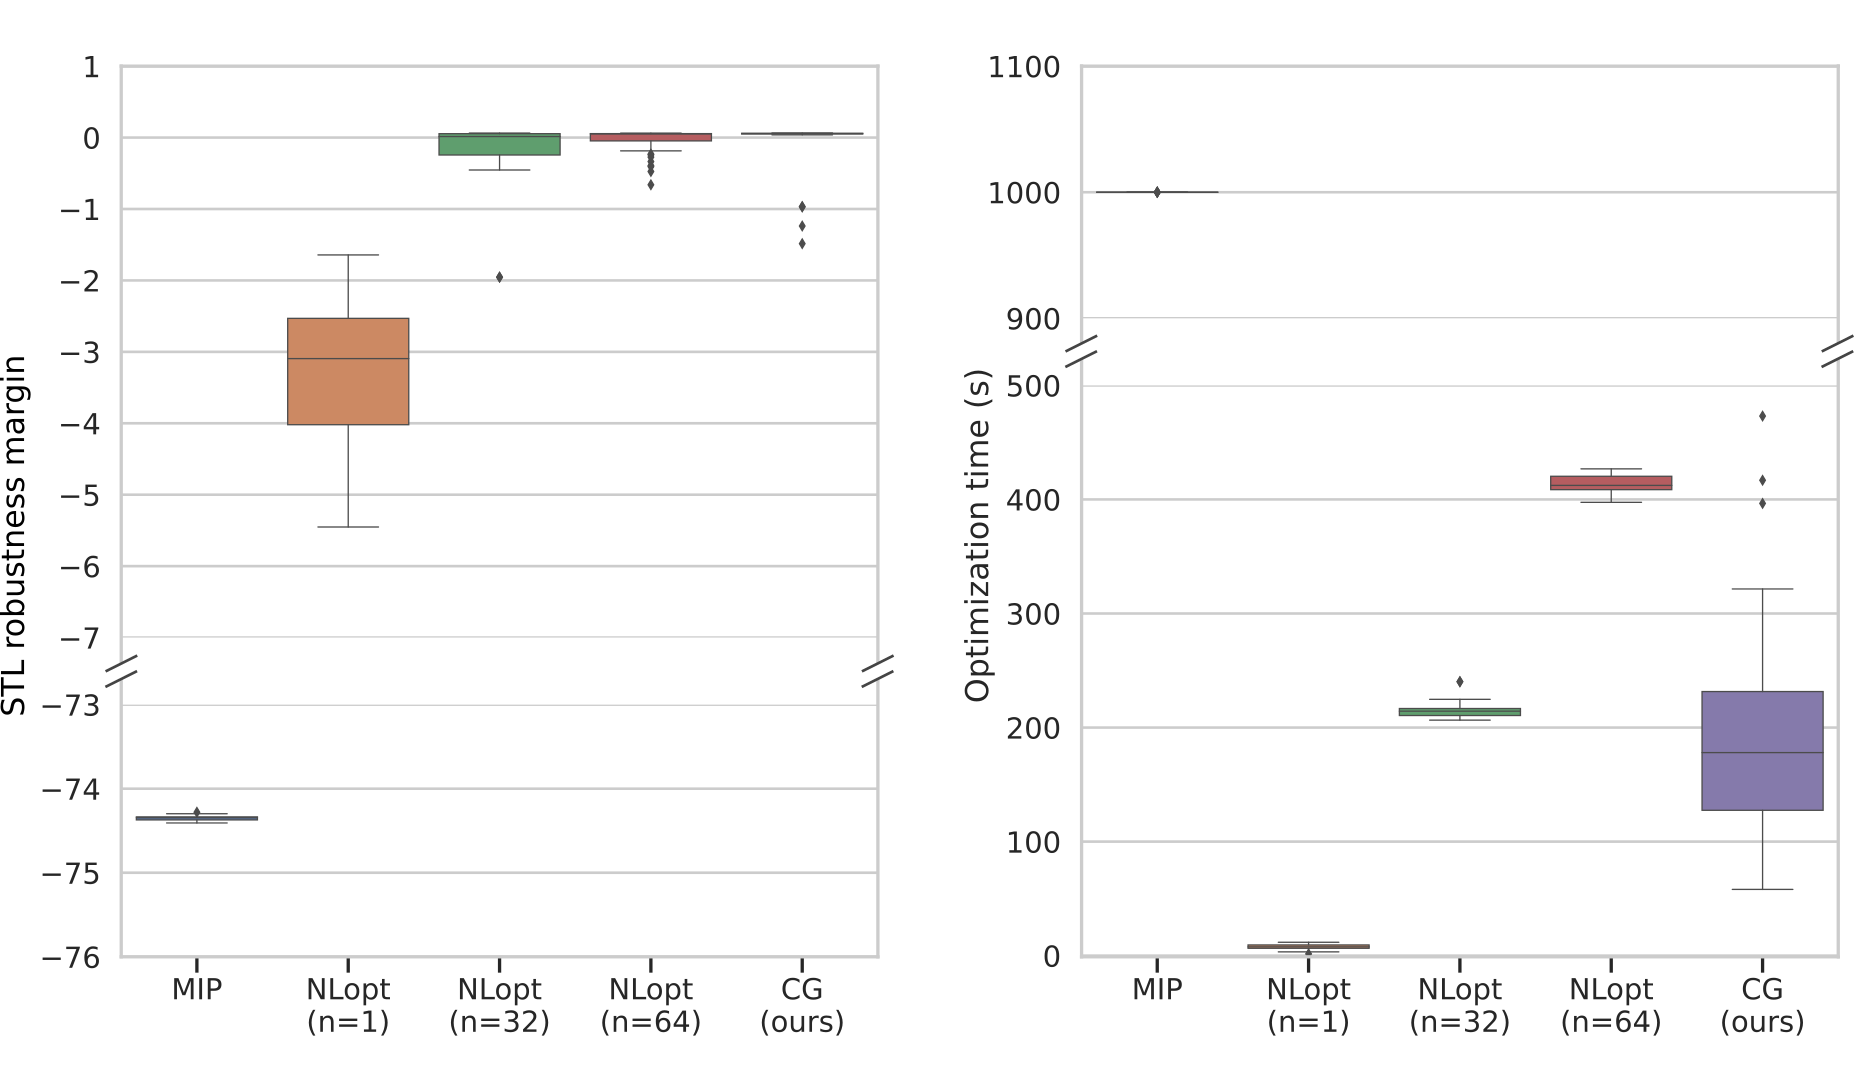
\includegraphics[width=\linewidth]{images/ch5/mission_2_comparison.png}
        \caption{Mission 2}
    \end{subfigure}%
    \caption{Comparison of different STL planning methods on mission 1 (a) and 2 (b), averaged over 50 random seeds. (left subfigures) The robustness margin $\rho(\psi_1)$ computed for the optimized design parameters and worst-case exogenous parameters. (right subfigures) The planning time required by each method. Our method (CG) achieves much higher robustness than all other methods (satisfying the STL specification despite adversarial perturbations in all but 3 instances) and runs twice as fast as the next-most-robust method.}
    \label{ch5:fig:stl_comparisons}
\end{figure}

\subsection{Discussion \& Limitations}

In this chapter, I have presented my previous work on auto-diff-enabled design optimization and verification, with three key takeaways. The first two takeaways are technical and regard the utility of AD for design optimization and verification. First: AD enables a flexible, general-purpose framework for optimizing and verifying a wide-range of robotics problems, with support for multiple interacting subsystems, rich dynamics, and complex task specifications. Second: the use of gradients from AD enables solution methods (such as variance regularization and adversarial optimization) that would be much more computationally expensive if these gradients had to be estimated by other means. The final takeaway is agnostic to the use of AD and concerns how using adversarial optimization can improve both the robustness and the sample efficiency of design optimization (relative to domain randomization).

The main limitation of the work presented in this chapter is its reliance on local gradient-based optimization. As a result, there is still a need for algorithms that take a more global perspective, particularly for verification, which we will introduce in the next chapter.

% Advantages of the differentiable simulation perspective

% Connection to how it can impact working engineers

% Limitations of the local perspective, set up the next section

%!TEX root = ./main.tex

\section{Global methods for design and verification}\label{section:global_methods}

In the previous chapter, we introduced local gradient-based optimization methods for design, both using standard optimization and adversarial verification-guided optimization. However, there are three notable drawbacks to these approaches.

\begin{enumerate}
    \item \textbf{Risk of local minima: } Local gradient-based optimizers are greedy and prone to getting stuck in local minima. This risk is particularly important in verification use cases, since converging to a set of exogenous parameters that is far from the true worst-case could lead the system designer to falsely believe that their system is safe.
    \item \textbf{Lack of diversity in adversarial examples: } When verifying a system, it is important to consider a diverse set of failure modes. However, optimization-based approaches have difficulty balancing exploration with exploitation, often simply converging to the nearest local optimum.
    \item \textbf{Sensitivity to gradient quality: } Many robotic systems, particularly those involving contact or vision, have dynamics that are not differentiable everywhere, as we assumed in the previous chapter. Even when these dynamics are smoothed, there are still regions where the gradients can be poorly conditioned (i.e. arbitrarily large) or flat, which will cause a gradient-based optimizer to diverge or get stuck.
\end{enumerate}

In this chapter, we will address all of these drawbacks by re-framing the optimization and verification problems as Bayesian inference problems, which we will then solve using gradient-accelerated Markov Chain Monte Carlo (MCMC) methods. We will demonstrate empirically how this Bayesian inference framework provides improved performance (in both convergence speed and solution quality) over both gradient-based and gradient-free optimization methods. The results in this chapter represent ongoing work that has been submitted to NeurIPS 2023 and CoRL 2023.

% Motivate this section by framing the limitations of local methods in the context of an engineer exploring the design space.

% Introduce the capabilities that we want to provide for an engineer: predicting the different ways in which an autonomous system might fail

% Once we have the failure modes, updating the design to mitigate those failure modes.

% Provide a motivating example - SCOPF (others?)

\subsection{From optimization to inference}

To motivate the switch from optimization to inference, consider the toy example of optimizing the cost landscape shown on the left in Fig.~\ref{ch6:fig:toy_example}. This cost function has local minima at $x = -0.544$ and $x = 0.919$ (the latter represents the true global minimum). If initialized with $x < 0$, a local gradient-based optimizer will naturally converge to the sub-optimal local minimum at $x = -0.544$ (the square in Fig.~\ref{ch6:fig:toy_example}), missing the global minimum (marked by a circle). We can see this behavior in Fig.~\ref{ch6:fig:toy_example_convergence}, which plots the convergence of gradient-based optimization with 5 different random starting positions $x\sim\cN(-1.5, 0.1)$. All 5 runs converge to the suboptimal local minimum at $x = -0.544$.

To avoid getting stuck in this local minimum, we can convert the optimization $\argmin_x U(x)$ into the inference problem of sampling from the unnormalized probability density $x \sim p(x) \propto e^{-U(x)}$. This distribution is shown on the right in Fig.~\ref{ch6:fig:toy_example}. We can see that the distribution is bimodal, with a peak at the suboptimal local minimum and a larger peak at the global minimum. By sampling from this distribution, we can find the global minimum with high probability (this is the so-called \textit{Optimization as Inference} approach~\cite{maSamplingCanBe2019,levineReinforcementLearningControl2018a}). In practice, we can approximately sample from this distribution using Markov Chain Monte Carlo (MCMC) methods, which we will discuss in more detail shortly. The benefit of these methods is that they balance exploring different regions of the distribution with exploiting high-likelihood areas; we can see this behavior in Fig.~\ref{ch6:fig:toy_example_convergence}, which shows the convergence of Metropolis-adjusted Langevin (MALA) MCMC, a gradient-based inference method, on the same cost landscape over 5 different random seeds. MALA is able to converge to the global minimum with high probability, while gradient-based optimization gets stuck in the local minimum.

\begin{figure}[tb]
    \centering
    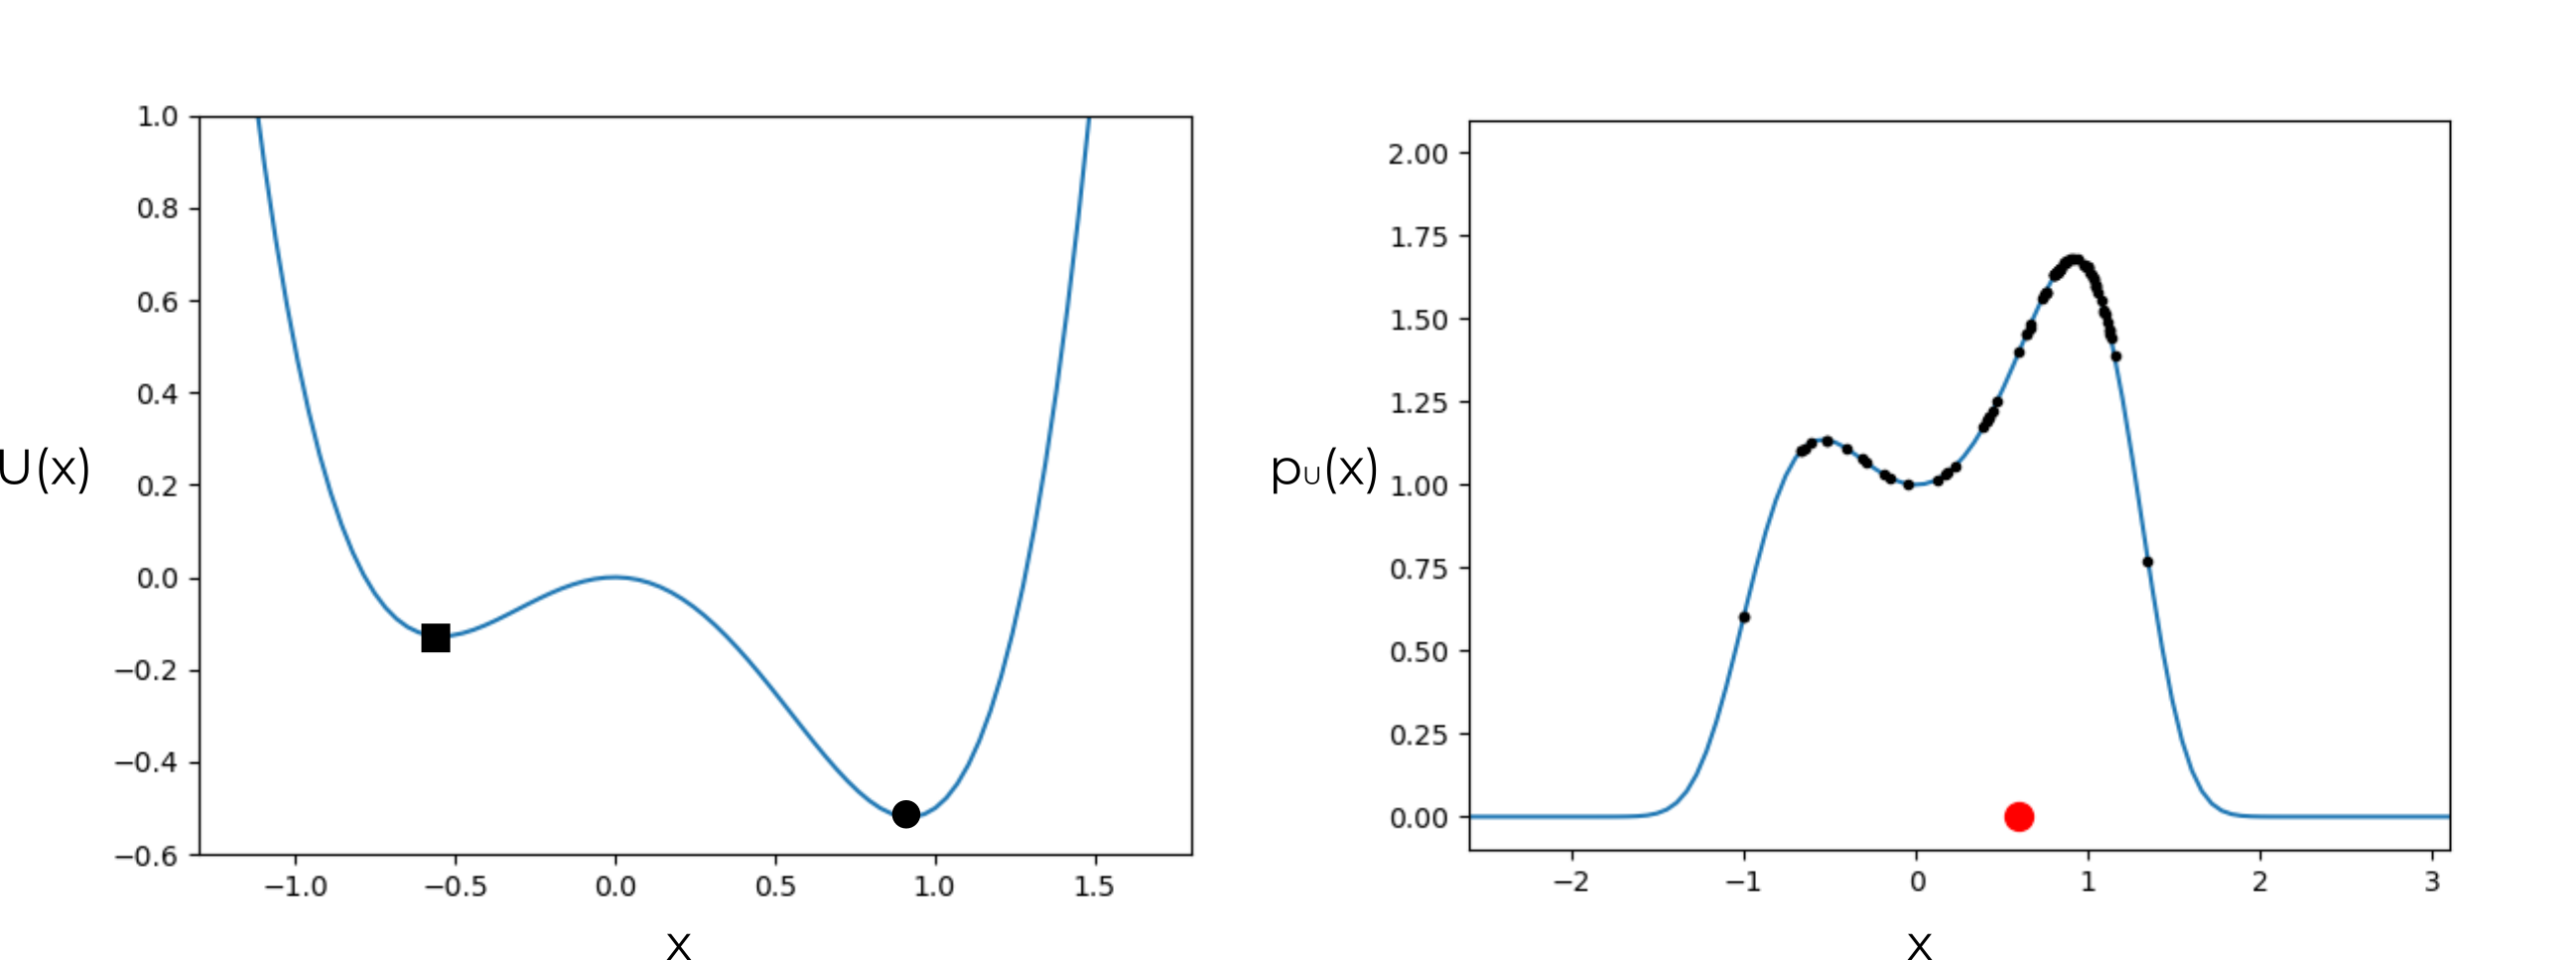
\includegraphics[width=0.6\linewidth]{images/ch6/sampling_as_optimization.png}
    \caption{Left: a simple bimodal cost landscape $U(x) = x^4 - 0.5 x^3 - x^2$, with a locally optimal solution at $x\approx -0.544$ and a global optimum at $x\approx 0.919$. Right: the corresponding unnormalized likelihood $p(x) \propto e^{-U(x)}$, showing samples drawn from this distribution (black dots) and the average of 100 samples (red dot).}
    \label{ch6:fig:toy_example}
\end{figure}

\begin{figure}[tb]
    \centering
    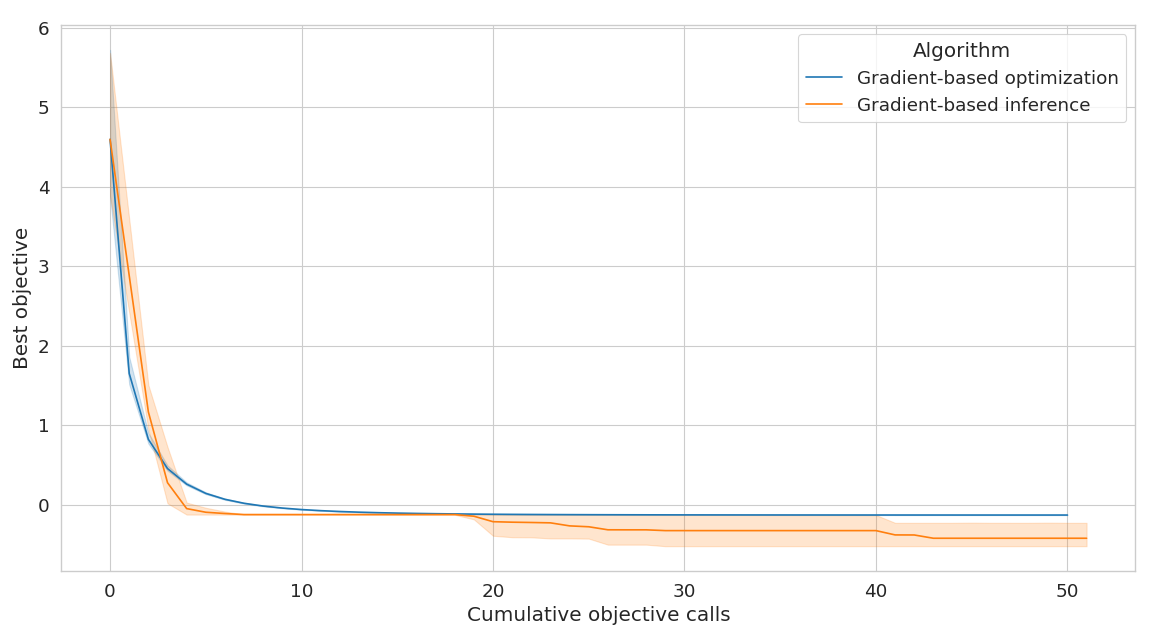
\includegraphics[width=0.6\linewidth]{images/ch6/double_well_gd_mala.png}
    \caption{Convergence of gradient-based optimization and inference (Metropolis-adjusted Langevin) on the double-well cost landscape from Fig.~\ref{ch6:fig:toy_example}, showing how the optimization method gets stuck in a local minimum while the inference method is able to escape and find the global minimum.}
    \label{ch6:fig:toy_example_convergence}
\end{figure}

A wide variety of MCMC algorithms exist to sample from arbitrary non-normalized probability distributions~\cite{geyerIntroductionMarkovChain2011}; common variants include Random-walk Metropolis-Hastings (RMH), Hamiltonian Monte Carlo (HMC), unadjusted Langevin (ULA), and MALA. RMH is gradient-free, while HMC, ULA, and MALA are both gradient-based. MALA, which can be seen as a single-step version of HMC, is outlined in Algorithm~\ref{ch6:alg:mala}. Like all MCMC algorithms, it defines a Markov chain with a transition rule designed to preserve the so-called detailed balance condition, which ensures that the stationary distribution of the Markov chain is the same as the target density (see~\cite{geyerIntroductionMarkovChain2011,aiama} for a more complete introduction). MALA defines a transition rule that begins by proposing a candidate new state in line~\ref{ch6:alg:mala:step} by combining a gradient-driven drift term with a Gaussian diffusion term. The candidate state is accepted with probability $P_{accept}$ in line~\ref{ch6:alg:mala:mh}, which is proportional to the ratio of the target density at the candidate state and the current state. If the candidate state is accepted, it becomes the new current state; otherwise, the current state is repeated. The algorithm is run for $K$ steps, and the final state is returned as the sample from the target density.

\begin{algorithm}
    \caption{Metropolis-adjusted Langevin algorithm (MALA,~\cite{maSamplingCanBe2019,robertsLangevinDiffusionsMetropolisHastings2002})\label{ch6:alg:mala}}
    \DontPrintSemicolon
    \KwInput{Initial $x_0$, steps $K$, stepsize $\tau$, density $p(x)$.}
    \KwOutput{A sample drawn from $p(x)$.}
    \For{$i = 1, \ldots, K$}
    {
    Sample $\eta \sim \cN(0, 2\tau I)$ \Comment{Gaussian noise}\;
    $x_{i+1} \gets x_i + \tau \nabla \log p(x_i) + \eta$ \Comment{Propose next state}\;\label{ch6:alg:mala:step}
    $P_{accept} \gets \frac{p(x_{i+1}) e^{-||x_i - x_{i+1} - \tau \nabla \log p(x_{i+1})||^2 / (4\tau)}}{p(x_{i}) e^{-||x_{i+1} - x_{i} - \tau \nabla \log p(x_{i})||^2 / (4\tau)}}$ \;
    With probability $1 - \min(1, P_{accept})$:
    \hspace{2em}$x_{i+1} \gets x_{i}$ \Comment{Accept/reject proposal}\;\label{ch6:alg:mala:mh}
    }
    \KwRet{$x_K$}
\end{algorithm}

We have shown how transitioning from gradient-based optimization to inference (in particular, gradient-based inference using MALA) addresses the first drawback identified at the start of this section (the risk of getting stuck in local minima). Next, we will show how gradient-based inference also addresses the other two drawbacks (the difficulty of sampling diverse failure modes and sensitivity to gradient quality).

\paragraph{Sampling diverse failure modes} MCMC sampling methods provide a principled means for balancing exploration and exploitation, and so they are well-suited to problems with multiple modes (particularly when the modes are close together in the search space). However, although MCMC methods enjoy good asymptotic guarantees, including ergodicity and convergence to the target distribution in the inifinite-sample limit, any finite-sample implementation of MCMC will struggle to explore well-separated modes of a highly multi-modal target distribution (any finite MCMC run will be biased towards the modes near its initialization). A family of algorithms known as sequential Monte Carlo (SMC) algorithms exist to solve this problem by smoothly interpolating between a sequence of distributions, starting from a simple distribution (e.g., a Gaussian) and ending at the target distribution~\cite{chopinIntroductionSequentialMonte2020}. SMC algorithms are particularly useful for inference problems with multiple modes, since they can be used to sample from the target distribution in a way that is less biased by the initialization. In the following section, we will discuss how SMC can be applied to sample diverse failure modes for practical autonomous system verification problems.

\paragraph{Sensitivity to gradient quality} Prior work~\cite{suhDifferentiableSimulatorsGive2022a} identifies the ballistic optimization problem shown in Fig.~\ref{ch6:fig:ballistic} as a challenging test case for gradient-based optimizers, since the flat region and discontinuities represent a challenge for gradient-based optimizers. We implement this example using a differentiable contact simulator does not apply any smoothing; so the objective function is discontinuous and has large regions where the gradients are zero. Despite these challenging features, MALA is able to find the global optimum, as shown on the left in Fig.~\ref{ch6:fig:ballistic_convergence}.

The authors of~\cite{suhDifferentiableSimulatorsGive2022a} argue that these discontinuities and flat regions should favor a gradient-free solution method over one that uses gradients, and so it is worth comparing gradient-based inference (MALA) with gradient-free methods like RMH. We can see in Fig.~\ref{ch6:fig:ballistic_convergence} that on low-dimensional versions of this problem, the gradient-free and gradient-based inference algorithms perform similarly; however, on higher-dimensional problems (which we create by running multiple instances in parallel and concatenating the decision variables for each instance), there is a clear advantage for the gradient-based method.

We attribute this improved performance to three factors. First, the Gaussian diffision term in the MALA proposal allows it to explore the flat region of the cost landscape and eventually find the optimal solution. Second, the accept/reject step provides some robustness to stiff or inaccurate gradients; if a bad gradient causes MALA to propose a state with much higher cost (lower likelihood), then it will likely reject that proposal and try again. Third, the gradient-based drift term in the proposal provides a valuable heuristic for exploring high-dimensional space, where the exponentially decreased volume of the region around the optimal solution makes it difficult to explore using gradient-free methods.

\begin{figure}[t]
    \centering
    \begin{subfigure}[t]{0.6\linewidth}
        \centering
        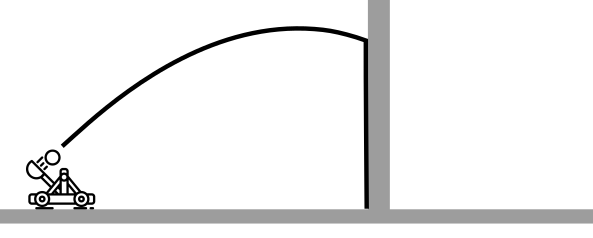
\includegraphics[width=\linewidth]{images/ch6/ballistic.png}
    \end{subfigure}
    \begin{subfigure}[t]{0.3\linewidth}
        \centering
        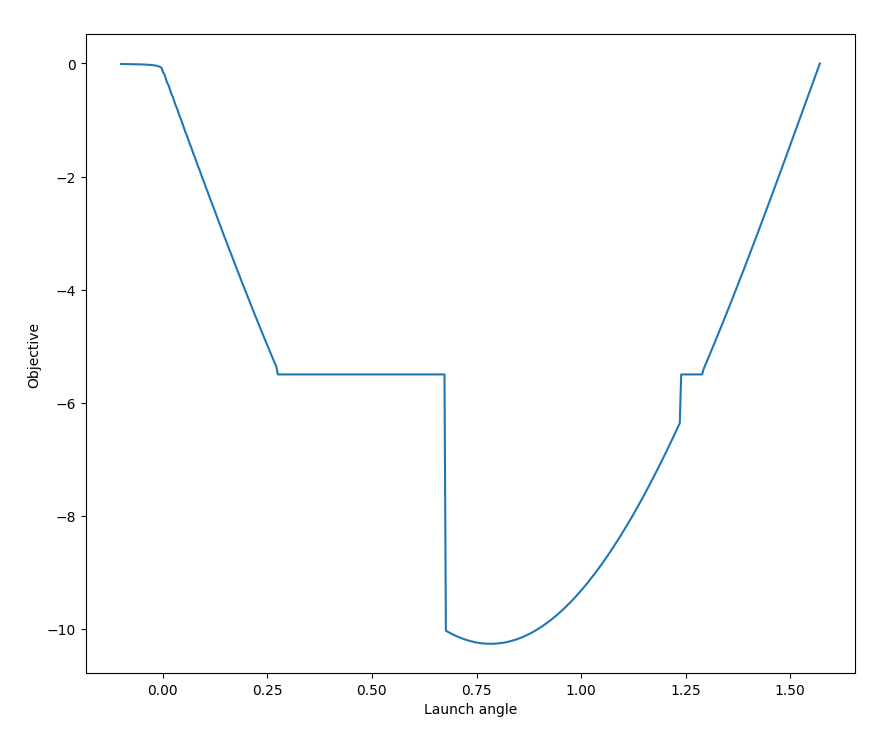
\includegraphics[width=\linewidth]{images/ch6/ballistic_cost.png}
    \end{subfigure}%
    \caption{Left: the ballistic optimization problem from~\cite{suhDifferentiableSimulatorsGive2022a}. Right: the corresponding cost landscape.}
    \label{ch6:fig:ballistic}
\end{figure}

\begin{figure}[tb]
    \centering
    \begin{subfigure}[t]{0.24\linewidth}
        \centering
        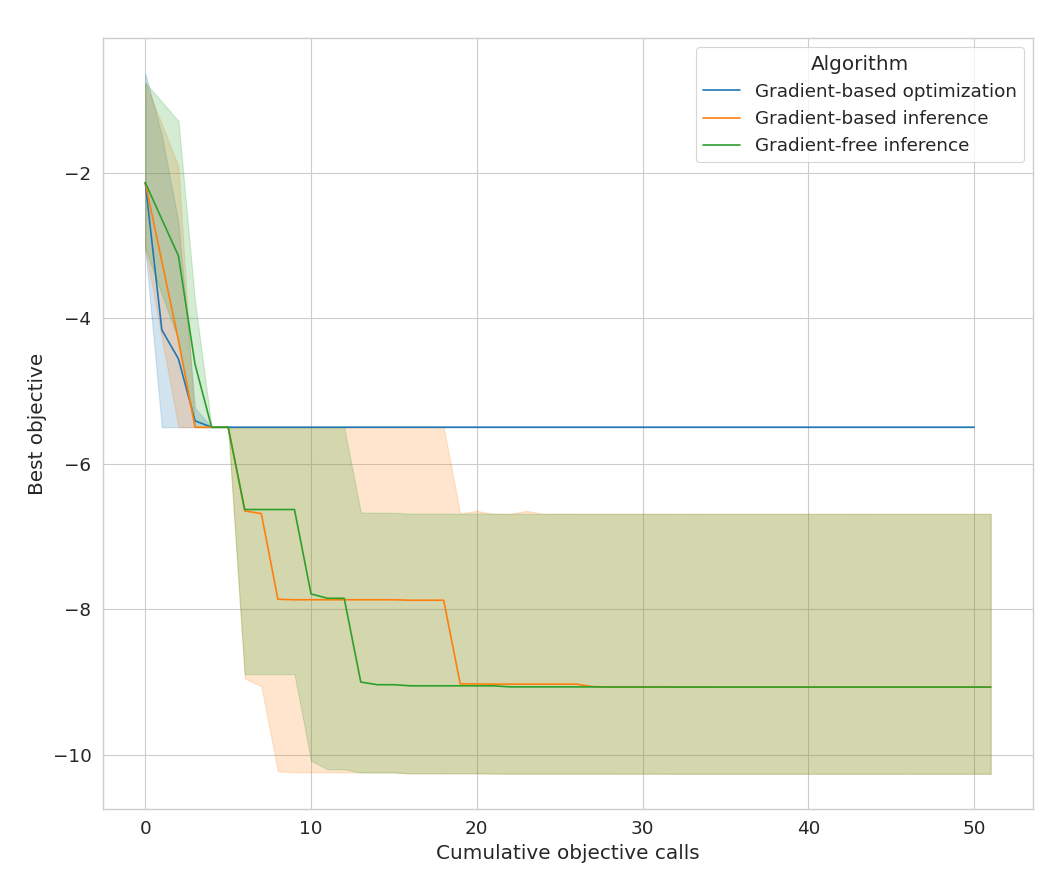
\includegraphics[width=\linewidth]{images/ch6/ballistic_1.png}
    \end{subfigure}
    \begin{subfigure}[t]{0.24\linewidth}
        \centering
        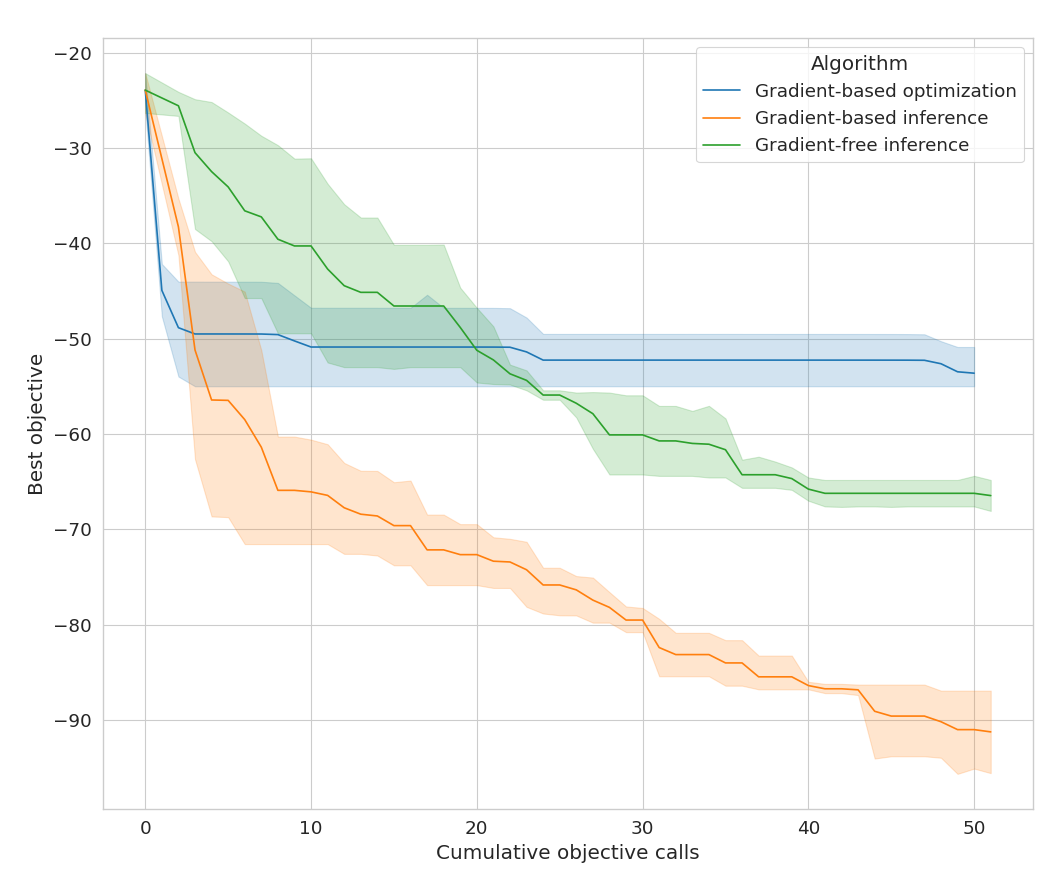
\includegraphics[width=\linewidth]{images/ch6/ballistic_10.png}
    \end{subfigure}
    \begin{subfigure}[t]{0.24\linewidth}
        \centering
        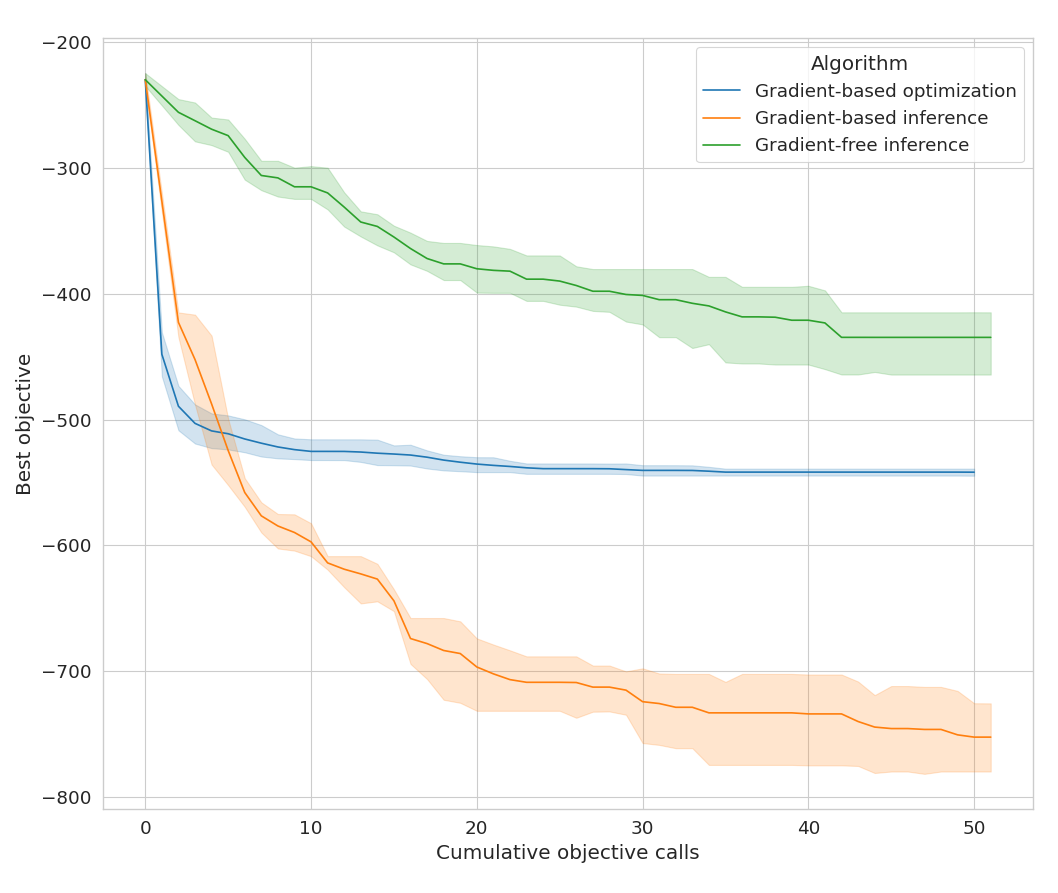
\includegraphics[width=\linewidth]{images/ch6/ballistic_100.png}
    \end{subfigure}
    \begin{subfigure}[t]{0.24\linewidth}
        \centering
        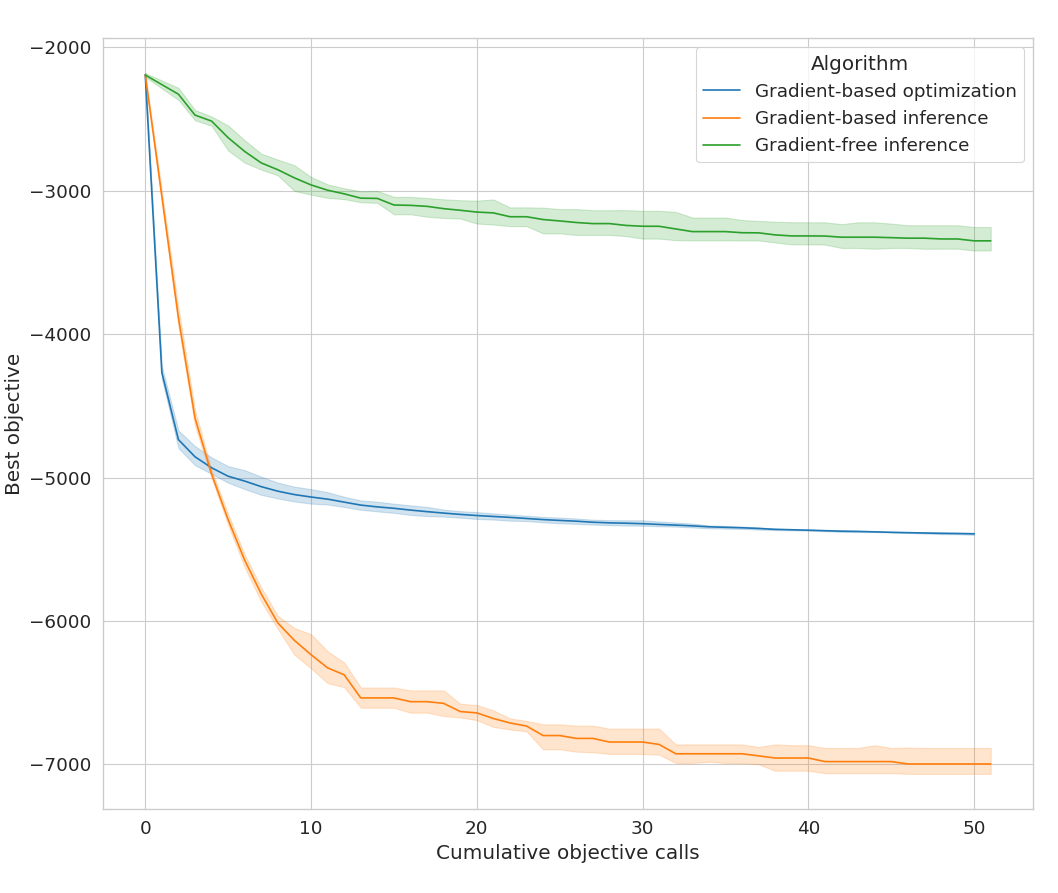
\includegraphics[width=\linewidth]{images/ch6/ballistic_1000.png}
    \end{subfigure}
    \caption{Convergence of gradient-based optimization (gradient descent), gradient-based inference (MALA), and gradient-free inference (RMH) on the ballistic cost landscape from Fig.~\ref{ch6:fig:toy_example}, showing how the inference methods are robust to flat and discontinuous regions of the cost function, and how gradient-based methods excel on high-dimensional problems. From left to right: 1-, 10-, 100-, and 1000-dimensional versions of the problem.}
    \label{ch6:fig:ballistic_convergence}
\end{figure}

\subsection{Sampling and repairing diverse failure modes}

Now that we have motivated the switch from optimization to inference, we will reframe the verification and verification-guided design problems in~\eqref{ch5:eq:verification} and~\eqref{ch5:eq:verification_guided_design_minmax} as inference problems, then demonstrate how we can used gradient-accelerated MCMC sampling (i.e. MALA) to efficiently sample diverse failure modes.

Recall that verification, or \textit{failure prediction}, entails finding exogenous parameters $y^*$ that, for some given $x$, lead to a high cost. To ensure that the predicted failures are plausible, it is important to balance maximizing cost with choosing values for $y^*$ with high prior likelihood. To achieve this balance, we define the metric of \textit{risk-adjusted cost}
\begin{align}
    J_r(x, y) = J \circ S(x, y) + \log p_{y, 0}(y)
\end{align}
where $\circ$ denotes function composition. Failure prediction is thus the problem of finding parameters $y^*$ that lead to a high risk-adjusted cost; moreover, since it is likely that $J_r$ will have multiple local minima with respect to $y$ (i.e. multiple likely failure modes), we wish to sample a set $\set{y^*_1, \ldots, y^*_{n_y}}$ of such high risk-adjusted cost failures. To generate this set, we convert the deterministic optimization problem $y^* = \argmax_y J_r(x, y)$ to the problem of sampling from the unnormalized probability distribution
\begin{align}
    y^* \sim p(y^* | x) \propto p_{y, 0}(y^*) e^{J \circ S(x, y^*)} \label{ch6:eq:prediction_distribution}
\end{align}

Similarly, we can reframe verification-guided design optimization, or \textit{failure mitigation}, as an inference problem. To do so, we assume that, just as there is a prior over exogenous factors $p_{0, y}$, there is also a prior over designs $p_{0, x}$ that reflects the constraints and the designer's prior beliefs about the design space (e.g. assigning zero prior probability to infeasible designs). Failure mitigation then seeks to find design parameters $x^*$ that both have high prior likelihood (thus respecting the designer's prior beliefs about the design space) and results in a low cost across a range of anticipated failure modes. We might frame this as an optimization problem, $x^* = \min_x \left[ \expectation_y J(x, y) + \log p_{x, 0}(x) \right]$ taking the expectation over the likely failure modes distribution~\eqref{ch6:eq:prediction_distribution}, but for the reasons discussed above it is more productive to frame this as a probabilistic sampling problem akin to the one used for failure prediction. To this end, we frame the problem of mitigating a set of failure modes $y^*_1, \ldots, y^*_{n_y}$ as the problem of sampling from the unnormalized distribution
\begin{align}
    x^* \sim p(x^* | y^*_1, \ldots, y^*_{n_y}) \propto p_{x, 0}(x^*) e^{-\sum_{i} J\circ S(x^*, y^*_i) / n_y} \label{ch6:eq:mitigation_distribution}
\end{align}

Using this framework, we can replace the alternating min/max optimization presented in Chapter~\ref{section:local_methods} with a novel adversarial sampling algorithm that alternates between sampling a more robust design and sampling a more likely set of failure modes. This algorithm is presented in Algorithm~\ref{ch6:alg:smc}. It is important to note that this is not the first work to make the connection between MCMC sampling and verification, as~\cite{zhouRoCUSRobotController2021} uses gradient-free sampling to for failure mode prediction and~\cite{sinhaNeuralBridgeSampling2020} uses gradient-based sampling for failure probability analysis, but this is the first work (to our knowledge) that uses sampling to solve adversarial design optimization optimization problems.

Our algorithm (detailed in Algorithm~\ref{ch6:alg:smc}) proceeds in the style of a sequential Monte Carlo algorithm~\cite{chopinIntroductionSequentialMonte2020}. We begin by initializing $n_y$ potential failure modes and $n_x$ candidate designs sampled from their respective prior distributions. Then, in each of $K$ rounds, we first sample $n_x$ new candidate designs from distribution~\eqref{ch6:eq:mitigation_distribution} to mitigate the current set of predicted failure modes. We then select the design that performs best against all currently-predicted failure modes and sample $n_y$ new sets of exogenous parameters (each representing a potential failure mode) from distribution~\eqref{ch6:eq:prediction_distribution} to degrade the performance of the selected design. To sample from distributions~\eqref{ch6:eq:prediction_distribution} and~\eqref{ch6:eq:mitigation_distribution}, we use $n_x$ and $n_y$ parallel executions of the Metropolis-adjusted Langevin algorithm (MALA,~\cite{robertsLangevinDiffusionsMetropolisHastings2002}), a gradient-based MCMC sampling algorithm detailed in Algorithm~\ref{ch6:alg:mala}. In order to handle potential multimodality in the design and failure space, we include optional tempering to interpolate between the prior and target distributions, following~\cite{chopinIntroductionSequentialMonte2020}.

\begin{algorithm}
    \caption{Failure prediction and mitigation using gradient-based sampling\label{ch6:alg:smc}}
    \DontPrintSemicolon
    \KwInput{Design and failure population sizes $n_x$, $n_y$; rounds $K$; substeps $M$; stepsize $\tau$; tempering schedule $\lambda_1, \ldots, \lambda_K$.}
    \KwOutput{Robust design $x^*$ and a set of failures $\set{y_1^*, \ldots, y_{n_y}^*}$ with high risk-adjusted cost.}
    Initialize candidate designs $[x]_0 = \set{x_1, \ldots, x_{n_x}}_0$ sampled from $p_{x, 0}(x)$\;
    Initialize candidate failures $[y]_0 = \set{y_1, \ldots, y_{n_y}}_0$ sampled from $p_{y, 0}(y)$\;
    \For{$i = 1, \ldots, K$}
    {
        $p_{x, i}(x) := p_{x, 0}(x)e^{-\lambda_k / n_y \sum_{y \in [y]_{i-1}} J\circ S(x, y)}$ \Comment{Update designs using predicted failures}\;
        $[x]_i \gets \text{MALA}([x]_{i-1}, M, \tau, p_{x, i})$\;
        $p_{y, i}(y) := p_{y, 0}(y)e^{\lambda_k\min_{x \in [x]_{i-1}} J\circ S(x, y)}$ \Comment{Update failure predictions for new best design}\;
        $[y]_i \gets \text{MALA}([y]_{i-1}, K, \tau, p_{y, i})$\;
    }
    $x^* \gets \argmax_{x \in [x]_{N}} p_{x, i}(x)$ \Comment{Choose best design}\;
    \KwRet{$x^*$, $[y]_K$}
\end{algorithm}

Before moving on to our experimental results, we must discuss a few practical and theoretical aspects of Algorithm~\ref{ch6:alg:smc}. On a theoretical level, the use of MALA (or any MCMC algorithm) to sample from a distribution is sound so long as the resulting Markov chain is ergodic and satisfies detailed balance~\cite{aiama}. The use of Gaussian noise ensures ergodicity (since there is non-zero probability of transitioning between any two feasible states), while the Metropolis-Hastings accept/reject step in Line~\ref{ch6:alg:mala:mh} of Algorithm~\ref{ch6:alg:mala} enforces detailed balance. Unfortunately, there can be a large practical gap between the asymptotic guarantees provided by these conditions and practically acceptable performance.

First, if the target distribution is multimodal and the modes are well-separated, then MCMC algorithms may be slow to move between modes and will yield a biased sampling distribution with any finite number of steps. To mitigate this effect when the target distributions~\eqref{ch6:eq:prediction_distribution} and~\eqref{ch6:eq:mitigation_distribution} are highly multimodal, we include a tempering schedule $0 \leq \lambda_1 \leq \ldots \leq \lambda_K \leq 1$ to interpolate between the prior and target distributions and run multiple MALA instances in parallel from different initial conditions. We find empirically that tempering is not always needed, but we include it for completeness.

The second potential practical challenge arises from the continuity and differentiability (or lack thereof) of the simulator and cost function $J \circ S$. Although MALA remains sound so long as the target distribution is continuously differentiable almost everywhere (i.e. discontinuous or non-differentiable on a set of measure zero), in practice performance may suffer when the target distribution has large discontinuities (it may take an unacceptably long time to accept a move across a discontinuity). As with the problems caused by multimodality, this issues can also be mitigated using of tempering.

The final practical consideration is that although the stochasticity in our sampling-based approach can help us explore the design and failure spaces, we incur a degree of sub-optimality as a result. To reduce this sub-optimality, it is possible to ``quench'' the solution provided by our method by turning off the stochasticity on the last few rounds and executing simple gradient descent (e.g. using MALA for the first 90 rounds and then gradient descent on the last 10 rounds). In practice, we find that quenching can noticeably improve the final cost without compromising the diversity of predicted failure modes.

% Motivation: how to close the design-verification feedback loop.

% Convert min-max optimization from previous section to inference problem.

% Introduce sequential MCMC algorithm for solving this problem.

\subsubsection{Case study: robust generation dispatch for secure power networks}

To see this approach in practice, consider the motivating example of controlling an electric power transmission network subject to failures in transmission lines. Two simple networks (the IEEE 14- and 57-node test system) are shown in Fig.~\ref{ch6:fig:networks}. The goal in this problem is to find control inputs (power injection and voltage at each generator, and power demand at each load) that ensure that the voltage seen by each load is stable, even in the event of transmission outages (which we model using a bimodal distribution for the admittance of each line). The simulator models the AC power flow through this network, and the cost function penalizes excessively high or low voltages or any violation of rated generator capacities. More details on this motivating example is provided in the appendix.

Given a transmission network, the so-called \textit{security-constrained optimal power flow problem} (or SCOPF~\cite{capitanescuStateoftheartChallengesFuture2011}) is the problem of scheduling generator setpoints and power demand from loads to minimize the economic cost of generation and ensure that the network operates safely (satisfying voltage and maximum power constraints) in the event of transmission line outages. The design parameters $x = (P_g, |V|_g, P_l, Q_l)$ include the real power injection $P_g$ and AC voltage amplitude $|V|_g$ at each generator in the network and the real and reactive power draws at each load $P_l, Q_l$; all of these parameters are subject to minimum and maximum bounds that we model using a uniform prior distribution $p_{x, 0}$. The exogenous parameters are the state $y_i \in \R$ of each transmission line in the network; the admittance of each line is given by $\sigma(y_i) Y_{i, nom}$ where $\sigma$ is the sigmoid function and $Y_{i, nom}$ is the nominal admittance of the line. The prior distribution $p_{y, 0}$ is an independent Gaussian for each line with a mean chosen so that $\int_{-\infty}^0 p_{y_i, 0}(y_i) dy_i$ is equal to the likelihood of any individual line failing (e.g. as specified by the manufacturer; we use $0.05$ in our experiments). The simulator $S$ solves the nonlinear AC power flow equations~\cite{cainHistoryOptimalPower2012} to determine the state of the network, and the cost function combines the economic cost of generation $c_g$ (a quadratic function of $P_g, P_l, Q_l$) with the total violation of constraints on generator capacities, load requirements, and voltage amplitudes:
\begin{align}
    J = & c_g + v(P_g, P_{g, min}, P_{g, max}) + v(Q_g, Q_{g, min}, Q_{g, max}) \\
        & + v(P_l, P_{l, min}, P_{l, max}) + v(Q_l, Q_{l, min}, Q_{l, max})     \\
        & + v(|V|, |V|_{min}, |V|_{max}) \label{eq:scopf_cost}
\end{align}
where $v(x, x_{min}, x_{max}) = L\pn{[x - x_{max}]_+ + [x_{min} - x]_+}$, $L$ is a penalty coefficient ($L=100$ in our experiments), and $[\circ]_+ = \max(\circ, 0)$ is a hinge loss.

Efficient solutions to SCOPF are the subject of active research~\cite{capitanescuStateoftheartChallengesFuture2011} and an ongoing competition run by the U.S. Department of Energy~\cite{GridOptimizationCompetition}. In addition to its potential economic and environmental impact~\cite{cainHistoryOptimalPower2012}, SCOPF is also a useful benchmark problem for 3 reasons: 1) it is highly non-convex, 2) it has a large space of possible failures, and 3) it can be applied to networks of different sizes to test an algorithm's scalability. In our case, the 14-bus network has 32 design parameters and 20 exogenous parameters, while the 57-bus network has 98 design parameters and 80 exogenous parameters.

\begin{figure}[tb]
    \centering
    \begin{subfigure}[t]{0.4\linewidth}
        \centering
        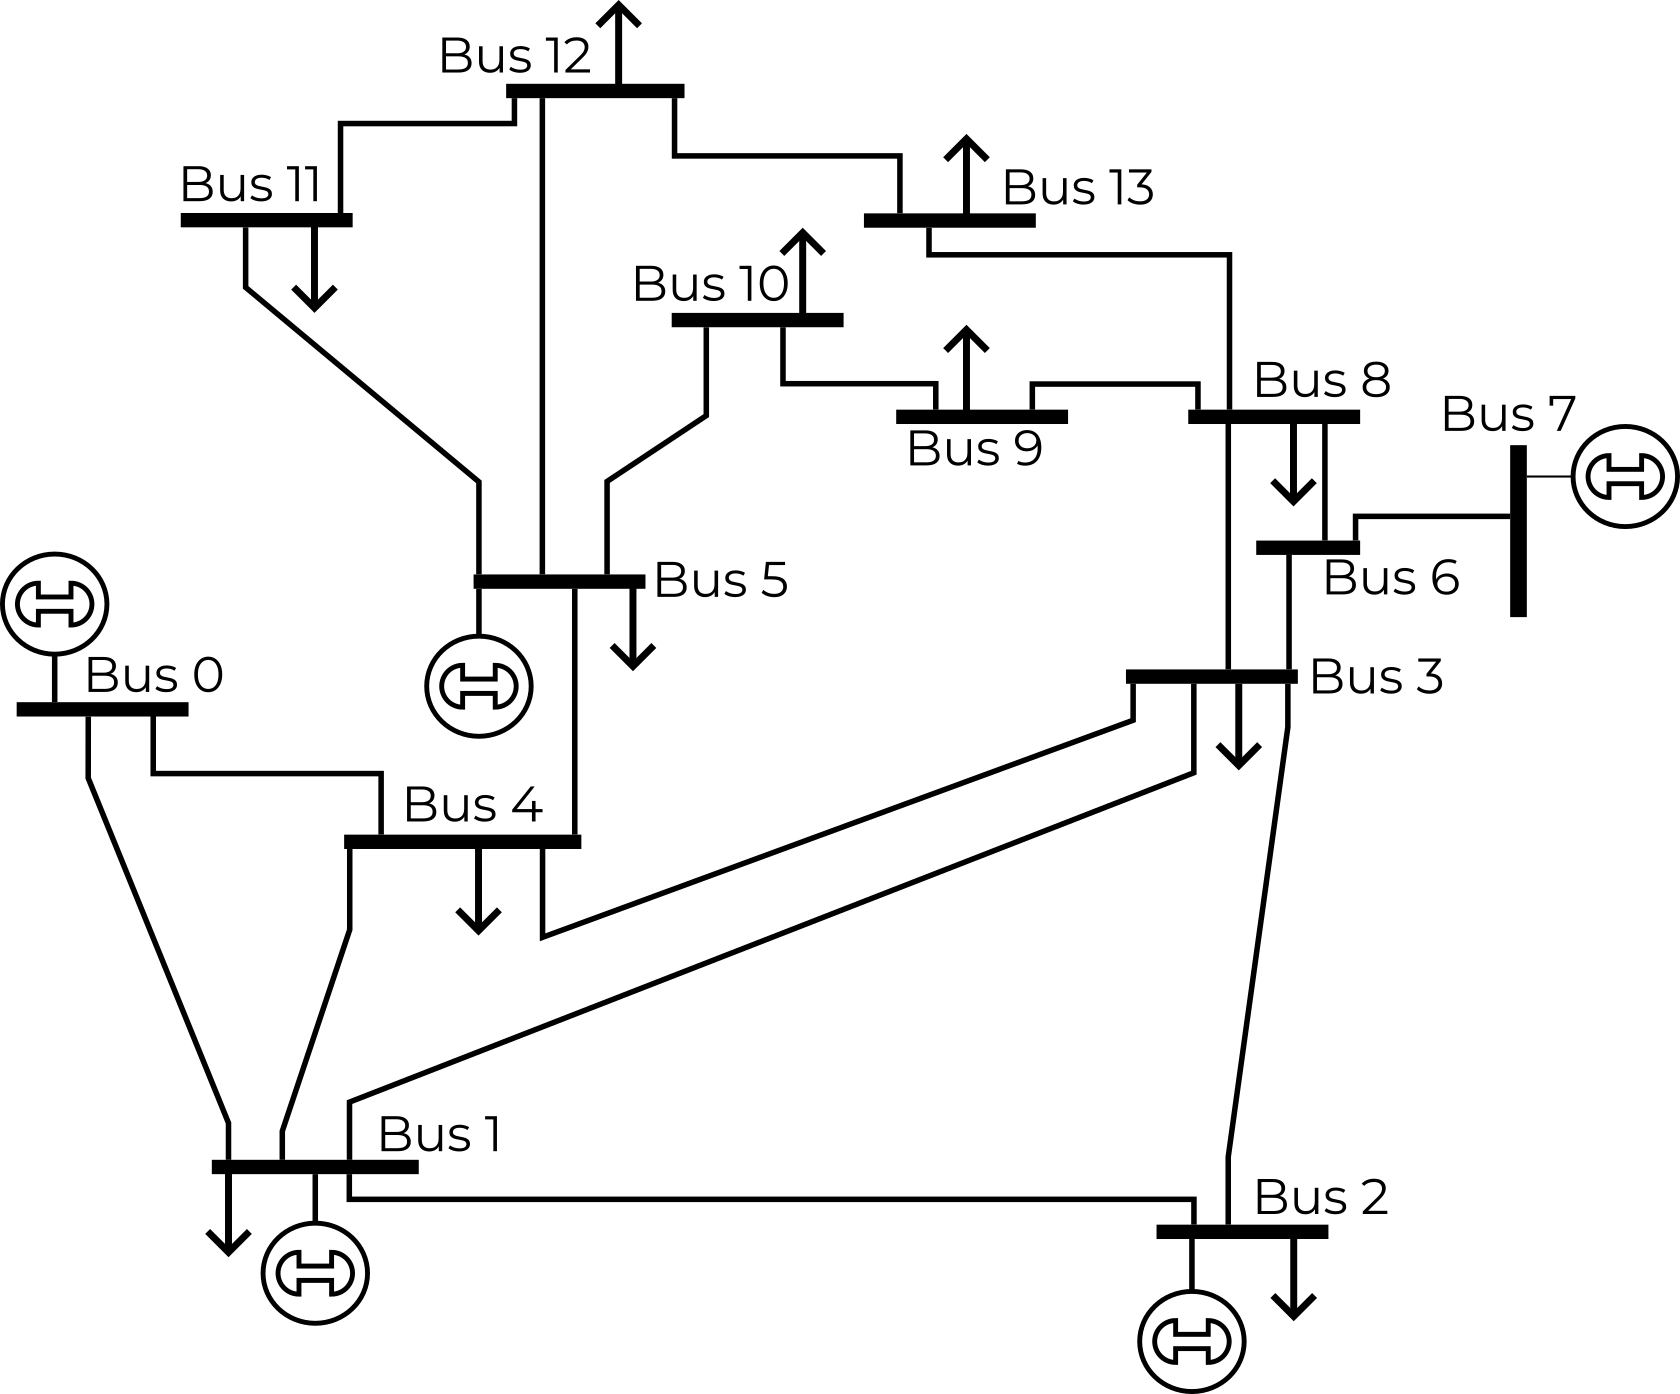
\includegraphics[width=\linewidth]{images/ch6/base_14_bus.png}
    \end{subfigure}
    \begin{subfigure}[t]{0.4\linewidth}
        \centering
        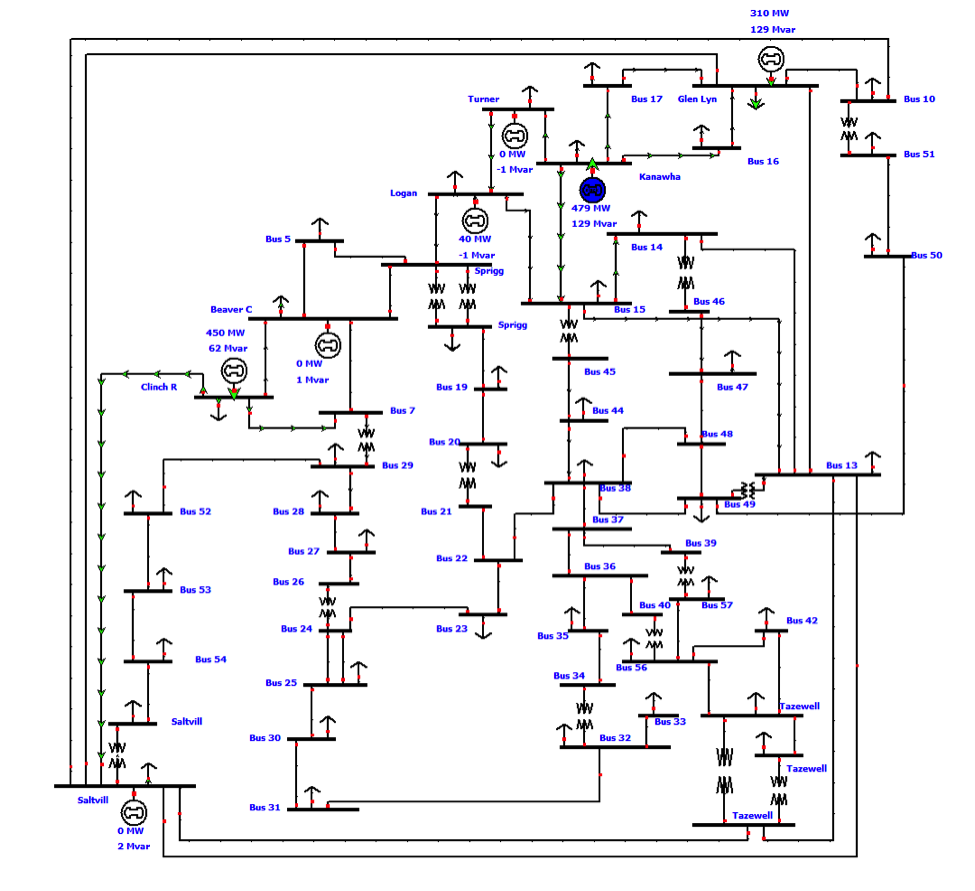
\includegraphics[width=\linewidth]{images/ch6/IEEE57.png}
    \end{subfigure}%
    \caption{Example 14- and 57-bus electricity transmission networks~\cite{illinoiscenterforasmarterelectricgridIEEE57BusSystem}.}
    \label{ch6:fig:networks}
\end{figure}

We can compare our approach quantitatively with the following baselines. \textbf{GD}: solving the adversarial optimization problem $\min_x \max_y J_r(x, y)$ by alternating between optimizing a population of $n_x$ designs and $n_y$ failure modes using local gradient descent. GD is analogous to the methods proposed in~\cite{dontiAdversariallyRobustLearning2021} and in the work in the previous chapter~\cite{dawsonRobustCounterexampleguidedOptimization2022}, modified to provide a fair comparison by using populations of design and exogenous parameters rather than single examples (we intend this baseline to also be representative of a broad class of gradient-based falsifiers~\cite{xuAdversarialAttacksDefenses2020}). \textbf{RMH}: implements Alg.~\ref{ch6:alg:smc} using gradient-free Metropolis-Hastings MCMC with a Gaussian kernel instead of MALA. This baseline represents the straightforward extension of gradient-free failure prediction techniques like ROCUS~\cite{zhouRoCUSRobotController2021} to solve the mitigation problem as well. In addition to these benchmarks, we also include \textbf{GD-NoAdv} to demonstrate what happens when we run \textbf{GD} without updating the exogenous parameters. GD-NoAdv does not represent the state of the art but instead illustrates the benefit of intelligently predicting failure modes rather than relying on vanilla domain randomization.

We implement our method and all baselines in Python using the JAX framework for automatic differentiation and just-in-time compilation. Experiments were run on a laptop with 8 GB of RAM, an 8-core Intel i7-865U CPU running at \SI{1.8}{GHz}, and no GPU. To ensure a fair comparison, all techniques are run with the same population sizes $n_x = n_y = 10$ and total sample budget $KM(n_x + n_y) = 2\times 10^4$ ($K = 100$, $M = 10$); this sample budget was chosen to be large enough that all methods converged. After manual tuning, we found that a step size of $\tau = 10^{-2}$ was appropriate for the exogenous parameters, but $\tau = 10^{-6}$ was required for the design parameters to ensure stability of gradient-based methods. We found that tempering was not required for this problem ($\lambda_i = 1$). For our method, we quench during the final 10 rounds.

We will first compare these methods based on the quality of the solutions they produce, and then on the the speed with which they converge to an optimized design.

\paragraph{Solution quality} To compare the quality of these methods' solutions, we use each method to optimize $n_x = 10$ candidate designs and predict $n_y=10$ failure modes with high risk-adjusted cost. We then select the design that achieves the highest likelihood according to Eq.~\eqref{ch6:eq:mitigation_distribution}, then use one additional round to sample new failure modes that attack the chosen design. The maximum cost across these final predicted failure modes provides a measure of each algorithm's confidence in its solution. We then compare the performance on these predicted failure modes to the maximum cost observed on a test set of $10^6$ exogenous parameters sampled randomly from the prior $p_{y, 0}$. Fig.~\ref{ch6:fig:14_bus_comparison} (top) shows the predicted and observed costs for each method on the IEEE 14-bus test case. The prediction-and-mitigation process took \SI{30.5}{s} for GD-NoAdv, \SI{61.5}{s} for GD, \SI{111.5}{s} for RMH, and \SI{141.7}{s} for our method (including the cost of JAX just-in-time compilation).

\begin{figure}[tb]
    \centering
    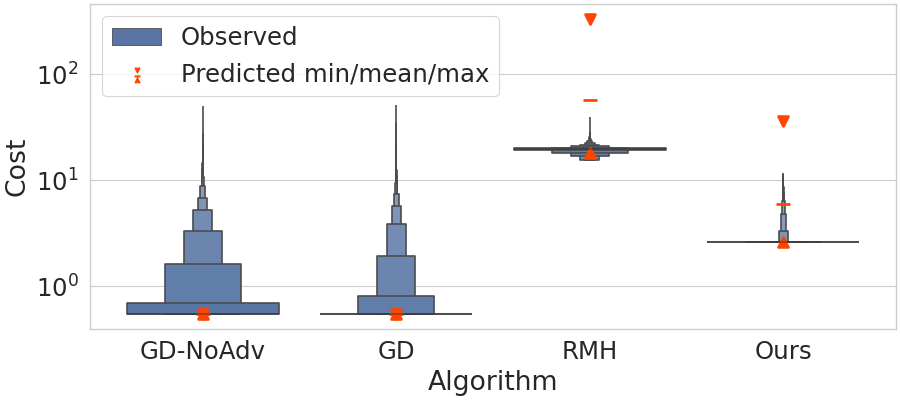
\includegraphics[width=0.45\linewidth]{images/ch6/14_bus_comparison.png}
    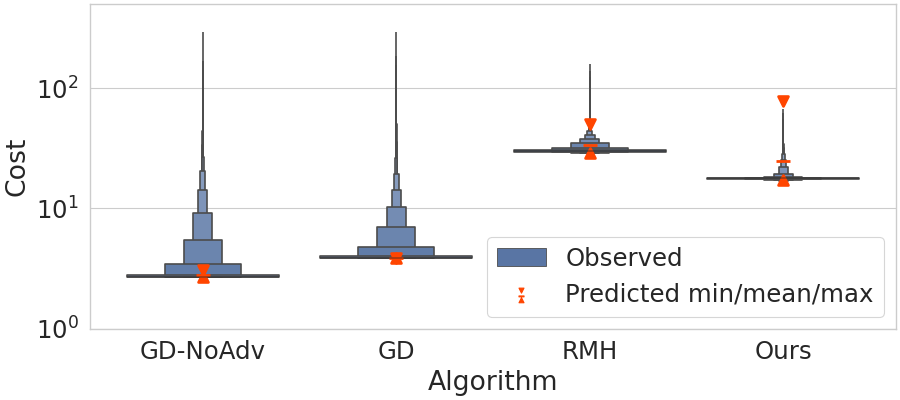
\includegraphics[width=0.45\linewidth]{images/ch6/57_bus_comparison.png}
    \caption{Comparison of our method with baselines for failure prediction and mitigation on a 14-bus (top) and 57-bus (bottom) power transmission network. Red markers show the maximum, mean, and minimum-cost failure modes predicted by each method after optimizing the design, while the box plot shows the distribution of costs on a test set of $10^6$ random failures. Our method not only successfully predicts failure modes that match the range of the empirical distribution, but it also finds a low-cost solution that is more robust than those found by other methods.}
    \label{ch6:fig:14_bus_comparison}
\end{figure}

We can assess these methods in two ways: by the quality of the optimized design and by the quality of the predicted failure cases. The two optimization-based methods, GD and GD-NoAdv, find solutions with the lowest best-case cost, but their solutions are not robust. Not only do these methods find solutions that are susceptible to a heavy tail of failures, but they are overconfident and fail to predict those failures (instead predicting that all 10 candidate failures will be successfully mitigated). In contrast, RMH is not overconfident (it successfully predicts failure modes that match the range of the empirical failure distribution), but it finds a solution that is 10 times costlier than that found by our method. Only our proposed method is able to find a robust, low-cost solution without being overconfident.

Once we have a robust design optimized using our method, we can examine the predicted failure modes to understand the remaining ways in which our design might fail. Of the 10 predicted failure modes, 4 include attacks on the transmission line connecting the generator at bus 7 to the rest of the network (this was the most commonly attacked line). Interestingly, of these 4 attacks, only one (shown in Fig.~\ref{ch6:fig:predicted_failure_modes}) is able to cause a violation of the voltage stability constraints. It is only by fully disconnecting the generator at bus 7 (dotted red line) and partially impairing the line between buses 1 and 4 (solid red; $15\%$ impairment) that we see the voltage drop at several buses (shown in orange). This information about potential failure modes can be very useful to system designers; in this example, the designer may choose to focus monitoring and infrastructure hardening efforts on the two affected lines.

\begin{figure}[tb]
    \centering
    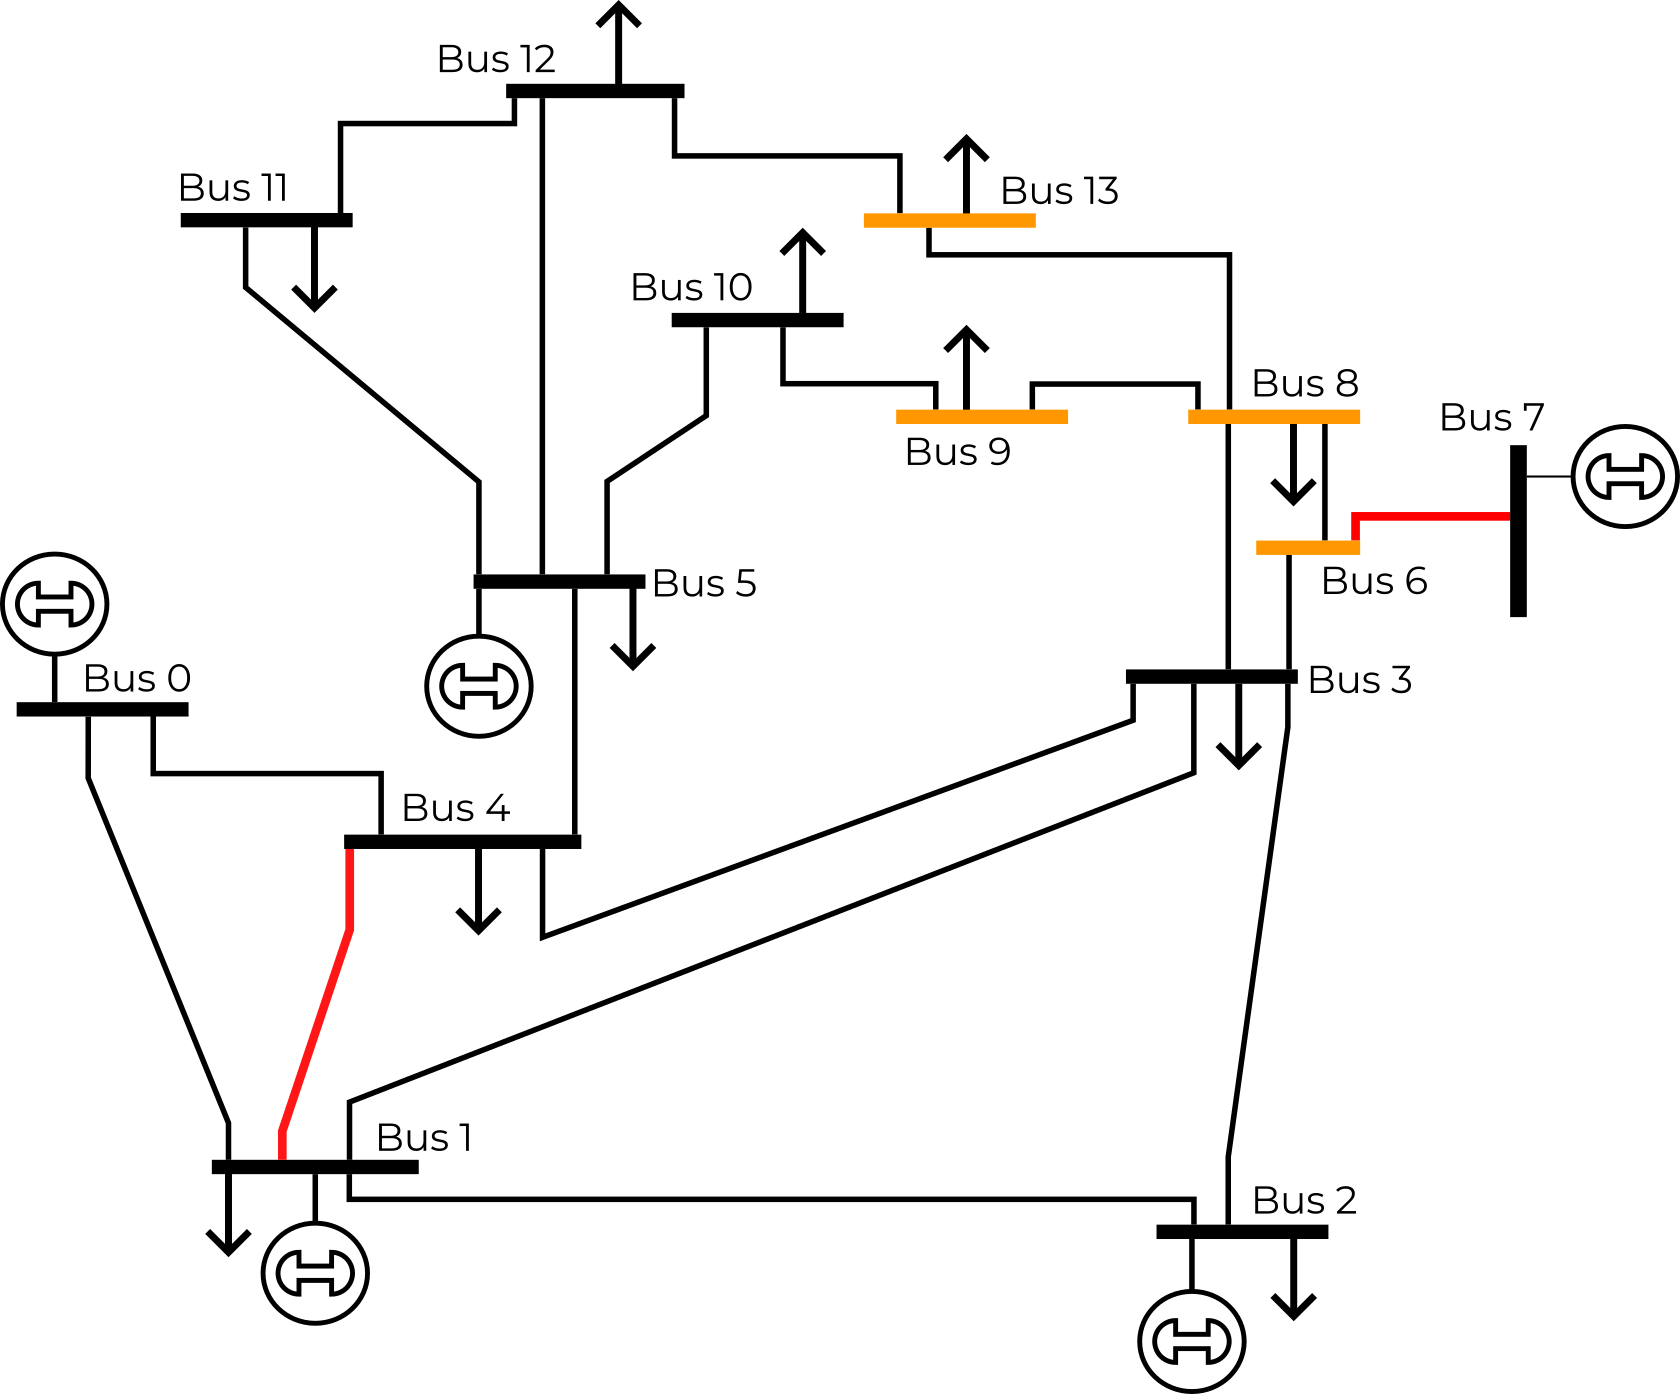
\includegraphics[width=0.4\linewidth]{images/ch6/predicted_failure_modes.png}
    \caption{The only predicted failure modes (of 10 candidates) that causes violation of voltage constraints on the 14-bus transmission network, using the optimized design found using our method. Fully disconnecting the generator at bus 7 (dotted red line) is not enough; other predicted failures include this outage but do not cause a constraint violation. It is only by additionally impairing the line between buses 1 and 4 that the voltage constraint is violated at the buses shown in orange.}
    \label{ch6:fig:predicted_failure_modes}
\end{figure}

To understand the scalability of our approach, we repeat this experiment on a larger 57-bus network with 80 transmission lines. All hyperparameters were the same except for the step size for exogenous parameters, which was reduced to $10^{-3}$. The results are shown in the bottom panel of Fig.~\ref{ch6:fig:14_bus_comparison}; we see that our approach continues to not only find a robust solutions (with a relatively light tail of failures) but also accurately predicts the range of possible failure modes (as opposed to RMH, which does not explore the full failure space in this case). Running GD-NoAdv on this example took \SI{406.2}{s}, GD took \SI{803.4}{s}, RMH took \SI{1002.3}{s}, and our method took \SI{1438.5}{s}.

\paragraph{Convergence rate} From comparing solution quality, there is a clear separation between the sampling- and optimization-based methods, with sampling able to find more robust designs and more accurately cover the range of possible failures (although our gradient-based approach finds higher-quality solutions in both the 14- and 57-node test cases). As a result, a natural question is how these two sampling-based methods compare in how quickly they converge.

To measure the relative convergence rate of RMH and our gradient-based method, we measure the average cost $J$ in each round across all candidate designs $[x]_i$ on a test set of 100 exogenous parameters sampled randomly from the prior distribution. The convergence of this test-set performance as a function of the number of sampling rounds is shown in Fig.~\ref{ch6:fig:training_curves} for both the 14- and 57-bus networks. These results show that our method converges much more quickly than gradient-free RMH, suggesting that the use of automatic differentiation provides a clear advantage.

\begin{figure}[tb]
    \centering
    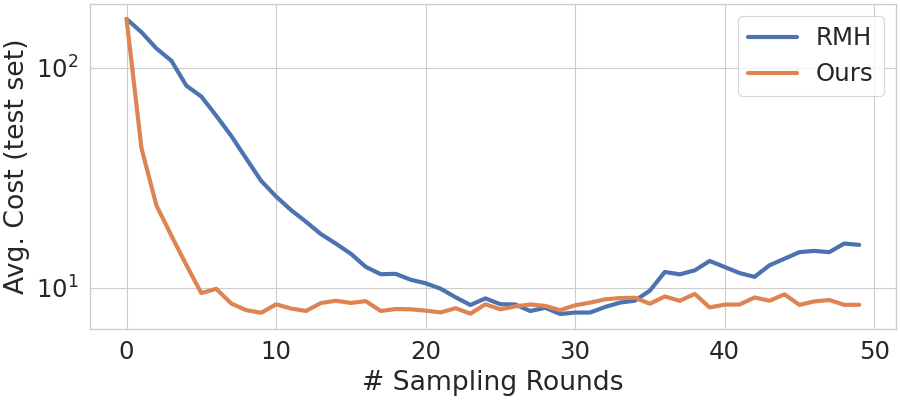
\includegraphics[width=0.45\linewidth]{images/ch6/14_bus_training_curves.png}
    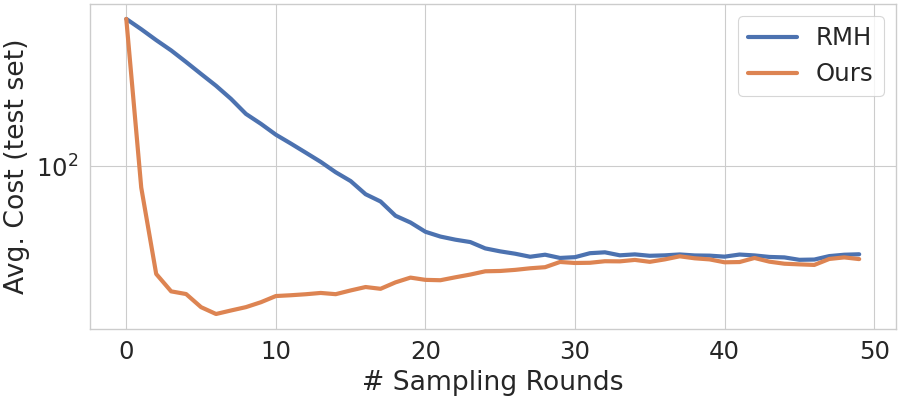
\includegraphics[width=0.45\linewidth]{images/ch6/57_bus_training_curves.png}
    \caption{Comparison of convergence rates of our method and a gradient-free sampling baseline on 14- (top) and 57-bus (bottom) power networks, showing average cost of 10 candidate designs on a test set of 100 random exogenous parameters. Our gradient-based method converges significantly faster than gradient-free RMH. The gradual increase in cost after convergence is likely due to distribution shift between the predicted failure modes and the prior distribution.}
    \label{ch6:fig:training_curves}
\end{figure}

\subsubsection{Case study: Vision-based control}

We have also applied our approach to problems involving visual feedback, implementing a differentiable rendering engine in JAX and applying the adversarial sampling approach from Algorithm~\ref{ch6:alg:smc}. We define a range of vision-based control tasks, from autonomous vehicle control to grasp keypoint prediction, as shown in Fig.~\ref{ch6:fig:vision_scenarios}. For each of these scenarios, a policy was pretrained using a traditional method (either PPO or behavior cloning), and then we apply our method to identify and repair failure modes.

Example failures for the drone and autonomous vehicle scenarios are shown on the left in Fig.~\ref{ch6:fig:repairs}, while the repaired policy is shown on the right for each case. We can see that some of the pretrained policies, such as for autonomous driving on a highway, are overly aggressive and prone to failures, while the repaired policy is much safer.

\begin{figure}
    \centering
    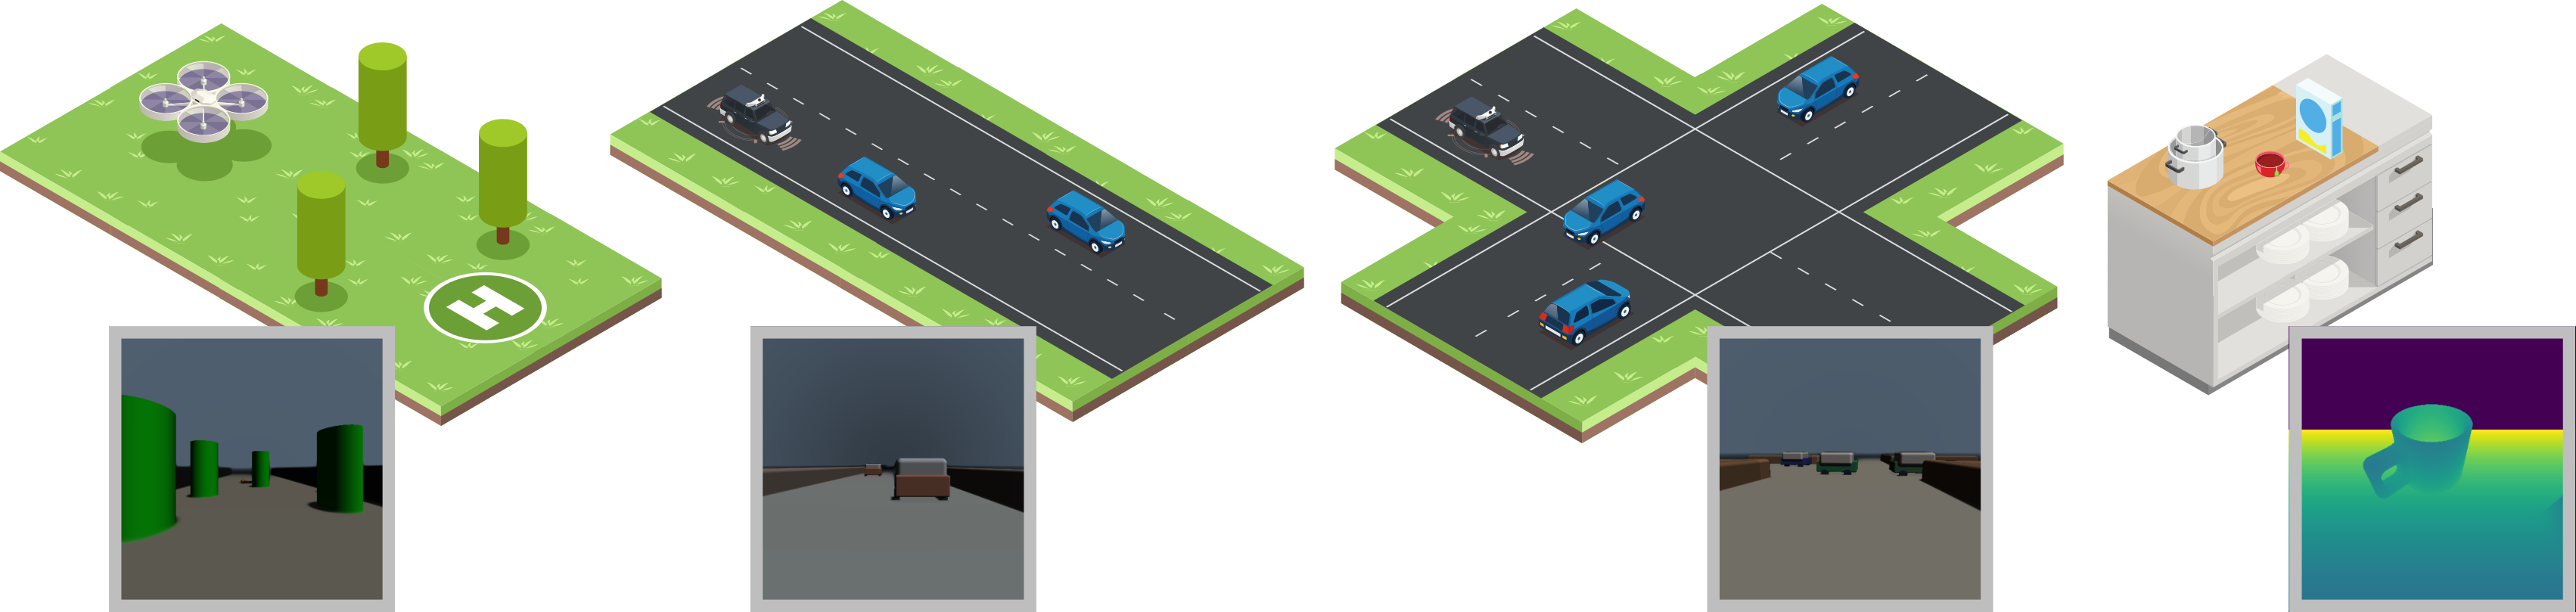
\includegraphics[width=\linewidth]{images/ch6/all_scenarios.png}
    \caption{Environments for drone navigation, AV control, and household object manipulation. Inset: a robot's-eye-view of each scene rendered using our differentiable renderer.}\label{ch6:fig:vision_scenarios}
\end{figure}

\begin{figure}[t]
    \centering
    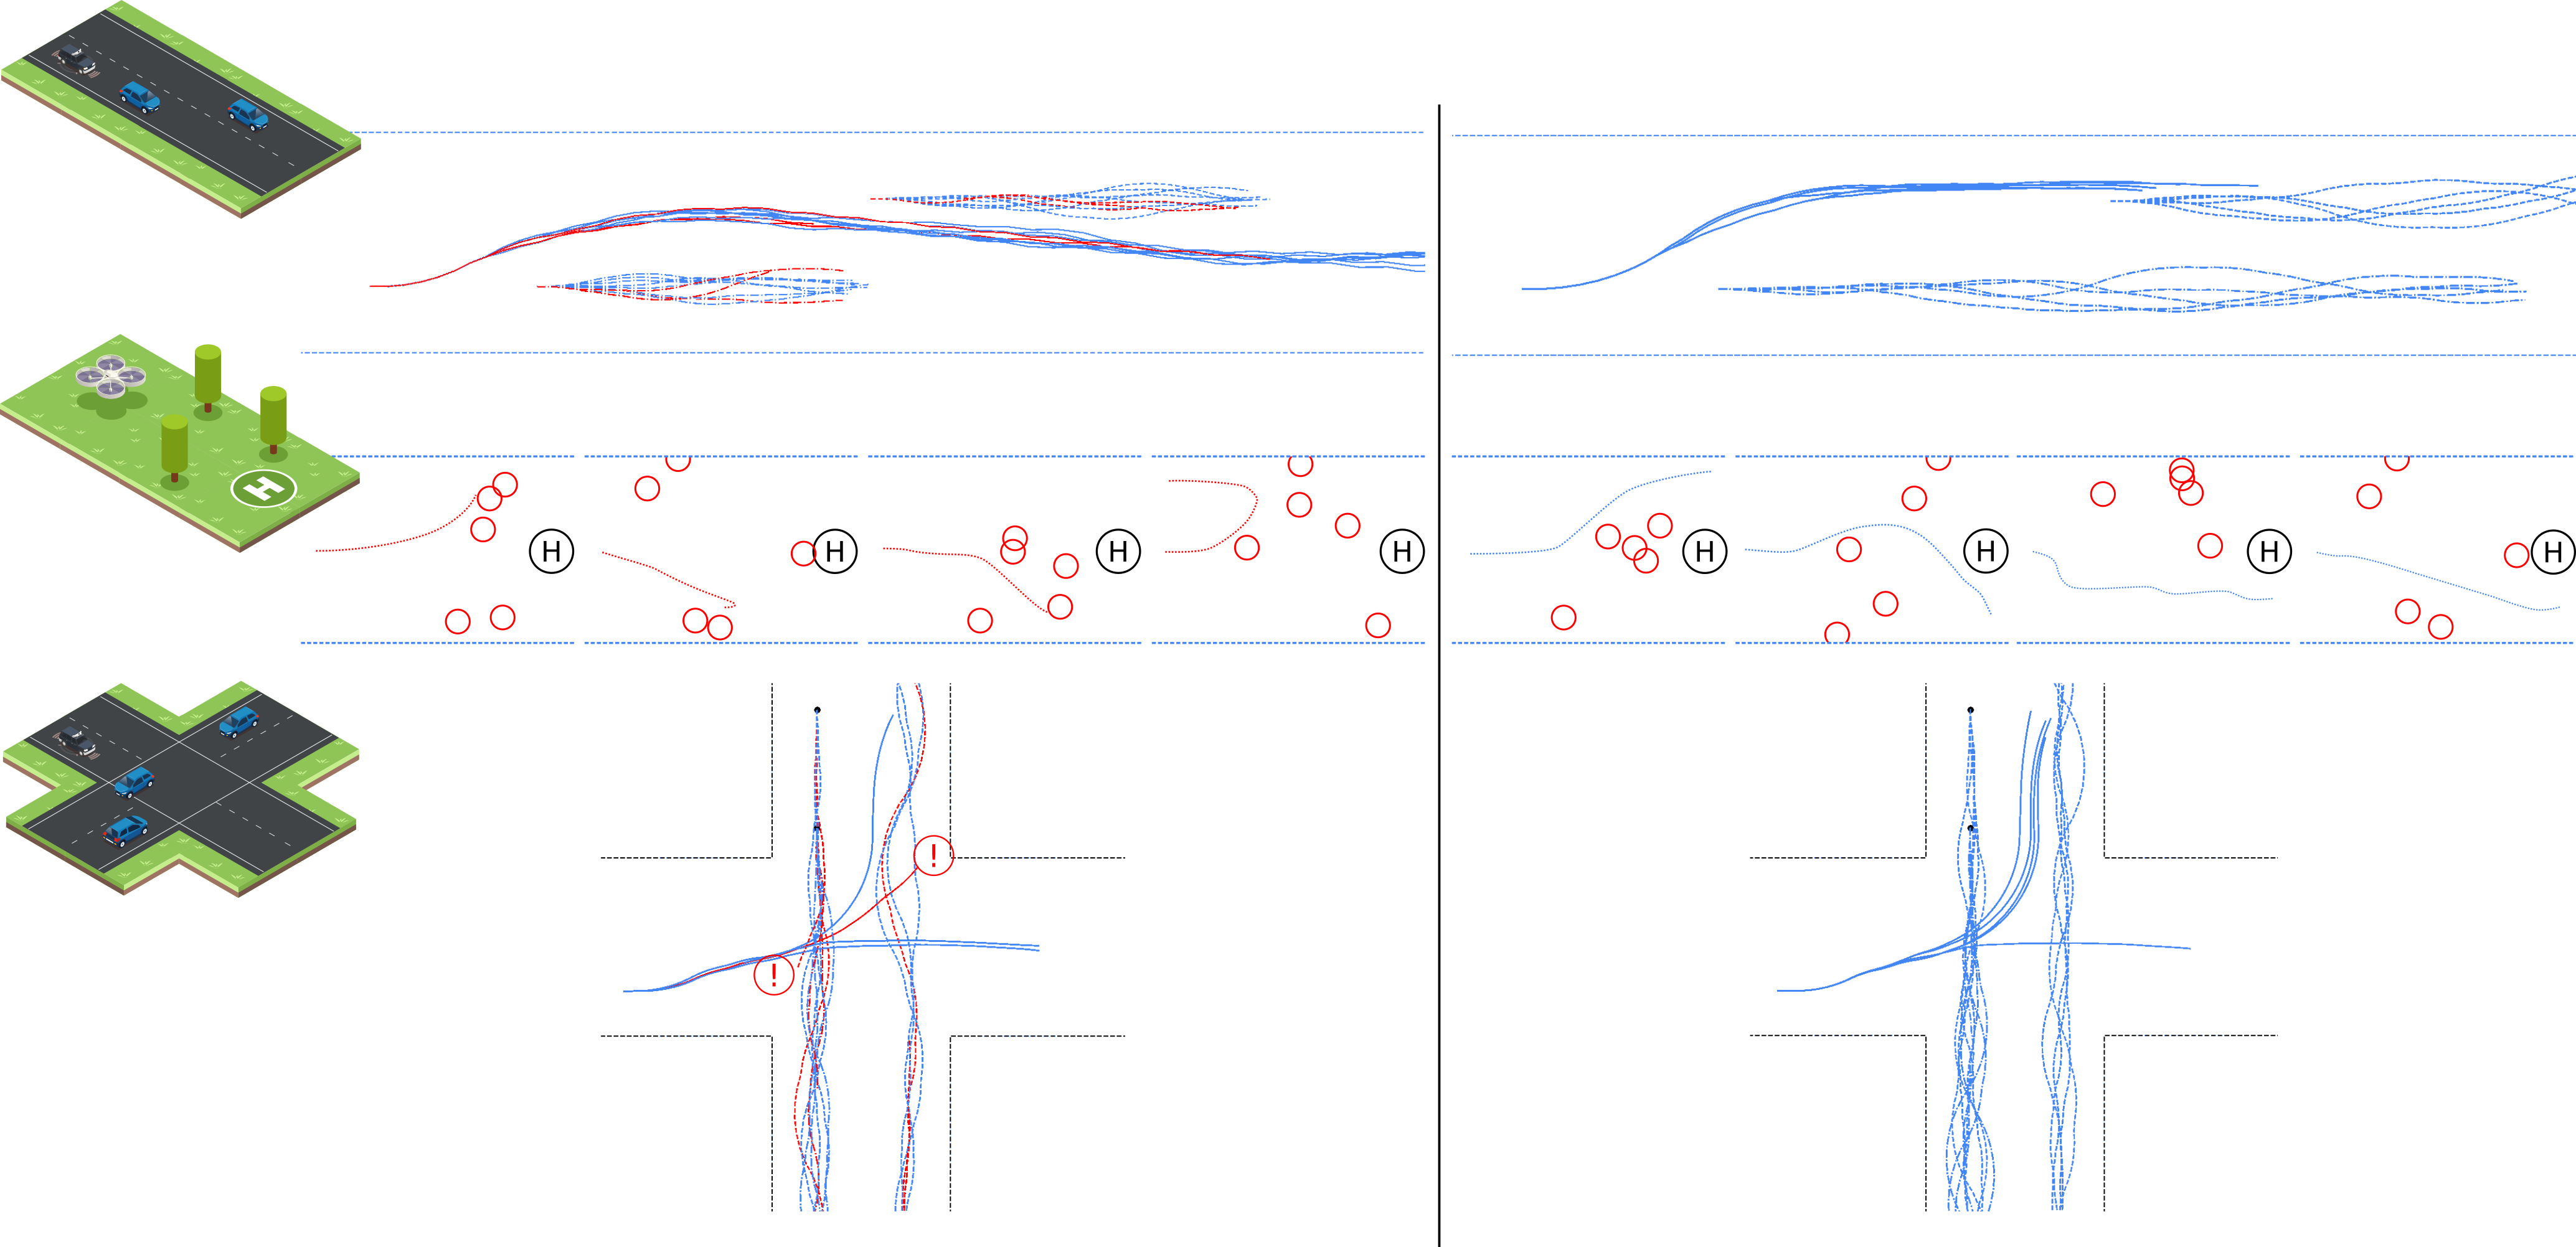
\includegraphics[width=\linewidth]{images/ch6/repairs.png}
    \caption{Examples of failure cases (left) and repaired policies (right) generated using our method.}\label{ch6:fig:repairs}
\end{figure}

% Problem setup

% Research questions relevant to state of the art.

% Results

% How do our results compare to the state of the art? - Highlight overconfidence of gradient-only methods and poor solution quality of gradient-free methods.

\subsection{Discussion \& Limitations}

This chapter has presented the results of ongoing research demonstrating that:

\begin{enumerate}
    \item For problems with multiple local minima and poorly-conditioned gradients, an inference-based approach leads to more robust solution methods than an optimization-based approach.
    \item Optimization-as-Inference problems can be solved using either gradient-based or gradient-free methods, but gradient-based methods (enabled by automatic differentiation) perform much better on higher dimensional problems.
    \item The verification-guided design problem can be solved using a novel adversarial inference algorithm, a gradient-based version of which leads to faster convergence, better coverage of the failure space, and more robust designs.
\end{enumerate}

The results in this chapter, particularly regarding vision-based control, are preliminary; more work is needed to benchmark gradient-free and gradient-based inference methods against optimization methods on a range of robotics problems. In addition, although I have preliminary theoretical results that provide conditions under which gradient-based inference methods will work well (building on the results in~\cite{maSamplingCanBe2019}), more work is required to understand a) what features of a problem are required for this approach to work well (e.g. degree of smoothness, extent of discontinuity, etc.) and b) to develop runtime checks to determine whether a problem is well-suited for gradient-based inference.

%!TEX root = ./main.tex

\section{Future work}\label{section:future_work}

There are three areas of future work I plan to explore in the next year before defending my thesis.

\paragraph{Benchmarking} Chapter~\ref{section:global_methods} includes a number of preliminary results suggesting that gradient-based inference methods perform well on a range of challenging robotics problems, including problems with poorly-conditioned gradients (flat regions and discontinuities). However, it is not yet clear what underlying factors contribute to this performance. In the next year, I will perform a series of experiments to both ablate different aspects of gradient-based inference methods and apply them to problems with different challenging features (including discontinuities, stiff gradients, subgradients, and inaccurate gradients). The goal will be to develop practical guidance for when practicioners can expect gradient-based inference methods to perform well.

Specifically, this research will proceed in four stages:
\begin{enumerate}
    \item Define a suite of state-of-the-art optimization and inference algorithms, including gradient-free and gradient-based methods, including ablations of particular methods.
    \item Define a suite of benchmark problems with the ability to scale aspects like problem dimension, number and extent of discontinuities, number of distinct modes, etc..
    \item Conduct benchmarking experiments to compare the performance of different algorithms on different problems.
    \item Using results from benchmarking, infer practical checks that can be used to determine whether a problem is suitable for gradient-based inference methods, and compile these checks into a software package that can be used by practitioners.
\end{enumerate}

\paragraph{Probabilistic programming} In my work in Chapter~\ref{section:global_methods}, I combine automatic differentiation with gradient-based inference on programs with a specific structure $J(S(x, y))$. The decision to factor out all uncertainty into the inputs $y$ makes easier to apply approximate inference algorithms, but it enforces a fixed topology on the underlying probabilistic graphical model (requiring graphical models with the structure shown on the left in Fig.~\ref{ch7:fig:graphical_models}). This restricted set of structures restricts the expressiveness of the probabilistic model, in particular making it difficult to model interactions between exogenous parameters (as in the example structure shown on the right in Fig.~\ref{ch7:fig:graphical_models}). In the next year, I will explore how to remove this restriction through the use of a fully-features probabilistic programming language such as Gen~\cite{Cusumano-Towner:2019:GGP:3314221.3314642}. Using such a language, it is possible to define programs that make random choices without factoring out the uncertainty (instead, special syntax is used to annotate random choices as they occur in the code).

\begin{figure}[b]
    \centering
    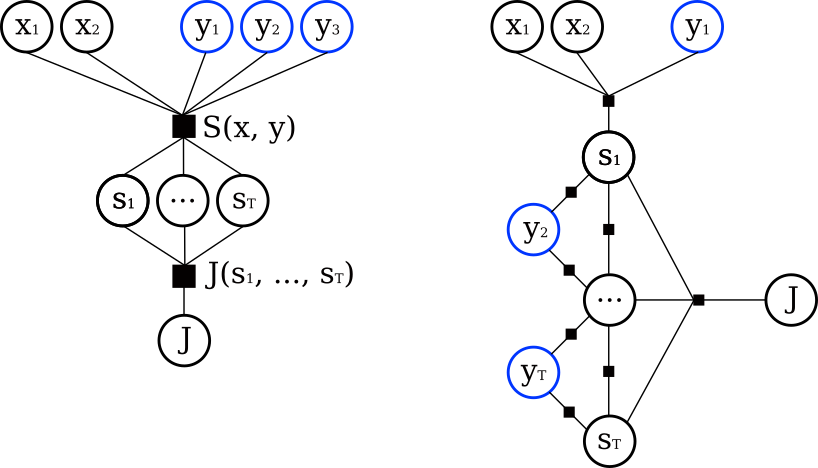
\includegraphics[width=0.8\linewidth]{images/ch7/graphs.png}
    \caption{Left: a factored graphical model in the form supported by the inference methods presented in Chapter~\ref{section:global_methods}, where all random choices (blue circles) are factored out into the exogenous inputs $y$. Right: a graphical model with a more complex structure, where random choices are not factored out and can depend on intermediate states.}
    \label{ch7:fig:graphical_models}
\end{figure}

In particular, this research will explore two distinct questions:
\begin{enumerate}
    \item Can we use probabilistic programming to perform causal analysis of autonomous systems, in particular answering root-cause failure analysis problems? E.g. if a robot fails to complete a task in a particular way, can we use probabilistic programming to infer the most likely cause or causes of the failure?
    \item Can we use probabilistic programming to define inference problems that search over the space of possible program structures? E.g. to search over the space of possible robot limb morphologies, or to search over symbolically-defined control policies? This will involve drawing on recently-developed methods for involutive and reversible-jump MCMC, which have been applied to inference problems with hierarchical models~\cite{cusumano-townerAutomatingInvolutiveMCMC2020}.
\end{enumerate}

% Explain gap between existing approach (reparameterization trick/factor out all randomness into inputs to deterministic function) and probabilistic programming.

% Explain advantages that probprog may have for a design process.

% Formulate specific research goal.

\paragraph{Lessons learned for gradient-free solution methods}

A large part of this thesis is motivated by the ability to introspect program structure (e.g. through automatic differentiation) to improve the performance of design and verification algorithms. Unfortunately, there will always be problems where it is not feasible to perform this introspection; for example, if a simulator relies on proprietary code that is only available in binary form, or if there is simply not enough engineering effort available to port an existing simulator to an AD-compatible library. To handle these cases, in the next year I will explore how to apply the lessons learned from gradient-based design and verification to accelerate gradient-free solution methods, including through the use of gradient estimation and proxy modeling.

The main output of this line of research will be a gradient-free MCMC inference algorithm that uses a combination of proxy modeling and gradient estimation to accelerate convergence to the target distribution. This algorithm will be evaluated on a range of challenging problems, including problems with stiff gradients, discontinuities, and flat regions.

%!TEX root = ./main.tex

\section{Milestones and Program Logistics}\label{section:planning}

\subsection{Classes and Degree Milestones}

Table~\ref{ch8:tab:course_requirements} shows my competed coursework, and Table~\ref{ch8:tab:degree_milestones} shows completed and anticipated degree milestones.

\begin{table}[h]
    \centering
    \caption{My completed coursework, satisfying all academic requirements for the doctoral program. Major: autonomy. Minor: controls.}
    \label{ch8:tab:course_requirements}
    \begin{tabular}{llll}
        Semester    & Class                                             & Req.       & Status    \\ \hline
        Fall 2019   & 16.413 Principles of Autonomy \& Decision Making  & major      & completed \\
        Fall 2019   & 6.255 Optimization Methods                        & major/math & completed \\
        Spring 2020 & 16.412 Cognitive Robotics                         & major      & completed \\
        Spring 2020 & 6.832 Underactuated Robotics                      & minor      & completed \\
        Fall 2020   & 18.385 Nonlinear Dynamics and Chaos               & minor/math & completed \\
        Fall 2020   & 2.160 Identification, Estimation, and Learning    & minor      & completed \\
        Spring 2021 & 16.S398 Formal Methods in Autonomy                & major      & completed \\
        Fall 2021   & 6.843: Robotic Manipulation                       & major      & completed \\
        Fall 2021   & 16.995 Doctoral Research \& Communication Seminar & RPC        & completed
    \end{tabular}
\end{table}

\begin{table}[h]
    \centering
    \caption{Milestones towards my completion of the doctoral degree. Italicized milestones are anticipated.}
    \label{ch8:tab:degree_milestones}
    \begin{tabular}{rl}
        Fall 2019 (September)       & Began studies at MIT                           \\
        Fall 2020 (December)        & Field evaluation complete                      \\
        Spring 2021 (May)           & Masters thesis submitted                       \\
        Fall 2022 (September)       & Committee meeting \#1                          \\
        Summer 2023 (June)          & Commitee meeting \#2 and thesis proposal       \\
        \textit{Fall 2023}          & \textit{Committee meeting \#3}                 \\
        \textit{Spring 2024}        & \textit{Committee meeting \#4 and green light} \\
        \textit{Spring/Summer 2024} & \textit{Thesis defense}
    \end{tabular}
\end{table}

\subsection{Research Schedule}

My thesis research will proceed in stages, as outlined below.

Spring 2022
\begin{enumerate}
    \item Certifiable robot design optimization using differentiable programming
          \begin{enumerate}
              \item Develop design optimization tool using automatic differentiation
              \item Develop statistical robustness certification tool based on extremal types theorem
              \item Hardware deployment
              \item Accepted to RSS 2022
          \end{enumerate}
    \item Robust counterexample-guided optimization with temporal logic specifications
          \begin{enumerate}
              \item Define two-player zero-sum game between the designer and the verifier
              \item Incorporate counterexamples from the verifier to guide robust design optimization
              \item Use differentiable signal temporal logic for complex task specification
              \item Submitted to IROS 2022
          \end{enumerate}
\end{enumerate}

Fall/Winter 2022
\begin{enumerate}
    \item Improving design optimization and verification through automated failure mode discovery
          \begin{enumerate}
              \item Use differentiable programming and sequential MCMC to discover a diverse set of possible failure modes.
              \item Use counterexamples from all failure modes to guide robust design optimization
          \end{enumerate}
\end{enumerate}

Spring 2023
\begin{enumerate}
    \item Extend failure mode prediction and mitigation framework to challenging new problem domains, including:
          \begin{enumerate}
              \item Perception-in-the-loop controllers, through the use of differentiable rendering,
              \item Deep neural network controllers.
          \end{enumerate}
\end{enumerate}

\textit{Fall 2023}
\begin{enumerate}
    \item Develop MCMC-based algorithm for safety verification and optimization of systems with discrete structure (e.g. involutive MCMC for robot manipulators with variaible morphologies).
    \item Write thesis
\end{enumerate}

\textit{Spring 2024}
\begin{enumerate}
    \item Write thesis
    \item Defend thesis and graduate
\end{enumerate}


%---------------------------------------------------------------------------------------------%
% Bibliography
%---------------------------------------------------------------------------------------------%
\newpage

%-----------------------%
% automatic bib entries %
%-----------------------%
% enter your bibliographies using a .bib file
% for most formats, the unsrt argument (unsorted) will list the bibliographies as cited in the 
% text, rather than sorting them alphabetically. For the \bibliography entries, much like the 
% \graphicspath entries, each relative file directory is separated by a comma, no space,
% followed by the .bib file name, without the .bib extension
\bibliographystyle{apalike}
\bibliography{main}
% example: \bibliography{../bib/bib_example,../bib/bib_example2,../bib/bib_example3}


% %---------------------------------------------------------------------------------------------%
% % Appendix
% %---------------------------------------------------------------------------------------------%
\newpage
\appendix
\section{Appendix: Details on local methods}

\subsection{AD-enabled design optimization}

To develop a general-purpose, efficient, and robust design optimization framework for autonomous systems, we must address three main challenges. First, how can we ensure that the system is \textit{flexible}, not requiring large amounts of work to specialize the framework to particular application domains. Second, how can we incorporate \textit{robustness} into the design optimization process, to minimize the sensitivity of the optimized design to variation in the exogenous parameters. Finally, how can we achieve both of these goals \textit{efficiently}, making use of gradients wherever possible to accelerate the search for high-performing designs.

\paragraph{Flexibility} Most robots are composed of many interacting subsystems, and different subsystems are typically modeled using different levels of abstraction. Although some tools may aid in designing certain subsystems (e.g. Simulink for controllers, SolidWorks for hardware), these tools cover only a small part of the overall robotics design problem, which includes sensing, actuation, perception, navigation, control, and decision-making subsystems. Since few robotic systems are exactly alike, an effective design tool must allow the user to select an appropriate level of abstraction for the problem at hand.

When it comes to managing complexity in a general-purpose design framework, programming languages are a natural tool. They allow users (i.e. programmers) to define precisely which abstractions are appropriate for any given application (e.g. by defining appropriate class hierarchies and function interfaces) without sacrificing generality. To take advantage of this expressivity, we can view engineering designs as programs that define the behavior of the system given suitable choices for design structure and parameters. We can then use automatic differentiation to derive gradients connecting these parameters to the system's behavior and optimize accordingly. This view is inspired by recent work in 3D design optimization~\cite{cascaval2021differentiable}, aircraft design~\cite{sharpe_thesis}, and machine learning~\cite{paszkePyTorchImperativeStyle2019,jax2018github}.

\paragraph{Robustness} Robots operate in dynamic environments that cannot be fully specified \textit{a priori}, and nonlinear interactions between the robot and its environment can make this uncertainty difficult to quantify. Nevertheless, we must account for this uncertainty during the design process and ensure that our designs perform robustly.

Due to this uncertainty, simply minimizing the expected value of the cost $\expectation_{y \sim \cY} \big[ J\pn{S\pn{x, y}} \big]$ can lead to myopic behavior where exceptional performance for some values of $y$ compensates for poor performance on other values; this is related to the phenomenon of ``reward hacking'' in reinforcement learning~\cite{amodei2016_ai_safety}. Ideally, we would like our designs to be robust to variations in exogenous parameters: changing $y$ should not cause the performance to change much. We can include this requirement as a heuristic by penalizing the variance of $J$. Intuitively, this heuristic ``smooths'' the cost function with respect to the exogenous parameters: regions of high variance (containing sharp local minima) are penalized, while regions of low variance are rewarded. This heuristic leads us to the \textit{variance-regularized robust design optimization problem}:
\begin{subequations}\label{app:ch5:eq:design_optimization_nlp_generic}
    \begin{align}
        \min_{x \in \cX} & \quad \expectation_{y \sim \cY} \Big[ J\circ S\pn{x, y} \Big] + \lambda \rm{Var}_{y\sim\cY}\Big[ J\circ S\pn{x, y} \Big] \label{app:ch5:eq:design_optimization_objective_generic}
    \end{align}
\end{subequations}
Practically, we replace the expectation and variance with unbiased estimates over $N$ samples $y_i \sim \cY, i=1,\ldots,N$.
\begin{subequations}\label{app:ch5:eq:design_optimization_nlp}
    \begin{align}
        \min_{x \in \cX} & \quad \frac{1}{N}\sum_{i=1}^{N} \Big[J\circ S\pn{x, y_i}\Big] + \lambda \left[ \frac{\sum_{i=1}^N \pn{J\circ S\pn{x, y_i}}^2}{N-1} - \frac{\pn{\sum_{i=1}^N J\circ S\pn{x, y_i}}^2}{(N-1)N} \right] \label{app:ch5:eq:design_optimization_objective}
    \end{align}
\end{subequations}

\paragraph{Efficiency} Of course, this Monte-Carlo estimate of the variance will require multiple evaluations of $J\circ S$ (where $\circ$ denotes function composition) to evaluate~\eqref{app:ch5:eq:design_optimization_objective}. Since $S$ might itself be expensive to evaluate, approximating the gradients of \eqref{app:ch5:eq:design_optimization_objective} using finite differences or a stochastic gradient estimate will impose a large computational cost ($2nN$ additional evaluations of $J\circ S$ and $c_i$ at each step for finite differences). Instead, we can turn to automatic differentiation (AD) to directly compute these gradients with respect to $x$, which we can use with any off-the-shelf gradient-based optimization engine. The precise choice of optimization algorithm is driven by the constraints and is not central to our framework. If $\cX$ is defined by hyper-rectangle bounds on $x$, then algorithms like L-BFGS-B may be used, but if the constraints are more complex then sequential quadratic programming or interior-point methods may be used.

In this framework, the user need only implement the simulator and cost function for their specific problem using a differentiable programming framework like the JAX library for Python~\cite{jax2018github}, and this implementation can be used automatically for efficient gradient-based optimization. By implementing a library of additional building blocks in this AD paradigm (e.g. estimation algorithms like the EKF), we can provide an AD-based design optimization tool that strikes a productive balance between flexibility and ease of use.

\subsection{Details on multi-agent manipulation case study}

Consider a case study where two mobile robots must collaborate to move a large object. In this setting, two ground robots must collaborate to push a box from its current location to a target pose (as in Fig.~\ref{ch5:fig:mam_hw}). Given the desired box pose and the current location of each robot, a neural network plans a trajectory for each robot, which the robots then track using a feedback controller ($x$ includes both the neural network parameters and the tracking controller gains, with a total of 454 design parameters). The exogenous parameters include the coefficient of friction for each contact pair, the mass of the box, the desired pose of the box, and the initial pose for each robot (a total of 13 exogenous parameters; we vary the desired box pose and initial robot poses to prevent over-fitting during optimization). The cost function is simply the squared error between the desired box pose (including position and orientation) and its true final pose after a \SI{4}{s} simulation. We implement the contact dynamics simulator, trajectory planning neural network, and path tracking controller in Python using JAX.

This case study involves interactions between planning and control subsystems, complicated dynamics, and a high-dimensional design space (>400 design parameters). This example also showcases a different interpretation of the exogenous parameters: instead of representing true sources of randomness, these parameters represent quantities that are simply unknown at design-time. For example, the target position for the box is not random in the same way as sensor noise in the previous example, but since we cannot choose this value at design-time it must be included in $y$. As a result, minimizing the expected cost with respect to variation in $y$ yields a solution that achieves good performance for many different target poses, enabling the user to select one at run-time and be confident that the design will perform well.

To solve this design problem, the neural network parameters are initialized i.i.d. according to a Gaussian distribution, and the tracking controller gains are set to nominal values. We then optimize the parameters using $N = 512$, $\lambda = 0.1$, and L-BFGS-B back-end. This optimization took 45 minutes \SI{32}{s} on a laptop computer with no GPU (\SI{8}{GB} of RAM and a \SI{1.8}{GHz} 8-core CPU). Fig.~\ref{ch5:fig:mam_hw} shows a comparison between the initial and optimized strategies, and Fig.~\ref{ch5:fig:mam_more} in the appendix shows additional examples of the optimized behavior. The target pose is drawn uniformly $[p_x, p_y, x] \in[0, 0.5]^2 \times [-\pi/4, \pi/4]$, and the optimized design achieves a mean squared error of $0.0964$.

We tested the optimized design in hardware, again using the Turtlebot 3 platform. An overhead camera and AprilTag~\cite{olson2011tags} markers were used to obtain the location of the box and each robot. At execution, each robot first moves to a designated starting location near the box, plans a trajectory using the neural network policy, and tracks that trajectory at \SI{100}{Hz} until the box reaches its desired location or a time limit is reached. Results from this hardware experiment are shown in Fig.~\ref{ch5:fig:mam_hw}, and a video is included in the supplementary materials. No parameter tuning or estimation was needed to transfer to hardware.

\begin{figure}[t]
    \centering
    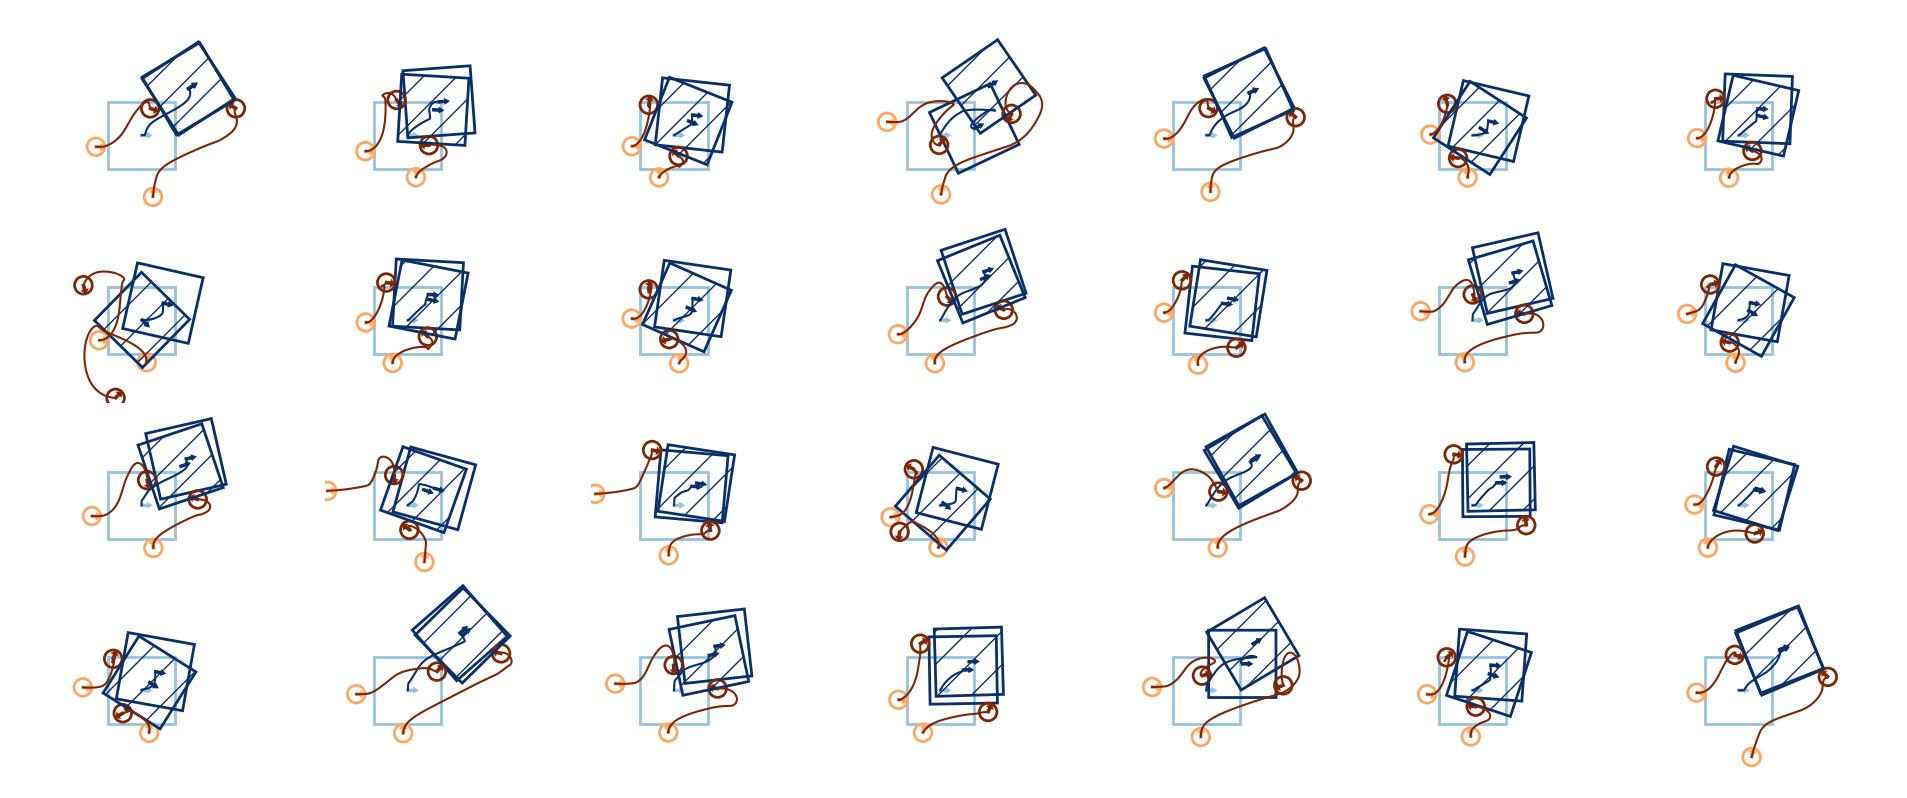
\includegraphics[width=\linewidth]{images/ch5/mam_more.png}
    \caption{Additional examples of optimized multi-agent manipulation behavior in simulation, showing that the optimized strategy reaches the goal in most cases. Each example shows the results of executing the optimized pushing strategy for \SI{4}{s} with a randomly selected set of friction coefficients, random target pose, and random initial robot poses. Light/dark colors indicate initial/final positions, and the striped box indicates the target pose.}
    \label{app:ch5:fig:mam_more}
\end{figure}

To assess the robustness and efficiency of this design optimization method, we must answer a number of questions. For instance, how does automatic differentiation compare with other methods for estimating the gradient (e.g. finite differences)? What benefit does variance regularization in problem~\eqref{ch5:eq:design_optimization_nlp} bring? We answer these questions here using an ablation study where we attempt to isolate the impact of each of these features.

First, why use automatic differentiation? On the one hand, AD allows us to estimate the gradient with only a single evaluation of the objective function, while other methods (such as finite differences, or FD) require multiple evaluations. On the other hand, AD necessarily incurs some overhead at runtime, making each AD function call more expensive than those used in an FD scheme. Additionally, some arguments~\cite{suh2021_bundled_gradients} suggest that exact gradients may be less useful than finite-difference or stochastic approximations when the objective is stiff or discontinuous. We compare AD with a 3-point finite-difference method by re-solving problem~\eqref{ch5:eq:design_optimization_nlp} for both case studies, keeping all parameters constant ($N=512$, $\lambda=0.1$, same random seed) and substituting the gradients obtained using AD for those computed using finite differences. Fig.~\ref{ch5:fig:ablation} shows the results of this comparison. In the sensor placement example, AD achieves a lower expected cost and cost variance, and it runs in 32\% less time. In the collaborative manipulation example, both methods achieve similar expected cost and variance, but the AD version runs nearly 19x faster. These results lead us to conclude that AD enables more effective optimization than finite differences and is an appropriate choice for our framework.

The next question is whether variance regularization brings any benefit to the design optimization problem. To answer this question, we compare the results of re-solving both case studies with variance weight $\lambda = 0.1$ and $\lambda = 0$. These results are shown in Fig.~\ref{ch5:fig:ablation}; surprisingly, in the sensor placement example we see that the variance-regularized problem results in a lower expected cost, contrary to the intuition that regularization requires a trade off with increased expected cost. We expect that this lower expected cost may be a result of the regularization term smoothing the objective with respect to the exogenous parameters. However, these benefits are less pronounced than the benefits from automatic differentiation, and we see more benefit in the sensor-placement example reported in~\cite{dawsonCertifiableRobotDesign2022a} than in the multi-agent manipulation problem.

\begin{figure}[t]
    \centering
    \begin{subfigure}[t]{0.25\linewidth}
        \centering
        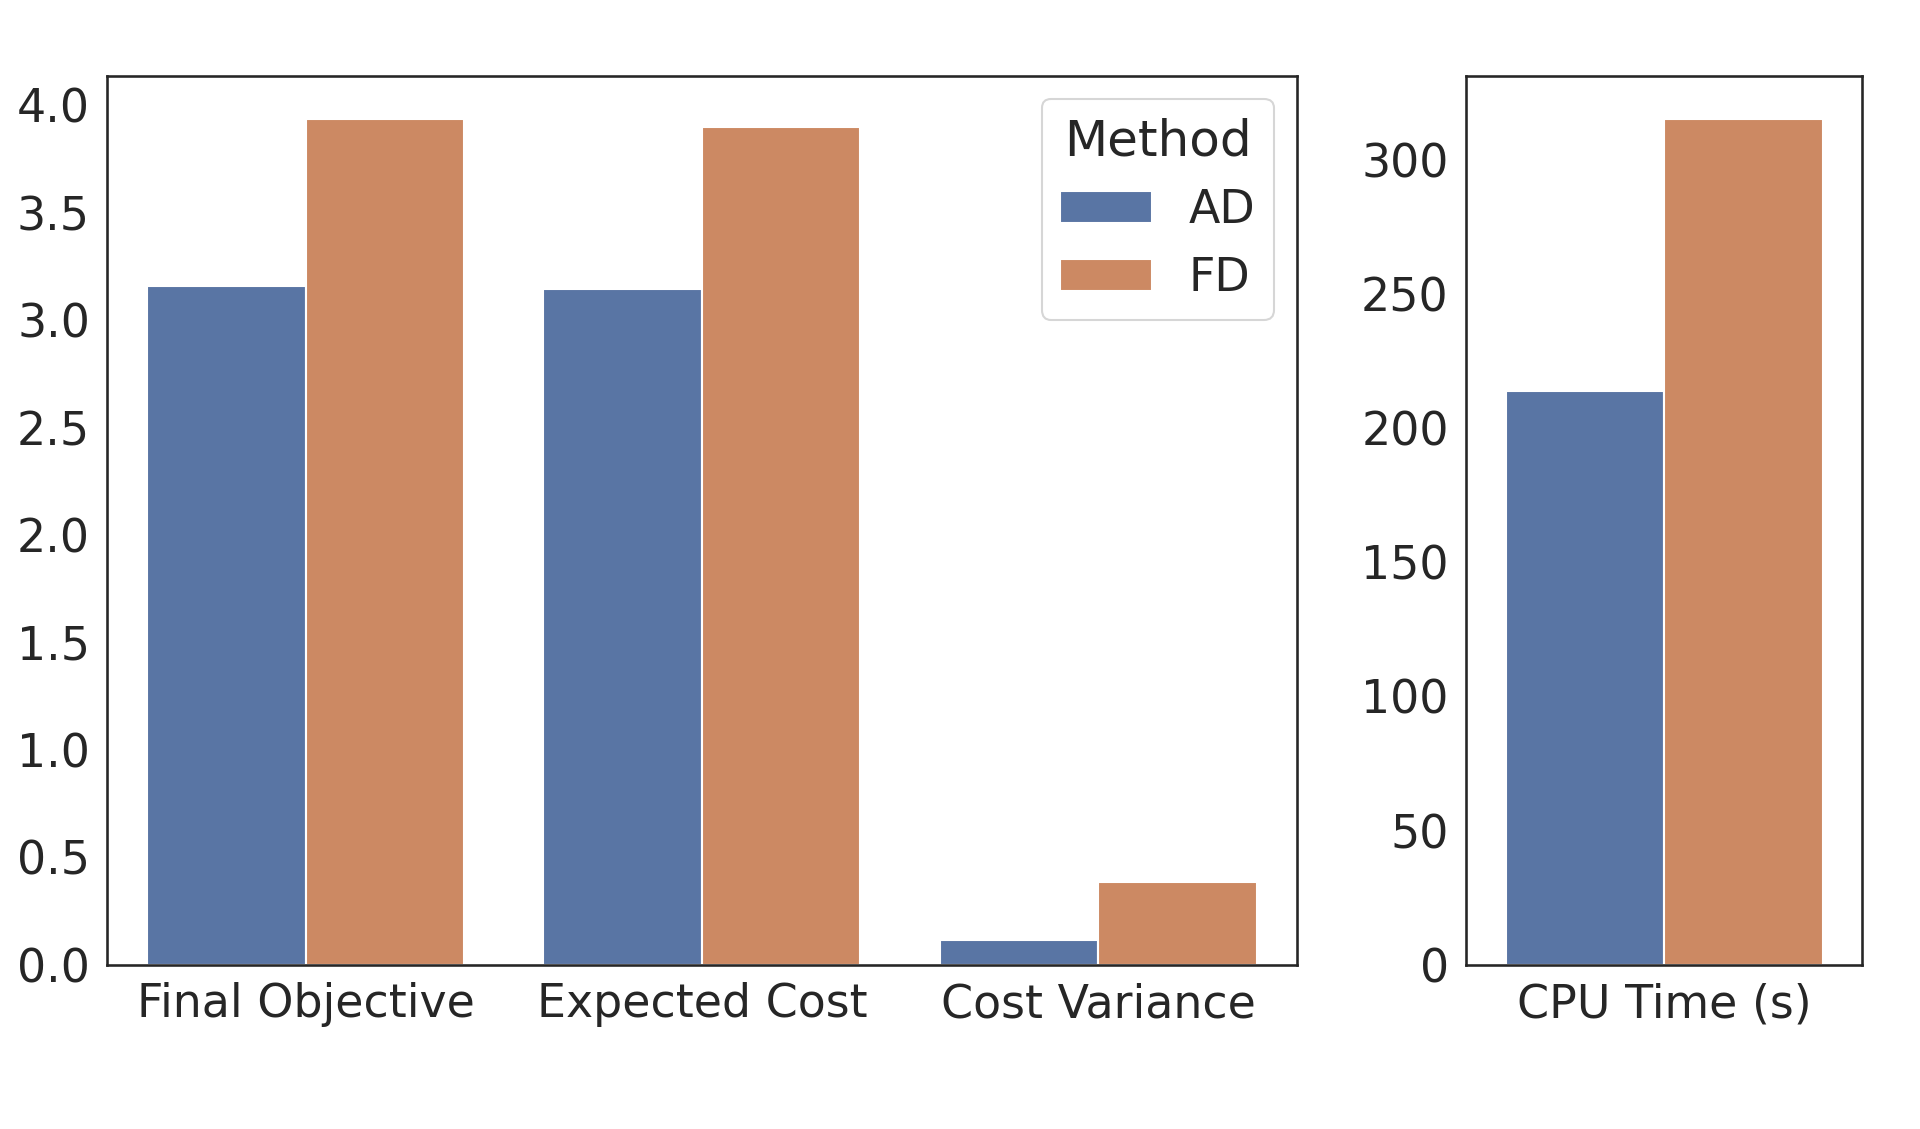
\includegraphics[width=\linewidth]{images/ch5/agv_ad_fd_ablation.png}
        \caption{AD vs. FD; sensor placement}
    \end{subfigure}%
    % \ \\
    % \ \\
    \begin{subfigure}[t]{0.25\linewidth}
        \centering
        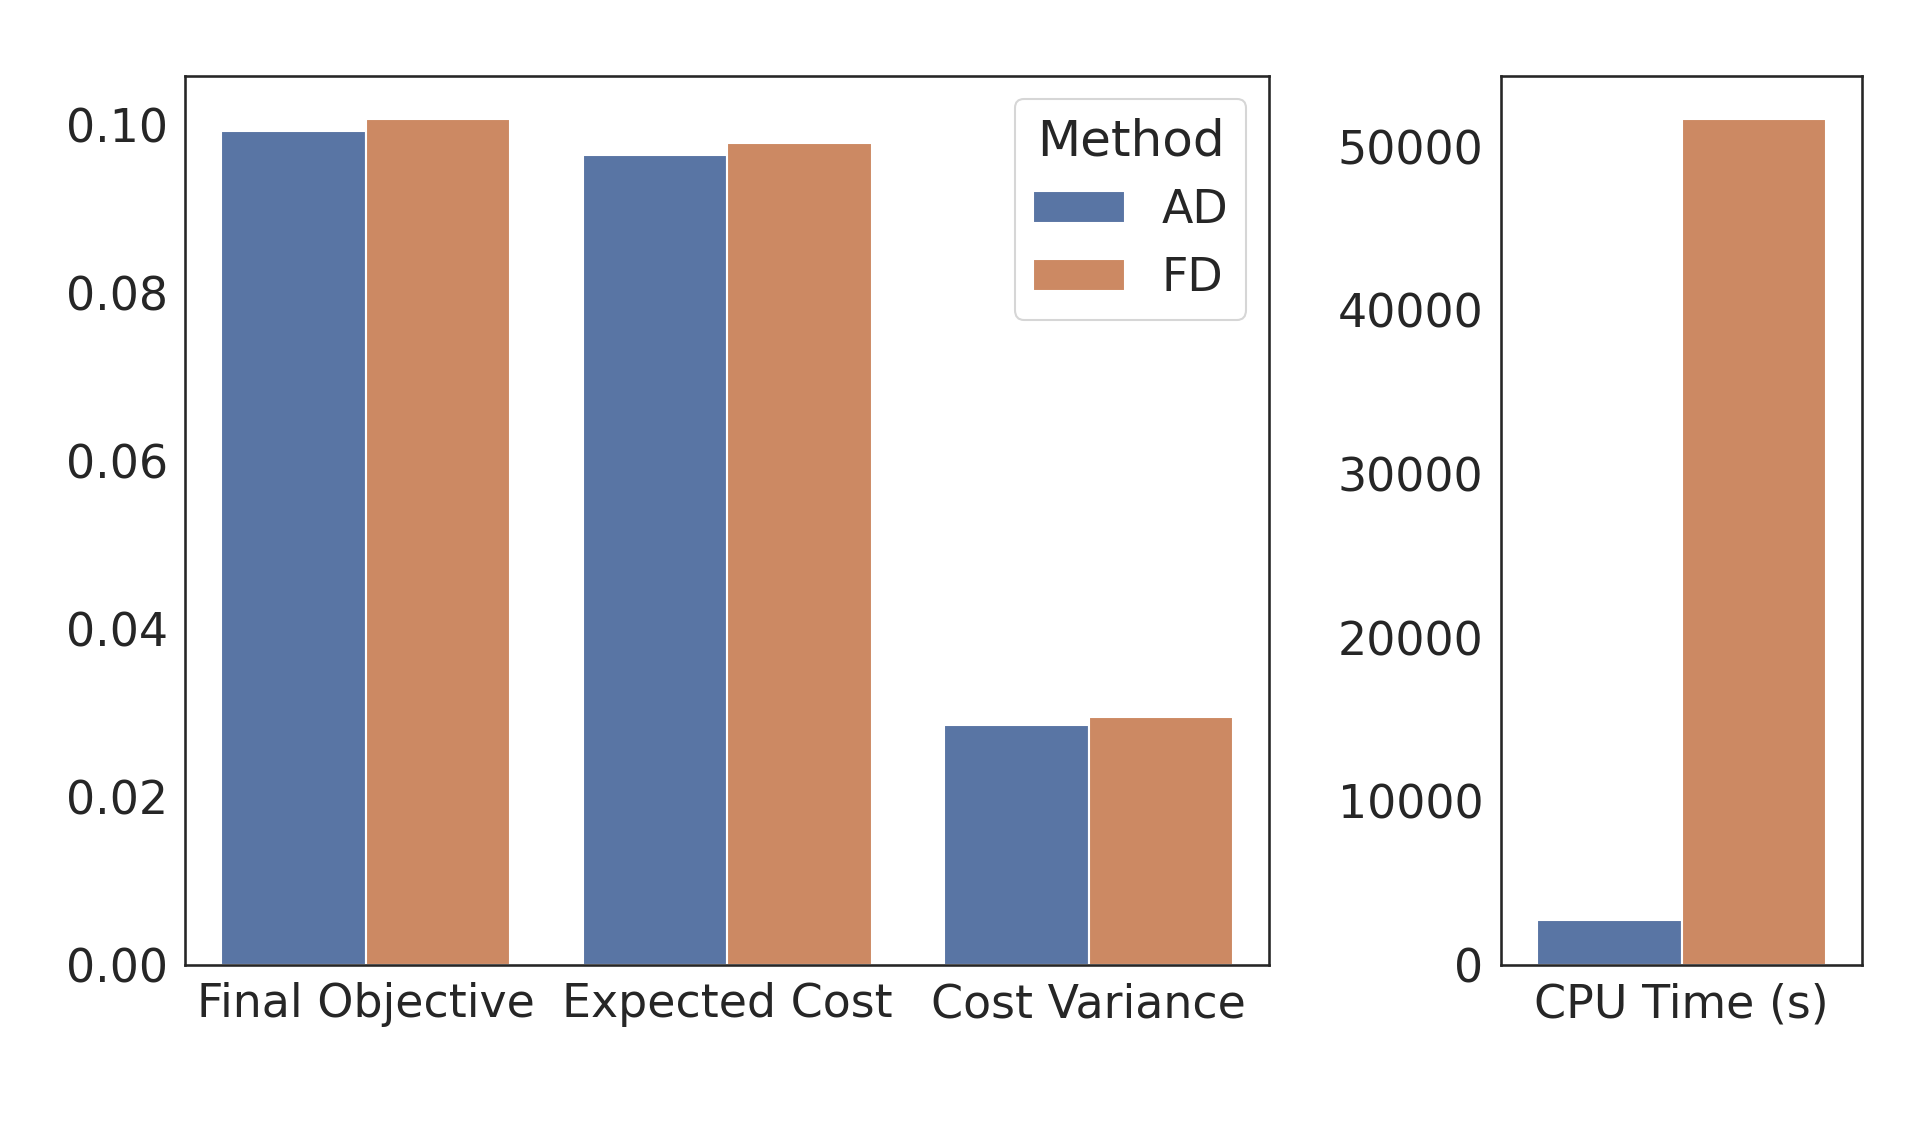
\includegraphics[width=\linewidth]{images/ch5/mam_ablation_ad_fd.png}
        \caption{AD vs. FD; manipulation}
    \end{subfigure}%
    \begin{subfigure}[t]{0.25\linewidth}
        \centering
        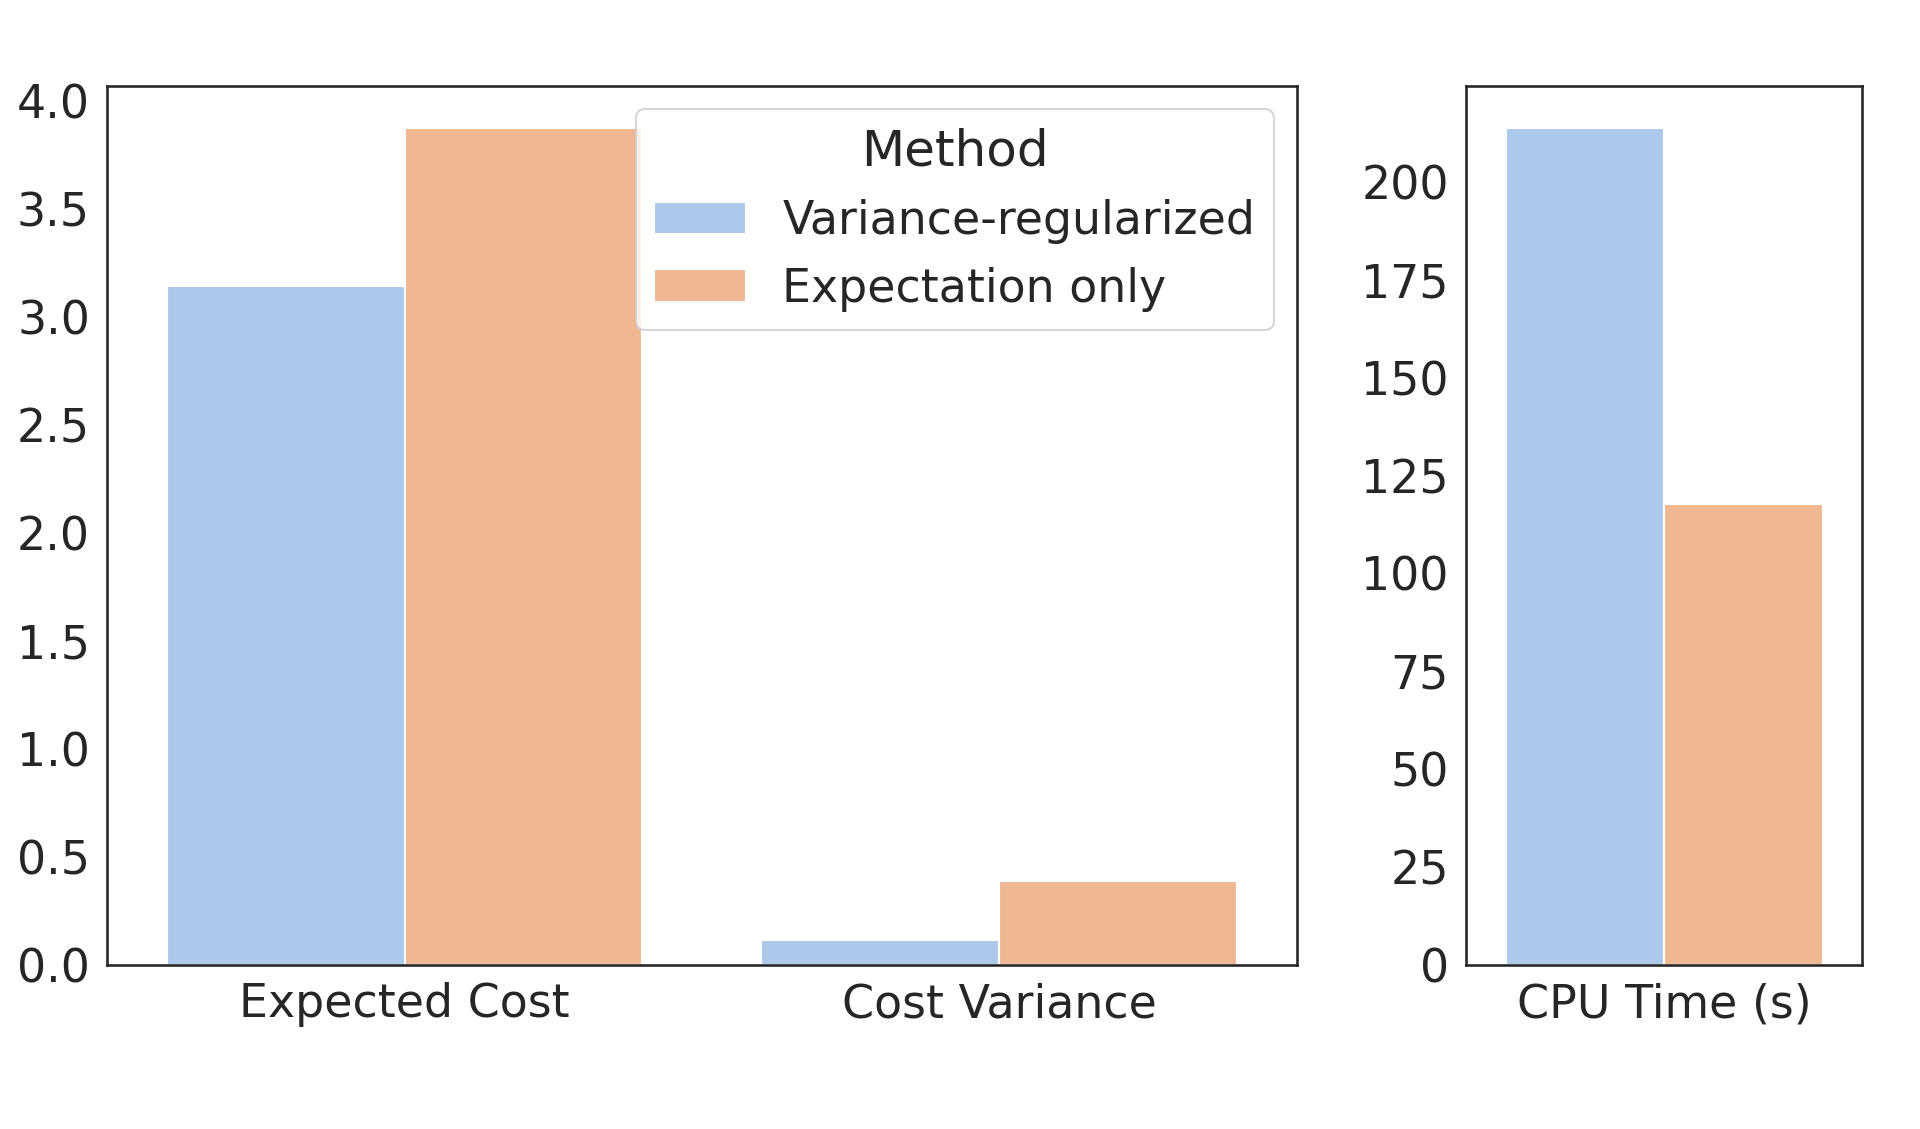
\includegraphics[width=\linewidth]{images/ch5/agv_vr_ablation.png}
        \caption{VR; sensor placement}
    \end{subfigure}%
    % \ \\
    % \ \\
    \begin{subfigure}[t]{0.25\linewidth}
        \centering
        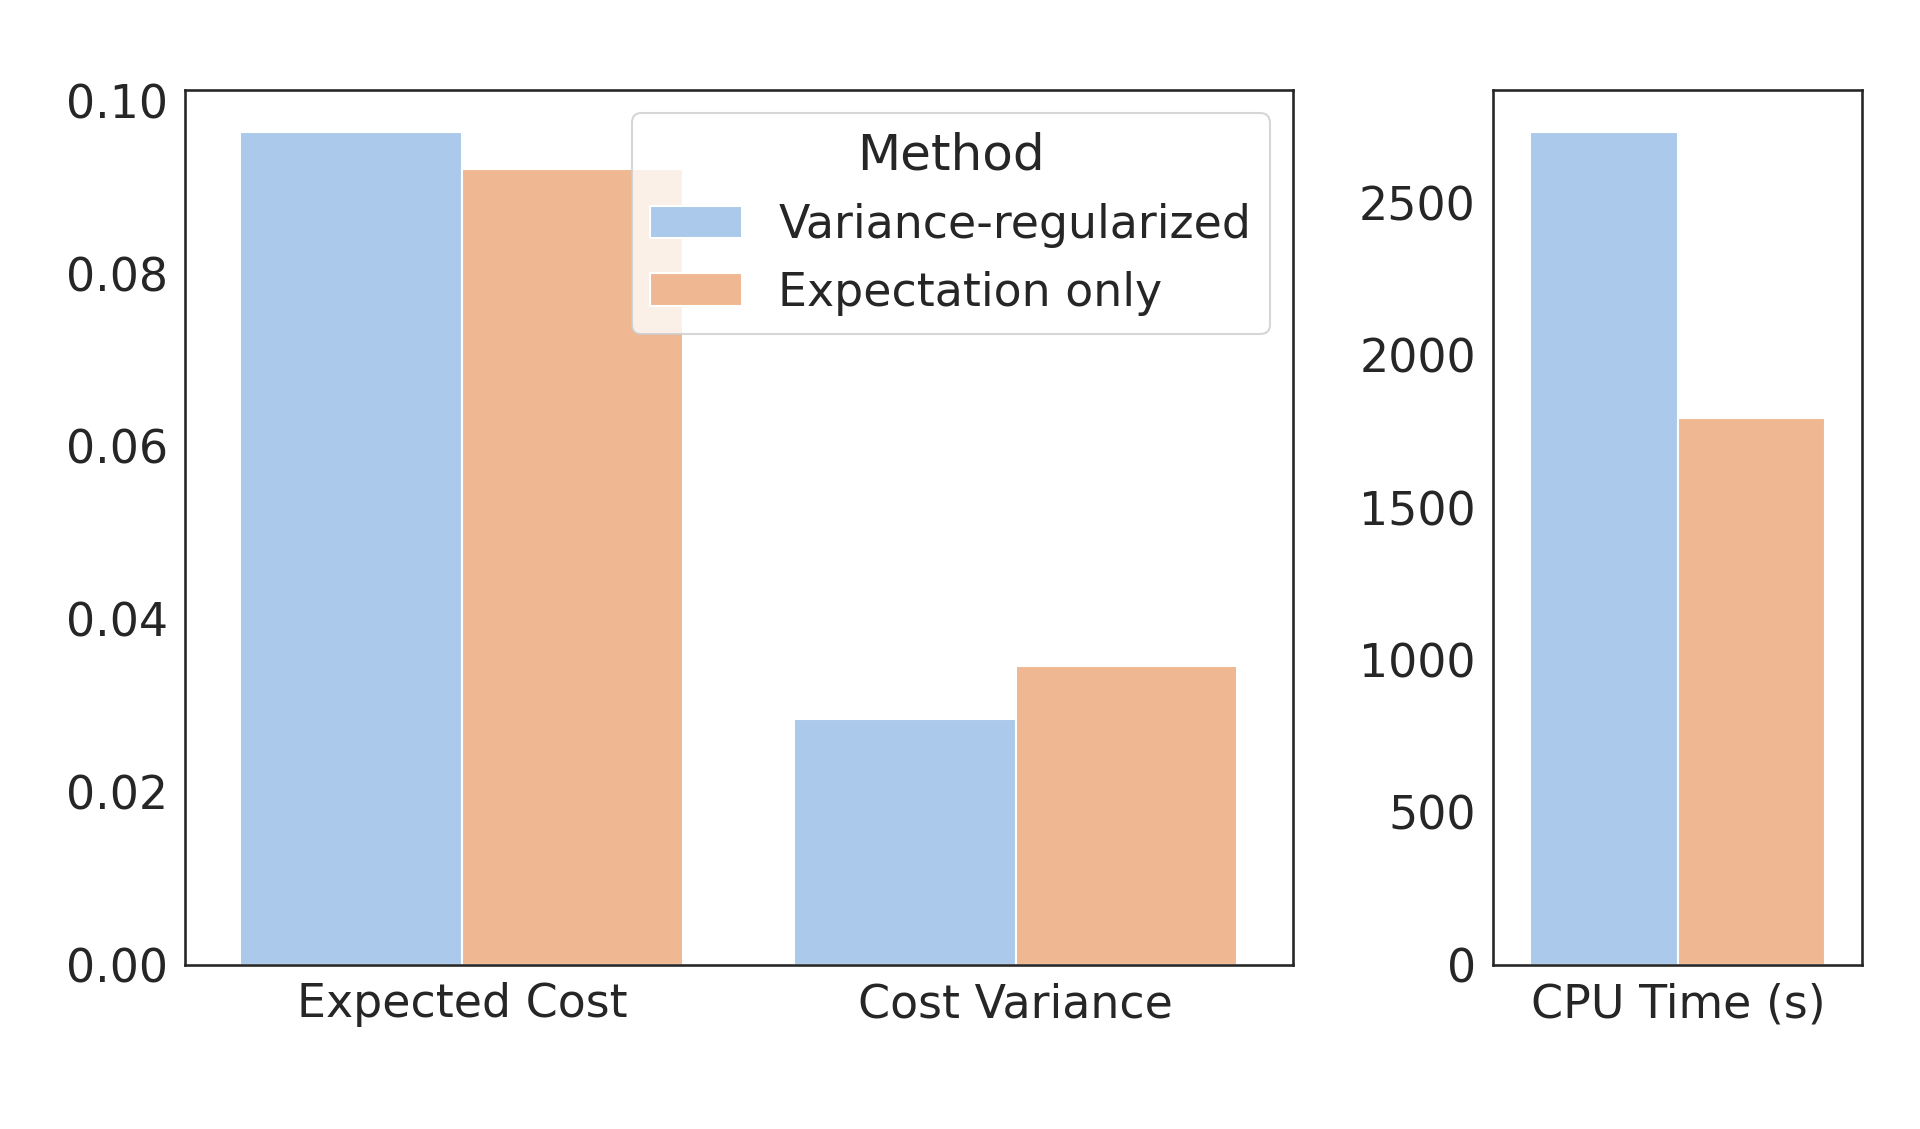
\includegraphics[width=\linewidth]{images/ch5/mam_ablation_vr.png}
        \caption{VR; manipulation}
    \end{subfigure}
    \caption{(a)-(b) Improvement of automatic differentiation (AD) over finite differences (FD) in both case studies. (c)-(d) Effect of variance regularization (VR) in both case studies.}
    \label{app:ch5:fig:ablation}
\end{figure}

\subsection{Details on satellite trajectory planning case study}

We can express this problem using dynaimcs in the Clohessy-Wiltshire-Hill coordinate frame~\cite{jewisonSpacecraftBenchmarkProblem2016}, which assumes that the target's orbit is circular and constructs a coordinate frame with the origin at the target, the $x$-axis pointing away from the Earth, the $y$-axis pointing along the target's orbit, and the $z$-axis pointing out of the orbital plane. In this frame, the chaser's dynamics are approximately linear, with positions $p_x$, $p_y$, $p_z$ and velocities $v_x$, $v_y$, $v_z$ varying according to controlled thrust in each direction $u_x$, $u_y$, $u_z$:
\begin{align*}
    \mat{\dot{p}_x              \\ \dot{p}_y \\ \dot{p}_z \\ \dot{v}_x \\ \dot{v}_y \\ \dot{v}_z} = \mat{
    v_x                         \\
    v_y                         \\
    v_z                         \\
    3n^2 p_x + 2n v_y + u_x / m \\
    -2n v_x + u_y / m           \\
        -n^2 p_z + u_z / m
    }
\end{align*}
%
$n = \sqrt{\mu / a^3}$ is the mean-motion of the target, determined by the Earth's gravitational constant $\mu = \SI{3.986e14}{m^3/s^2}$ and the target's altitude $a$ (i.e. the length of the semi-major orbital axis, \SI{353}{km} in low Earth orbit). $m = \SI{500}{kg}$ is the mass of the chaser satellite~\cite{jewisonSpacecraftBenchmarkProblem2016}.

%---------------------------------------------------------------------------%
%								 End Document								%
%---------------------------------------------------------------------------%
\end{document}
